% This is part of Un soupçon de mathématique sans être agressif pour autant
% Copyright (c) 2012-2014
%   Laurent Claessens
% See the file fdl-1.3.txt for copying conditions.

\documentclass[a4paper,12pt]{book}
% This is part of Un soupçon de mathématique sans être agressif pour autant
% Copyright (c) 2012-2014
%   Laurent Claessens
% See the file fdl-1.3.txt for copying conditions.


\usepackage{etex}
\usepackage{ifthen}
%\usepackage{pdfsync}       % This package is obsolete : compile with pdflatex -synctex=1 instead.

\usepackage{latexsym}
\usepackage{amsfonts}
\usepackage{amsmath}
\usepackage{amsthm}
\usepackage{amssymb}
\usepackage{bbm}
\usepackage{mathrsfs}           
\usepackage{mathabx}           % Pour \divides

\usepackage{framed} % pour oframed
\usepackage{wrapfig}

\usepackage{calc}   % Les dépendances de phystricks si on n'utilise que le pdf.
%\usepackage{pstricks,pst-eucl,pstricks-add,calc,pst-math}   % Les dépendances de phystricks. Peut être qu'il faut ajouter catchfile


% Les dépendances de phystricks en mode Tikz
\usepackage{tikz}
\usepackage{calc}
\usetikzlibrary{calc}
\usetikzlibrary{patterns}

\usetikzlibrary{external}
\tikzexternalize
%\newcommand{\tikzsetnextfilename}[1]{}
\newcounter{defHatch}
\newcounter{defPattern}
\setcounter{defHatch}{0}
\setcounter{defPattern}{0}


\usepackage{graphicx}                   % Pour l'inclusion d'image en pfd.

%\newcommand{\EpsOrPdfincludegraphics}[2][]{%
%        \ifpdf
%            \includegraphics[#1]{#2.png}
%        \else
%            \includegraphics[#1]{#2.eps}
%        \fi
%        }

\usepackage{subfigure}

\usepackage{fancyvrb}
\usepackage{stmaryrd}       % Pour le \obslash
\usepackage{xstring}        % Utilisé pour les références vers wikipédia
\usepackage{cases}
\usepackage{lscape}         % pour l'environnement landscape, utilisé dans la correction corr0076.tex
\usepackage{multicol}
\setlength{\columnseprule}{0.5pt}
\usepackage{import}         % Pour le hack qui sert à inclure GeomAnal

% TODO : n'en utiliser qu'un
\usepackage[normalem]{ulem}     % Pour le barré, commande \sout
\usepackage{soul}       % Pour le barré, commande \st

\usepackage[all]{xy}

\let\second\undefined      % le paquet amthabx définit \second
\let\degree\undefined       % le paquet amthabx définit \degree
%\usepackage[cdot,thinqspace,amssymb]{SIunits} 
\usepackage[parse-numbers=false,binary-units=true,detect-all=true,per-mode=symbol]{siunitx} 
\newcommand{\unit}[2]{\SI{#1}{#2}}
 % L'option amssymb sert à éviter un conflit avec la commande \square de amssymb. Note qu'elle n'est plus accessible. Si tu en as besoin, faudra RTFM
%ftp://ftp.belnet.be/packages/ctan/macros/latex/contrib/SIunits/SIunits.pdf

\usepackage[nottoc]{tocbibind}
\usepackage[numbers]{natbib}

%%%%%%%%%%%%%%%%%%%%%%%%%%
%
%   Trucs mathématiques
%
%%%%%%%%%%%%%%%%%%%%%%%%

% ENSEMBLES DE NOMBRES
\newcommand{\eA}{\mathbbm{A}}
\newcommand{\eC}{\mathbbm{C}}
\newcommand{\eD}{\mathbbm{D}}
\newcommand{\eE}{\mathbbm{E}}
\newcommand{\eF}{\mathbbm{F}}
\newcommand{\eG}{\mathbbm{G}}
\newcommand{\eH}{\mathbbm{H}}
\newcommand{\eK}{\mathbbm{K}}
\newcommand{\eL}{\mathbbm{L}}
\newcommand{\eM}{\mathbbm{M}}
\newcommand{\eN}{\mathbbm{N}}
\newcommand{\eP}{\mathbbm{P}}
\newcommand{\eQ}{\mathbbm{Q}}
\newcommand{\eR}{\mathbbm{R}}
\newcommand{\eZ}{\mathbbm{Z}}

% ENSEMBLES de fonctions
\newcommand{\aL}{\mathcal{L}}       % Les applications linéaires
\newcommand{\aC}{\mathcal{C}}       % Les fonctions C^1, C^2 etc



\newcommand{\mF}{\mathcal{F}}
\newcommand{\mC}{\mathcal{C}}
\newcommand{\mG}{\mathcal{G}}
\newcommand{\mI}{\mathcal{I}}
\newcommand{\mL}{\mathcal{L}}
\newcommand{\mS}{\mathcal{S}}   % Utilisé pour l'espace des fonctions Schwartz
\newcommand{\mZ}{\mathcal{Z}}


\newcommand{\mtu}{\mathbbm{1}}              % La matrice unité

\DeclareMathOperator{\val}{val}     % valuation d'un polynôme
%\DeclareMathOperator{\opp}{opp}    % Les nombres négatifs


%\newcommand{\efrac}[2]{\frac{ \displaystyle #1 }{\displaystyle #2 }}
%%%%%%%%%%%%%%%%%%%%%%%%%%
%
%   Numérotations en tout genre
%
%%%%%%%%%%%%%%%%%%%%%%%%

\setcounter{tocdepth}{2}        % Profondeur de la table des matières
\setcounter{secnumdepth}{2}     % Profondeur dans le texte

\renewcommand{\thesubsection}{\thesection.\alph{subsection}}

%%%%%%%%%%%%%%%%%%%%%%%%%%
%
%   Les lignes magiques pour le texte en français.
%
%%%%%%%%%%%%%%%%%%%%%%%%

\usepackage[utf8]{inputenc}
\usepackage[T1]{fontenc}

\usepackage{listingsutf8}
%\lstset{language=python,basicstyle=\footnotesize,tabsize=3,numbers=left,numberstyle=\tiny,frame=single,commentstyle=\ttfamily\color[rgb]{0,0,0.5},stringstyle=\color[rgb]{0,0.5,0},title=\lstname,inputencoding=utf8/latin1}
\lstset{language=python,basicstyle=\footnotesize,tabsize=3,frame=single,commentstyle=\ttfamily\color[rgb]{0,0,0.5},stringstyle=\color[rgb]{0,0.5,0},title=\lstname,inputencoding=utf8/latin1}

\usepackage[fr]{exocorr}
\usepackage{textcomp}
\usepackage{lmodern}
\usepackage[a4paper,margin=2cm]{geometry} 
\usepackage[english,frenchb]{babel}


\usepackage{hyperref}                           %Doit être appelé en dernier.
\hypersetup{
colorlinks=true,
linkcolor=blue,
urlcolor=magenta,     % couleur des url
filecolor=magenta   % couleur des textes qui sont des liens
}

% Il me semble que cette commande doit être définie après l'appel à Babel.
\newcommand{\Ieme}{\up{\lowercase{ième}}\xspace}

%%%%%%%%%%%%%%%%%%%%%%%%%%
%
%   Les théorèmes et choses attenantes
%
%%%%%%%%%%%%%%%%%%%%%%%%


\newcounter{numtho}
\newcounter{numprob}

\makeatletter
\@addtoreset{numtho}{chapter}
%\@addtoreset{CountExercice}{chapter}
\@addtoreset{chapter}{part}
\makeatother

\newlength{\EnvSpace}
\setlength{\EnvSpace}{9pt}      % C'est la distance que je veux mettre avant et après les théorèmes, remarques, etc.

\newtheoremstyle{MyTheorems}%
        {\EnvSpace}{\EnvSpace}%
        {\itshape}%
        {}%
        {\bfseries}{.}%
        {\newline}%
        {}%
\newtheoremstyle{MyExamples}%
        {\EnvSpace}{\EnvSpace}%
        {}%
        {}%
        {\bfseries}{.}%
        {\newline}%
        {}%
\newtheoremstyle{MyRemarks}%
        {\EnvSpace}{\EnvSpace}%
        {}%
        {}%
        {\bfseries}{.}%
        {\newline}%
        {}%

%\theoremstyle{MyExamples}   %\newtheorem{exemple}[numtho]{Exemple}      % Pour unification, ne plus utiliser
%                            \newtheorem{example}[numtho]{Exemple}
\newcounter{CounterExample}
\renewcommand{\theCounterExample}{\thechapter.\arabic{CounterExample}}

% J'ai décidé de ne plus numéroter les choses encadrées. 8 avril 2014
\newenvironment{example}{\vspace{\EnvSpace}\refstepcounter{numtho}\noindent{\bf Exemple}\\\nopagebreak}{\phantom{a}\hfill $\triangle$\vspace{\EnvSpace}}
\newenvironment{Aretenir}{\refstepcounter{numtho}\begin{oframed}\noindent{\bf À retenir}\newline}{\end{oframed}\vspace{\EnvSpace}}
\newenvironment{Aprojeter}{\clearpage\phantom{a}\vfill}{\vfill\newpage}
\newenvironment{definition}[1][]{\refstepcounter{numtho}\begin{oframed}\noindent{\bf Définition}#1\newline}{\end{oframed}\vspace{\EnvSpace}}
\newenvironment{propriete}{\refstepcounter{numtho}\begin{oframed}\noindent{\bf Propriété}\newline}{\end{oframed}\vspace{\EnvSpace}}

\newenvironment{Enmini}{\begin{oframed}\noindent{\bf Mini résumé}\newline}{\end{oframed}\vspace{\EnvSpace}}
% Ce bout de code provient de BrunoJ
% https://brunoj.wordpress.com/2009/10/08/latex-the-framed-minipage/
\newsavebox{\fmbox}
 \newenvironment{fmpage}[1]
 {\begin{lrbox}{\fmbox}\begin{minipage}{#1}}
     {\end{minipage}\end{lrbox}
     \fbox{\usebox{\fmbox}}
 }

\theoremstyle{MyRemarks}    \newtheorem{remark}[numtho]{Remarque}

                \newtheorem{amusement}[numtho]{Amusement}
                \newtheorem{erreur}[numtho]{Error}
                \newtheorem{probleme}[numprob]{\fbox{\bf Problèmes et choses à faire}}


\theoremstyle{MyTheorems}
\newtheorem{lemma}[numtho]{Lemme}
\newtheorem{corollary}[numtho]{Corollaire}
\newtheorem{theorem}[numtho]{Théorème}      
\newtheorem{proposition}[numtho]{Proposition}      


\renewcommand{\thenumtho}{\thechapter.\arabic{numtho}}
% La numérotation des équations change dans les corrigés
\renewcommand{\theequation}{\thechapter.\arabic{equation}}
\renewcommand{\theCountExercice}{\arabic{CountExercice}}       % Ce compteur est défini dans SystemeCorr.sty
\newcommand{\defe}[2]{\textbf{#1}\index{#2}}

\renewcommand{\theenumi}{(\alph{enumi})}
\renewcommand{\theenumii}{(\alph{enumi}\arabic{enumii})}

\renewcommand{\labelenumi}{\theenumi}
\renewcommand{\labelenumii}{\theenumii}

\newcommand{\justification}{ {\small \begin{center}    Attention : vous devez laisser sur votre feuille les traces de vos recherches et les étapes intermédiaires de vos calculs !    \end{center}}}
    

    % L'une des deux est avec le nom et l'autre sans.
    \newenvironment{feuilleDS}[1]{\noindent Nom, Prénom : \begin{center}\large #1\\\justification\end{center}\setcounter{CountExercice}{0}  }{\clearpage}
    %\newenvironment{feuilleDS}[1]{\begin{center}\large #1\\\justification\end{center}\setcounter{CountExercice}{0}  }{\clearpage}


    \newenvironment{feuilleExo}[1]{\newpage\begin{center}\large #1\end{center}\setcounter{CountExercice}{0}  }{\clearpage}
    %\newenvironment{feuilleExo}[1]{\begin{center}\large #1\end{center}\setcounter{CountExercice}{0}  }{}

        
        \newcounter{numactivmentale}
        \setcounter{numactivmentale}{0}
        \newcounter{numExoMental}
        \setcounter{numExoMental}{0}
        \newenvironment{MentalActivity}{\setcounter{numExoMental}{0}\newpage\refstepcounter{numactivmentale}\section{Activité mentale \arabic{numactivmentale}}}{\newpage\hphantom{jj}\vfill\large C'est tout pour aujourd'hui\vfill\newpage}
        \newenvironment{mental}{\refstepcounter{numExoMental}\newpage\begin{center}\fbox{\huge Activité mentale \arabic{numactivmentale}}\\\huge Question \arabic{numExoMental}\end{center}\huge\vfill}{\vfill}


\newcommand{\enteteInterro}[3]{
    \begin{center}
        #1\\
        Intérogation #2, sujet #3
    \end{center}
    Nom, prénom, classe : \ldots\\
    \setcounter{CountExercice}{0}
}


%%%%%%%%%%%%%%%%%%%%%%%%%%
%
%   Les macros qui font des choses
%
%%%%%%%%%%%%%%%%%%%%%%%%

\newcommand{\mA}{\mathcal{A}}
\newcommand{\mO}{\mathcal{O}}
\newcommand{\mR}{\mathcal{R}}
\newcommand{\mT}{\mathcal{T}}
\newcommand{\mU}{\mathcal{U}}

\newcommand{\scal}[2]{ \langle #1,#2\rangle }

\newcommand{\tq}{\text{ tel que }}
\newcommand{\tqs}{\text{ tels que }}
\newcommand{\quext}[1]{ \footnote{\textsf{#1}}  }
\newcommand{\info}[1]{\texttt{#1}}
\newcommand{\vect}[1]{\overrightarrow{#1}}    % Cette macro est codée en dur dans phystricksDefVecteurAXDDGP et dans d'autres

\newcommand{\VarAbs}{\text{Var}_{\text{abs}}}
\newcommand{\VarRel}{\text{Var}_{\text{rel}}}

\newcommand{\normal}{\lhd}
\newcommand{\swS}{\mathscr{S}}          % L'ensemble des fonctions Schwartz

%\newcommand{\defD}{\mathscr{D}}     % Ensemble de définition d'une fonction
\newcommand{\defD}{D}                % Le D avec des croles était impossible à comprendre pour les élèves.

\newcommand{\Borelien}{\mathcal{B}\text{or}}       % Les boréliens
\newcommand{\tribA}{\mathcal{A}}            % Une tribu A
\newcommand{\tribB}{\mathcal{B}}            
\newcommand{\tribF}{\mathcal{F}}            % Une tribu F

\newcommand{\affE}{\mathcal{E}}            % Un espace affine E
\newcommand{\affF}{\mathcal{F}}            
\newcommand{\affG}{\mathcal{G}}            

\newcommand{\statS}{\mathcal{S}}            % Un modèle statistique
\newcommand{\partP}{\mathcal{P}}            % L'ensemble des parties d'un ensemble

\newcommand{\polyP}{\mathcal{P}}            % L'ensemble des polynômes

\newcommand{\dB}{\mathscr{B}}       % la distribution de Bernoulli
\newcommand{\dE}{\mathscr{E}}       % la distribution exponentielle
\newcommand{\dG}{\mathscr{G}}       % la distribution géométrique.
\newcommand{\dM}{\mathscr{M}}       % la distribution multinomiale
\newcommand{\dN}{\mathscr{N}}       % la distribution normale.
\newcommand{\dP}{\mathscr{P}}       % la distribution de Poisson.
\newcommand{\dT}{\mathscr{T}}       % la distribution de Student
\newcommand{\dU}{\mathscr{U}}       % la distribution uniforme

\newcommand{\hL}{\mathscr{L}}       
\newcommand{\cL}{\hL}           % Pour la partie Chafai

\newcommand{\modE}{\mathcal{E}}         % Le E des modules
\newcommand{\modF}{\mathcal{F}}         % Le F des modules
\newcommand{\hH}{\mathscr{H}}           % Le H des espaces de Hilbert

%%%%%%%%%%%%%%%%%%%%%%%%%%
%
%   Bibliographie, index et liste des notations
%
%%%%%%%%%%%%%%%%%%%%%%%%

\usepackage{makeidx}
\usepackage[nottoc]{tocbibind}      % Le paquetage qui fait en sorte que la biblio soit inclue correctement dans la table des matières.
\usepackage[refpage]{nomencl}
\renewcommand{\nomname}{Liste des notations}
%
%   Comment introduire des éléments dans l'index des notations.
%
% La liste des tags à mettre pour bien classer mes notations est :
% T     pour la topologie et théorie des ensembles
%
% La syntaxe est facile, par exemple 
%       $\SL(2,\eR)$\nomenclature[G]{$\SL(2,\eR)$}{Le groupe de matrices deux par deux de déterminant 1.}
%\renewcommand{\nomgroup}[1]{%
%    \ifthenelse{\equal{#1}{A}}{\item[\textbf{Algèbre}]}{}%
%    \ifthenelse{\equal{#1}{G}}{\item[\textbf{Géométrie}]}{}%
%    \ifthenelse{\equal{#1}{R}}{\item[\textbf{Théorie des groupes}]}{}%
%    \ifthenelse{\equal{#1}{P}}{\item[\textbf{Probabilités et statistique}]}{}%
%    \ifthenelse{\equal{#1}{Y}}{\item[\textbf{Analyse}]}{}%
%    \ifthenelse{\equal{#1}{M}}{\item[\textbf{Chaînes de Markov}]}{}%
%}

%%%%%%%%%%%%%%%%%%%%%%%%%%
%
%   DeclareMathOperator
%
%%%%%%%%%%%%%%%%%%%%%%%%

\DeclareMathOperator{\signe}{sgn}
\DeclareMathOperator{\Vol}{Vol}
\DeclareMathOperator{\Int}{Int}     % Intérieur d'un ensemble.
\DeclareMathOperator{\Ind}{Ind}     % l'indice d'un chemin en analyse complexe
\DeclareMathOperator{\Diam}{Diam}   
\DeclareMathOperator{\id}{Id}   
\DeclareMathOperator{\Graph}{Graph} 
\DeclareMathOperator{\pr}{\texttt{proj}}
\DeclareMathOperator{\dom}{dom}

\DeclareMathOperator{\Graphe}{Gr}
\DeclareMathOperator{\Spec}{Spec}   % spectre d'un opérateur
\DeclareMathOperator{\arctg}{arctg}
\DeclareMathOperator{\cotg}{cotg}
\DeclareMathOperator{\cosec}{cosec}
\DeclareMathOperator{\arcsinh}{arcsinh}

\DeclareMathOperator{\GL}{GL}   % le groupe linéaire
\DeclareMathOperator{\PGL}{PGL}   % le groupe projectif
\DeclareMathOperator{\SO}{SO}           
\DeclareMathOperator{\SL}{SL}           
\DeclareMathOperator{\PSL}{PSL}   % Le groupe modulaire SL(2,Z)/Z2
\DeclareMathOperator{\gO}{O}           
\DeclareMathOperator{\SU}{SU}           
\DeclareMathOperator{\gU}{U}           

\DeclareMathOperator{\Reel}{Re}        % La partie réelle d'un nombre complexe

\DeclareMathOperator{\Image}{Image}        % ... avec \Image qui donne l'image d'une fonction ou d'un opérateur.
\DeclareMathOperator{\rang}{rg}   
\DeclareMathOperator{\Kernel}{Ker}
\DeclareMathOperator{\Domaine}{Dom}
\DeclareMathOperator{\Span}{Span}
\DeclareMathOperator{\Hom}{Hom}
\DeclareMathOperator{\End}{End}     % L'ensemble des endomorphismes
\DeclareMathOperator{\tr}{Tr}       % la trace
\DeclareMathOperator{\Majorant}{Maj}
\DeclareMathOperator{\codim}{codim} % pour la codimension.
\DeclareMathOperator{\diam}{diam} % le diamètre d'un ensemble.

\DeclareMathOperator{\Var}{Var}     % Variance d'une variable aléatoire.
\DeclareMathOperator{\Fun}{\texttt{Fun}}     % Ensemble des applications d'un ensemble vers l'autre.
\DeclareMathOperator{\Cov}{Cov}     % la covariance.
\DeclareMathOperator{\gr}{gr}     % le groupe engendré
\DeclareMathOperator{\pgcd}{pgcd}     
\DeclareMathOperator{\ppcm}{ppcm}     
\DeclareMathOperator{\Frob}{Frob}     
\DeclareMathOperator{\Card}{Card}       % Le cardinal d'un ensemble.
\DeclareMathOperator{\Stab}{Stab}       % Le stabilisateur d'un point sous l'action d'un groupe.

\DeclareMathOperator{\Frac}{Frac}       % le corps des fractions d'un anneau
\DeclareMathOperator{\Aff}{Aff}         %  l'espace affine engendré

\newenvironment{subproof}{\begin{description}}{\end{description}}

\newcommand{\telque}{\vert\,}
\newcommand{\donc}{\Rightarrow}

\usepackage{mathtools}
\mathtoolsset{showonlyrefs}

%\renewcommand{\thechapter}{\Roman{chapter}}    


%TODO : il faudra fusioner avec echa un jour; oui monsieur : tout echa même la physique.

% Il faut lire README.txt

\begin{document}


\corrPosition{2}
%\corrDraft{1}

% This is part of Un soupçon de mathématique sans être agressif pour autant
% Copyright (c) 2012
%   Laurent Claessens
% See the file fdl-1.3.txt for copying conditions.

\thispagestyle{empty}
\begin{center}
  \begin{minipage}{15cm}
    \hrule\par
    \vspace{2mm}
    \begin{center}
    \Huge \bfseries Un soupçon de mathématiques sans être agressif pour autant \par
    \end{center}
    \hrule\par
  \end{minipage}
\end{center}

\vspace{2cm}

\begin{center}
    Laurent \textsc{Claessens}\\
    \today\\
    Dernière version :\\
    \url{http://student.ulb.ac.be/~lclaesse/smath.pdf}
\end{center}

\vfill

\begin{center}

           \ifpdf
            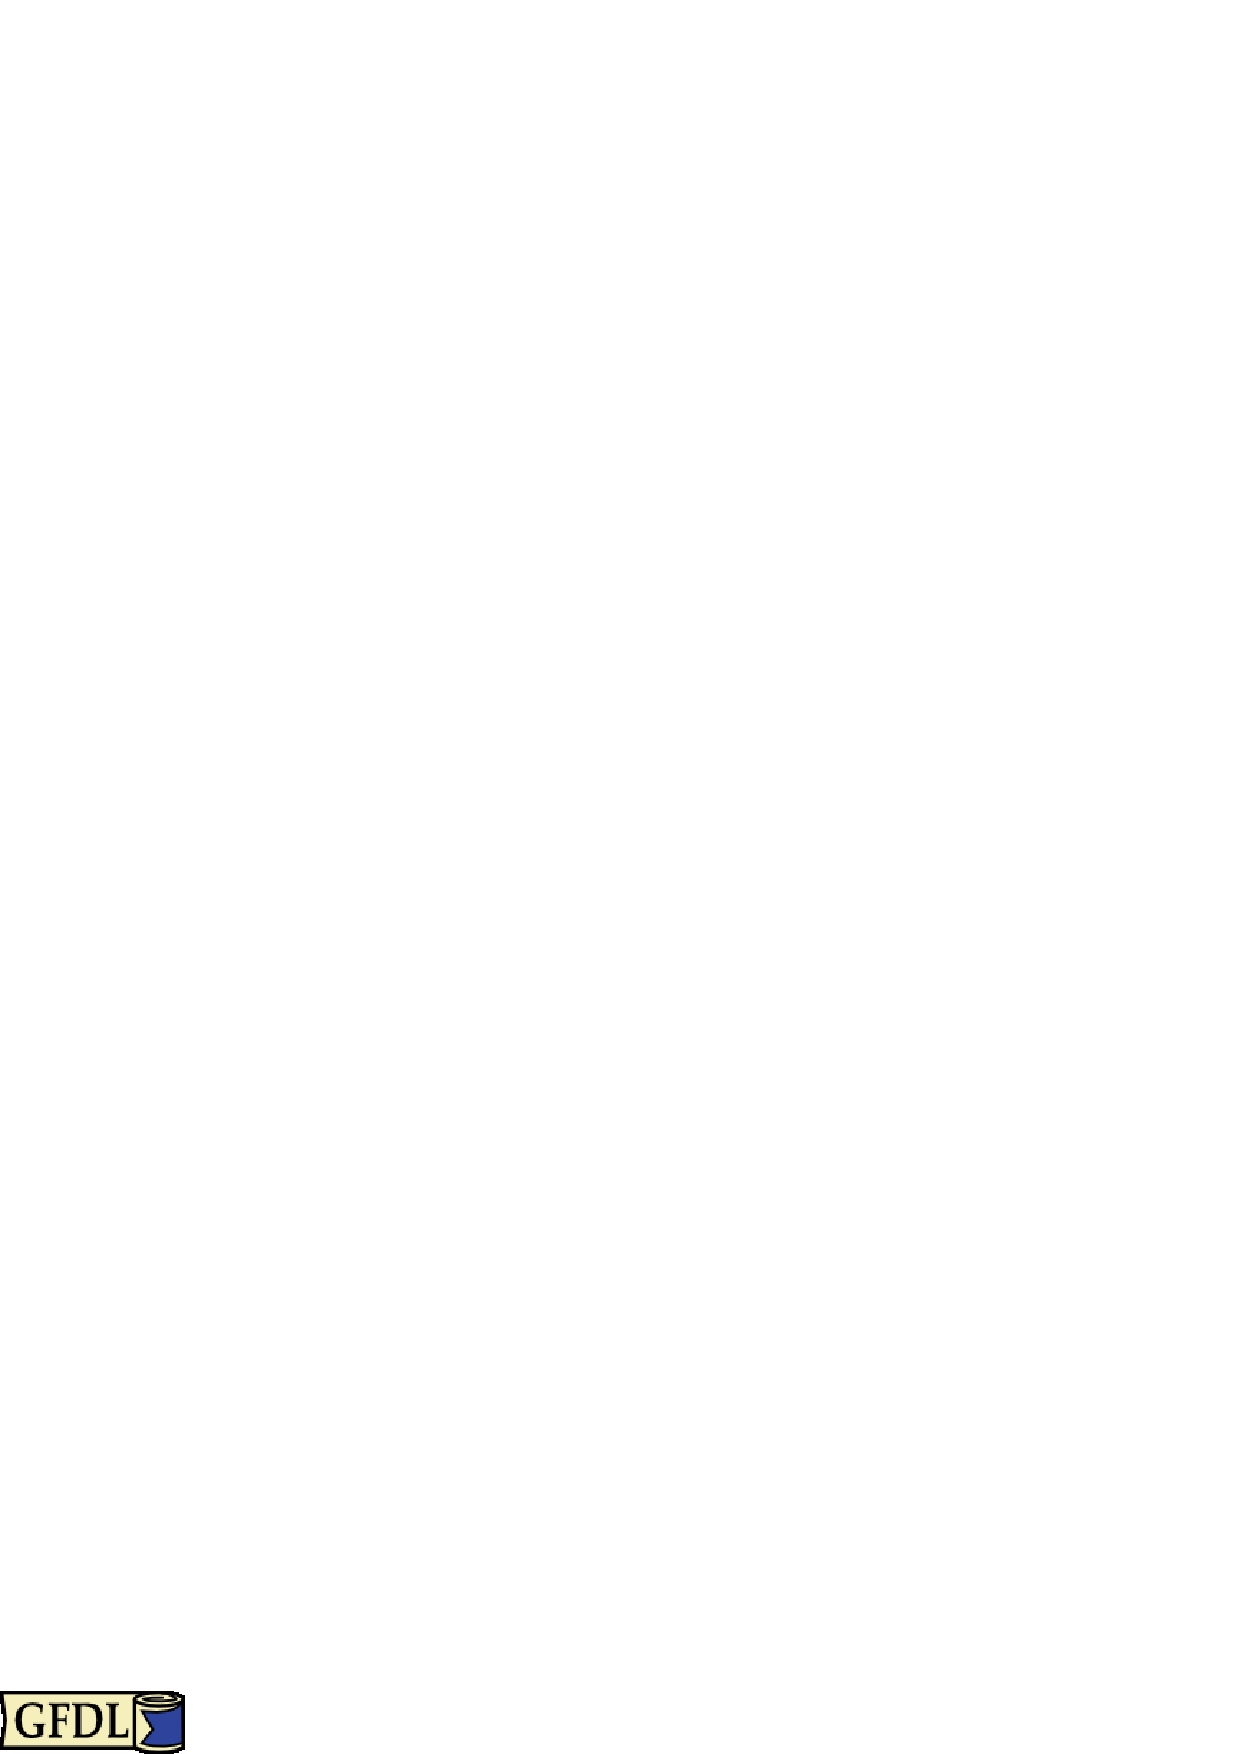
\includegraphics[width=1cm]{gfdl-logo-small.png}
        \else
            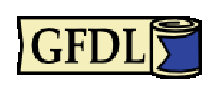
\includegraphics[width=1cm]{gfdl-logo-small.eps}
        \fi

Copyright (c) 2012  Laurent Claessens

Permission is granted to copy, distribute and/or modify this document under the terms of the \href{http://www.gnu.org/licenses/fdl-1.3.html}{GNU Free Documentation License}, Version 1.3 or any later version published by the Free Software Foundation; with no Invariant Sections, no Front-Cover Texts, and no Back-Cover Texts. A copy of the license is included in the chapter entitled ``GNU Free Documentation~License''.

\vspace{0.5cm}

Vous avez le droit de copier, distribuer et modifier ce document pourvu que vous suiviez les règles de la \wikipedia{fr}{GFDL}{GNU Free Documentation License}. Vous trouverez les sources \LaTeX\ sur gitorious :\\
    \url{https://www.gitorious.org/smath/smath/trees/master}

\end{center}


\newpage

% This is part of Un soupçon de mathématique sans être agressif pour autant
% Copyright (c) 2012
%   Laurent Claessens
% See the file fdl-1.3.txt for copying conditions.

%+++++++++++++++++++++++++++++++++++++++++++++++++++++++++++++++++++++++++++++++++++++++++++++++++++++++++++++++++++++++++++
\section*{Introduction}
%+++++++++++++++++++++++++++++++++++++++++++++++++++++++++++++++++++++++++++++++++++++++++++++++++++++++++++++++++++++++++++

Ces notes sont rédigées pour mes classes de seconde, de première STMG et de terminale STL du lycée Jacques Duhamel.

Pour la partie statistiques, j'ai pompé énormément à Pauline Klein\footnote{Je tiens à préciser que sa mise en page était plus belle que celle que celle que vous trouverez ici.}.

Les exercices ont profité des exemples donnés par madame Colette Perrot (merci) et des fiches \cite{qyKnLf} sur les statistiques descriptives trouvées sur le site de l'université de Montpelier 3 (Paul Valéry). Je les copie ici avec l'aimable autorisation de Richard Varro.



\tableofcontents

\newpage

%&=& &=& &=& &=& &=& &=& &=& &=& &=& &=& &=& &=& &=& &=& &=& &=& &=& &=& &=& &=& &=& &=& &=& 
\part{Seconde}
%&=& &=& &=& &=& &=& &=& &=& &=& &=& &=& &=& &=& &=& &=& &=& &=& &=& &=& &=& &=& &=& &=& &=& 

\chapter{Repères, distances, milieux}
% This is part of Un soupçon de mathématique sans être agressif pour autant
% Copyright (c) 2012-2013
%   Laurent Claessens
% See the file fdl-1.3.txt for copying conditions.


%+++++++++++++++++++++++++++++++++++++++++++++++++++++++++++++++++++++++++++++++++++++++++++++++++++++++++++++++++++++++++++
\section{Repères et coordonnées}
%+++++++++++++++++++++++++++++++++++++++++++++++++++++++++++++++++++++++++++++++++++++++++++++++++++++++++++++++++++++++++++

%AFAIRE : installer geogebra.


Début de match sur un terrain faisant \unit{50}{\meter} de large et \unit{100}{\meter} de long. Le joueur \( A\) fait une passe à son attaquant \( B\). Ce dernier est situé \unit{10}{\meter} au-dessus de la ligne médiane et à \unit{5}{\meter} à gauche du bord du terrain.

\begin{center}
   \input{Fig_EGDFJAT.pstricks}
\end{center}

\begin{enumerate}
    \item
        Compléter le dessin.
    \item
        Quelle est la longueur de la passe ?
    \item
        L'attaquant veut directement tirer vers le but. À quelle distance est-il ?
\end{enumerate}
% Le rayon du cercle au centre est de 10m, mais c'est fait exprès que c'est pas donné.


\begin{definition}
    Un \defe{repère orthonormé}{repère!orthonormé} du plan est la donné de trois points \( O\), \( I\), \( J\) non alignés formant un triangle rectangle isocèle en  \( O\).
\end{definition}

\begin{definition}
    Un \defe{repère}{repère} (quelconque) du plan est la donnée de trois points \( (O,I,J)\) non alignés.

    Les deux axes sont les droites \( (OI)\) et \( (OJ)\). Les longueurs \( OI\) et \( OJ\) servent de graduation.
\end{definition}

%+++++++++++++++++++++++++++++++++++++++++++++++++++++++++++++++++++++++++++++++++++++++++++++++++++++++++++++++++++++++++++
\section{Distance entre deux points}
%+++++++++++++++++++++++++++++++++++++++++++++++++++++++++++++++++++++++++++++++++++++++++++++++++++++++++++++++++++++++++++

\begin{Aretenir}

\begin{wrapfigure}{r}{7.0cm}
   \vspace{-1.5cm}        % à adapter.
   \centering
   \input{Fig_PythagoreeBqLDU.pstricks}
\end{wrapfigure}

        Soient les points \( A\) et \( B\) de coordonnées \( A=(x_A,y_A)\) et \( B=(x_B,y_B)\) dans un repère orthonormé. La distance entre \( A\) et \( B\) est donnée par la formule
        \begin{equation*}
            AB =\sqrt{(x_B-x_A)^2+(y_B-y_A)^2}.
        \end{equation*}
    \end{Aretenir}

% Attention : cette démonstration n'est pas du tout à donner en classe. On met seulement l'illustration.
\begin{proof}
    Nous allons utiliser le théorème de Pythagore. Pour cela nous construisons le triangle rectangle construit sur les points \( A\) et \( B\) comme indiqué sur le dessin. Le point \( C\) est le point de même abscisse que \( B\) et de même ordonnée que \( A\), c'est à dire que \( C\) est le point
    \begin{equation}
        C=(x_B,y_A).
    \end{equation}
    La droite \( AC\) est parallèle à l'axe des abscisses et la droite \( BC\) est parallèle à l'axe des ordonnées; elles sont donc perpendiculaires et le triangle \( ABC\) est un triangle rectangle en \( C\). Le théorème de Pythagore s'applique :
    \begin{equation}    \label{EqjLjEKr}
       AB =\sqrt{ AC^2+BC^2}.
    \end{equation}
    Il reste à déterminer les longueurs \(  AC \) et \(  BC \). Le segment \( [AC]\) est horizontal et s'étend de l'abscisse \( x_A\) à l'abscisse \( x_B\), donc il est de longueur soit \( x_A-x_B\) soit \( x_B-x_A\), mais dans les deux cas nous avons
    \begin{equation}
         AC^2=(x_B-x_A)^2.
    \end{equation}
    De la même façon nous avons 
    \begin{equation}
         BC^2=(y_B-y_A)^2.
    \end{equation}
    En remplaçant dans \eqref{EqjLjEKr}, nous obtenons le résultat annoncé.
\end{proof}

%+++++++++++++++++++++++++++++++++++++++++++++++++++++++++++++++++++++++++++++++++++++++++++++++++++++++++++++++++++++++++++
\section{Milieu d'un segment}
%+++++++++++++++++++++++++++++++++++++++++++++++++++++++++++++++++++++++++++++++++++++++++++++++++++++++++++++++++++++++++++

\begin{Aretenir}
    Soient les points \( A\) et \( B\) de coordonnées \( A=(x_A;y_A)\) et \( B=(x_B;y_B)\) dans un repère. Alors le milieu du segment \( [AB]\) est le point de coordonnées
    \begin{equation*}
            \left( \frac{ x_A+x_B }{ 2 }\,;\,\frac{ y_A+y_B }{2} \right).
    \end{equation*}
\end{Aretenir}


%+++++++++++++++++++++++++++++++++++++++++++++++++++++++++++++++++++++++++++++++++++++++++++++++++++++++++++++++++++++++++++
\section{Compléments}
%+++++++++++++++++++++++++++++++++++++++++++++++++++++++++++++++++++++++++++++++++++++++++++++++++++++++++++++++++++++++++++

La façon dont nous associons à chaque point \( M\) du plan ses coordonnées dans le repère \( O\), \( I\), \( J\) est donnée à la figure \ref{LabelFigReperexjVyii}.
\newcommand{\CaptionFigReperexjVyii}{Lire les coordonnées du point \( M\) dans le repère \( OIJ\).}
\input{Fig_ReperexjVyii.pstricks}

%+++++++++++++++++++++++++++++++++++++++++++++++++++++++++++++++++++++++++++++++++++++++++++++++++++++++++++++++++++++++++++ 
\section{Exercices supplémentaires}
%+++++++++++++++++++++++++++++++++++++++++++++++++++++++++++++++++++++++++++++++++++++++++++++++++++++++++++++++++++++++++++


\Exo{smath-0021}
\Exo{smath-0028}
\Exo{Seconde-0100}
\Exo{Seconde-0085}
\Exo{Seconde-0083}
\Exo{Seconde-0003}
\Exo{Seconde-0084}
\Exo{Seconde-0099}
\Exo{Seconde-0013}
\Exo{Seconde-0021}
\Exo{Seconde-0019} % Celui-ci contient un coefficient directeur et une équation de droite.
\Exo{Seconde-0079}
\Exo{Seconde-0080}
\Exo{Seconde-0078}
\Exo{smath-0029}
\Exo{Seconde-0081}
\Exo{smath-0124}
\Exo{Seconde-0077}
\Exo{smath-0027}
\Exo{Seconde-0082}
\Exo{Seconde-0001}
\Exo{Seconde-0062}
\Exo{smath-0026}


\chapter{Fonctions : mode graphique}
%This is part of Un soupçon de mathématique sans être agressif pour autant
% Copyright (c) 2012-2013
%   Laurent Claessens
% See the file fdl-1.3.txt for copying conditions.

%+++++++++++++++++++++++++++++++++++++++++++++++++++++++++++++++++++++++++++++++++++++++++++++++++++++++++++++++++++++++++++ 
\section{Objectifs du chapitre}
%+++++++++++++++++++++++++++++++++++++++++++++++++++++++++++++++++++++++++++++++++++++++++++++++++++++++++++++++++++++++++++

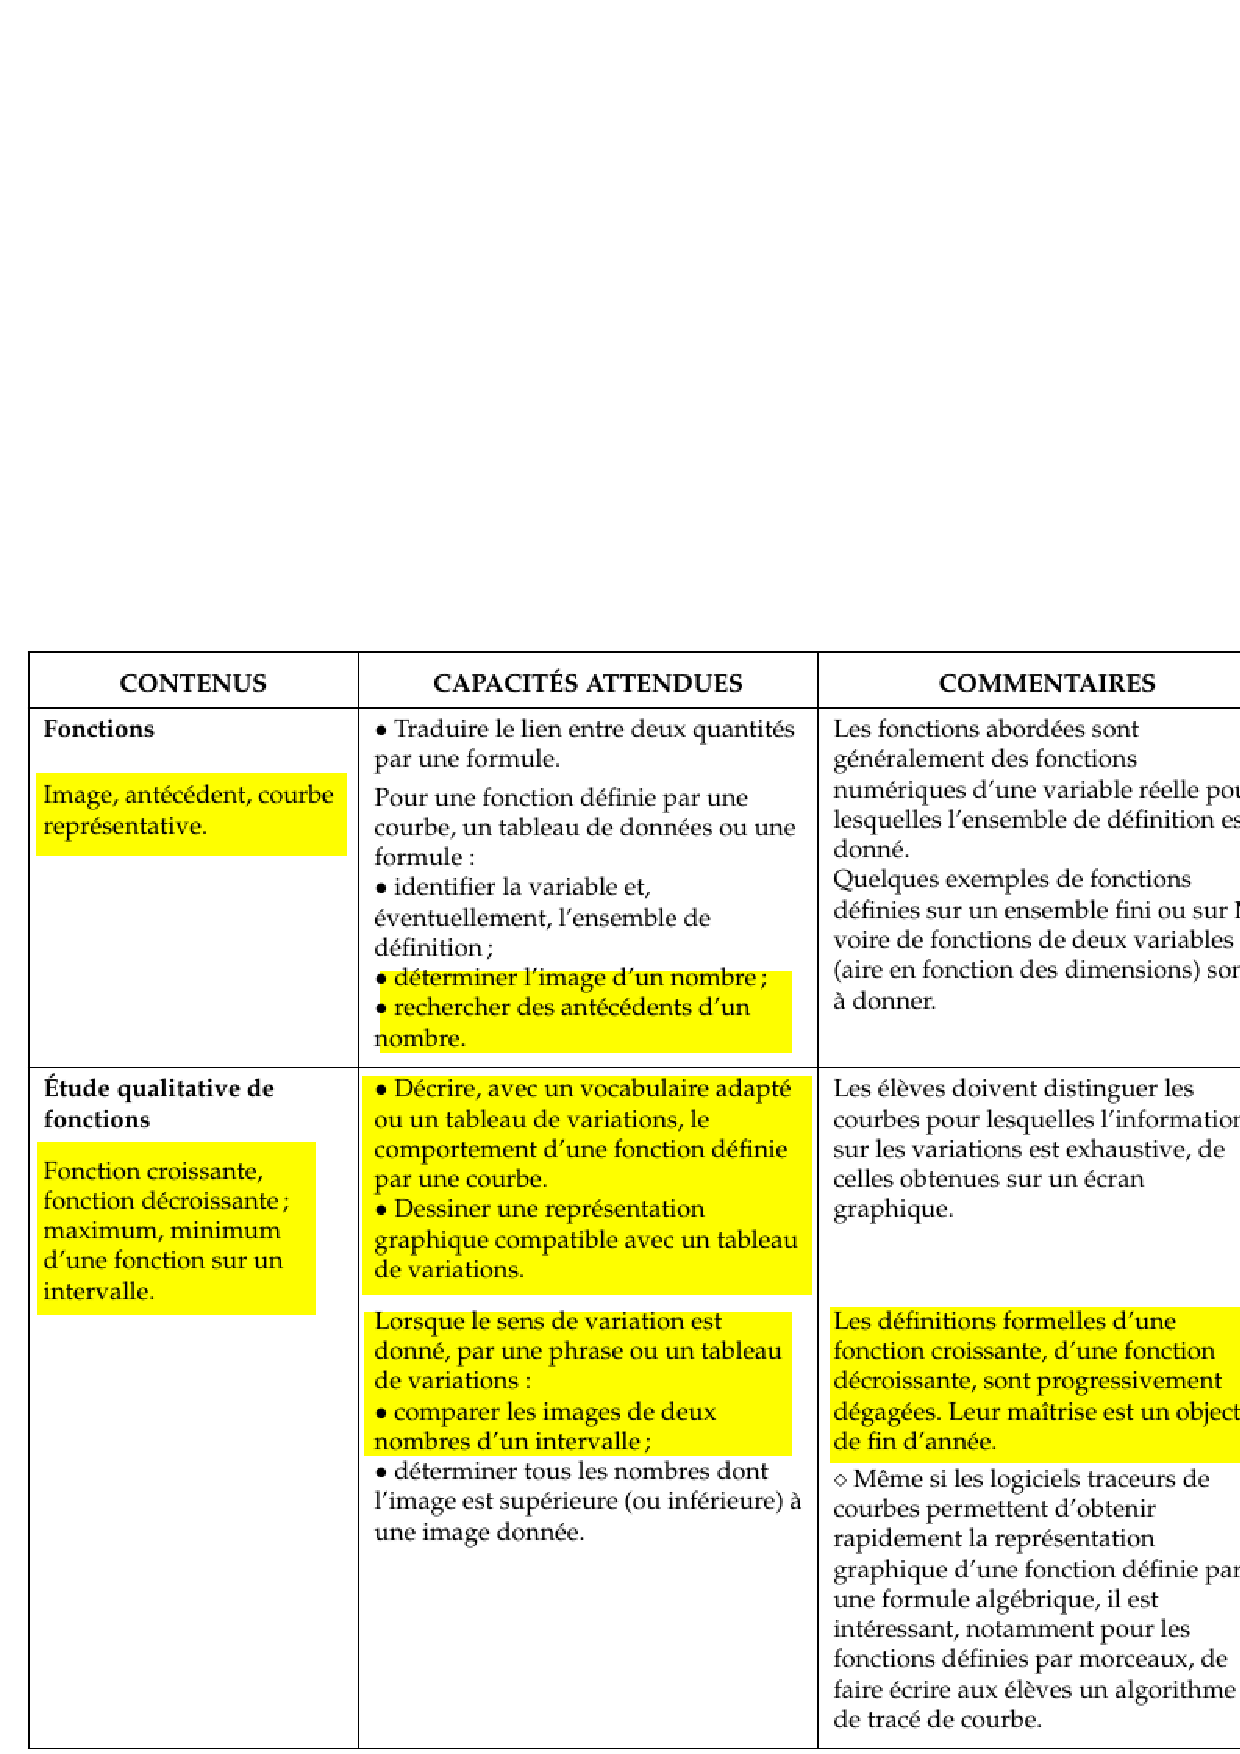
\includegraphics[width=\linewidth]{BO_fonctions_graphique.png}

%+++++++++++++++++++++++++++++++++++++++++++++++++++++++++++++++++++++++++++++++++++++++++++++++++++++++++++++++++++++++++++
\section{Courbe représentative d'une fonction}
%+++++++++++++++++++++++++++++++++++++++++++++++++++++++++++++++++++++++++++++++++++++++++++++++++++++++++++++++++++++++++++

% Partie graphique du berger syldave.
\begin{Aprojeter}
    %This is part of Un soupçon de mathématique sans être agressif pour autant
% Copyright (c) 2012-2013
%   Laurent Claessens
% See the file fdl-1.3.txt for copying conditions.

    Un berger syldave s'entraine pour le championnat national du lancer de chèvre. L'épreuve consiste à lancer une chèvre vers le haut depuis le bord d'une falaise située au bord d'un lac tranquille. La hauteur de la chèvre en fonction du temps par rapport à la surface du lac tranquille est une fonction \( f\) donnée par le graphique suivant.

    \begin{center}
        \input{Fig_WRXbDCo.pstricks}
    \end{center}
    La dernière partie du graphique correspond à la chèvre que l'on remonte rapidement hors de l'eau.
    À partir du graphique :
    \begin{enumerate}
        \item
            À quelle hauteur se trouve la chèvre au moment du lancer ?
        \item
            Pendant combien de temps la chèvre reste à une hauteur supérieure à celle à laquelle elle a été lancée ?
        \item
            À quel moment la chèvre atteint-elle sa hauteur maximale ? Quelle est cette hauteur ?
        \item
            À quelle hauteur se trouve la chèvre après \( 2.5\) secondes de vol ?
        \item
            Résumer toutes ces informations en dressant le tableau de variation de la fonction \( f\).
    \end{enumerate}

\end{Aprojeter}

\begin{definition}
Soit $f$ une fonction définie sur un ensemble $\defD$.
    On appelle \defe{représentation graphique}{représentation graphique (d'une fonction)}, ou le \defe{graphe}{graphe} de $f$, l'ensemble des points $(x,y)$ tels que $x\in\defD$ et $y=f(x)$.

    Lorsque \( y=f(x)\), le nombre \( y\) est l'\defe{image}{image par une fonction} de \( x\) par la fonction \( f\) et \( x\) est \emph{un} \defe{antécédent}{antécédent} de \( y\).
\end{definition}

\begin{Aretenir}
    La règle d'or des graphiques : le point de coordonnées \( (a;b)\) est sur le graphique de la fonction \( f\) si et seulement si \( f(a)=b\).
\end{Aretenir}

\begin{multicols}{2}

À propos du graphe ci-contre :
\begin{enumerate}
    \item
        Quel est l'ensemble de définition de la fonction \( f\) ?
    \item
        Quelle est l'image de \( 1\) par \( f\) ?
    \item
        Donner un antécédent de \( 3\).
    \item
        Que vaut \( f(-3)\) ?
    \item
        Quels sont les antécédents de \( -1\) ?
    \item 
        Quel est le maximum de \( f\) sur \( \mathopen[ -2 , 1 \mathclose]\) ?
    \item
        Quel est le maximum de \( f\) sur \( \mathopen[ -2 , 2 \mathclose]\) ?
\end{enumerate}
    
    \columnbreak

\begin{center}
   \input{Fig_AHAbqhj.pstricks}
\end{center}

\end{multicols}


%+++++++++++++++++++++++++++++++++++++++++++++++++++++++++++++++++++++++++++++++++++++++++++++++++++++++++++++++++++++++++++ 
    \section{Minimum et maximum}
%+++++++++++++++++++++++++++++++++++++++++++++++++++++++++++++++++++++++++++++++++++++++++++++++++++++++++++++++++++++++++++


Les notions de minima et maxima parlent, comme l'indiquent leurs noms en français, des points du graphe d'une fonction les plus hauts et les plus bas.

\begin{definition}
      Soit $f$ une fonction définie sur un intervalle \( I\).
      \begin{itemize}
            \item 
                Nous disons que le réel \( M\) est le \defe{maximum}{maximum} de \( f\) sur $I$ si et seulement si 
                \begin{enumerate}
                    \item
                        il existe $ a\in I$ tel que $f(a)=M$,
                    \item
                        \( f(x)\leq M\) pour tout $x\in I$.
                \end{enumerate}
                
          \item 
                Nous disons que le réel \( m\) est le \defe{minimum}{minimum} de \( f\) sur $I$ si et seulement si
                \begin{enumerate}
                    \item
                        il existe $ b\in I$ tel que $f(b)=m$,
                    \item
                        $f(x)\geq m$ pour tout \( x\in I\).
                \end{enumerate}
      \end{itemize}
\end{definition}

\begin{wrapfigure}[9]{r}{7.0cm}
   \vspace{-0.5cm}        % à adapter.
   \centering
   \input{Fig_MinMaxKNRdOd.pstricks}
\end{wrapfigure}

\begin{remark}
    Attention à deux choses.
    \begin{enumerate}
        \item
            Le minimum est la \emph{valeur} la plus basse, et non l'abscisse correspondante. Idem pour le maximum. 
        \item
            La minimum dépend de l'intervalle sur lequel on regarde la fonction.
    \end{enumerate}
\end{remark}

Une illustration sur la figure ci-contre. La fonction prend son maximum en \( x=a\) et ce maximum vaut \( M\). La fonction prend son minimum en \( x=b\) et ce minimum vaut \( m\).


\chapter{Fonctions affines et linéaires}
%This is part of Un soupçon de mathématique sans être agressif pour autant
% Copyright (c) 2012-2013
%   Laurent Claessens
% See the file fdl-1.3.txt for copying conditions.

%+++++++++++++++++++++++++++++++++++++++++++++++++++++++++++++++++++++++++++++++++++++++++++++++++++++++++++++++++++++++++++ 
\section{Objectifs du chapitre}
%+++++++++++++++++++++++++++++++++++++++++++++++++++++++++++++++++++++++++++++++++++++++++++++++++++++++++++++++++++++++++++

Le but de ce chapitre est de voir la notion de fonction affine.
\begin{enumerate}
    \item
        La forme \( x\mapsto mx+p\).
    \item
        Représentation graphique : signe de \( m\), coefficient directeur et ordonnée à l'origine.
    \item
        Tableau de signe.
    \item
        Résolution des équations correspondantes.
\end{enumerate}
Nous ne parlerons pas d'équation de droite à proprement parler. Donc pas de graphes de fonctions passant par deux points donné.

\EpsOrPdfincludegraphics[width=\linewidth]{BO_fonctions_affines1.png}

\vspace{1cm}

\EpsOrPdfincludegraphics[width=\linewidth]{BO_fonctions_affines2.png}

%+++++++++++++++++++++++++++++++++++++++++++++++++++++++++++++++++++++++++++++++++++++++++++++++++++++++++++++++++++++++++++ 
\section{L'activité}
%+++++++++++++++++++++++++++++++++++++++++++++++++++++++++++++++++++++++++++++++++++++++++++++++++++++++++++++++++++++++++++

%This is part of Un soupçon de mathématique sans être agressif pour autant
% Copyright (c) 2012-2013
%   Laurent Claessens
% See the file fdl-1.3.txt for copying conditions.

    Le taxi Besacdanslesac divise son prix en deux parties : $0.2$ euros de frais de prise en charge plus un euro par km parcouru. Le taxi Ledoubstoudoux par contre divise son prix en $1$ euro de frais de prise en charge plus $0.8$ euros par kilomètre parcouru.

    \begin{enumerate}
        \item
            Combien coûte un trajet de \SI{5}{\kilo\meter} avec Besacdanslesac ?
        \item
            Donner une expression algébrique du prix d'une course en fonction du nombre de kilomètres parcourus.
        \item
            Combien de kilomètres peut-t-on effectuer dans Ledoubstoudoux avec \( 10\) euros ?
        \item
            Exprimer les prix en fonction du nombre de kilomètres parcourus sur un graphique (les deux taxis sur le même graphique).
        \item
            À partir de combien de kilomètres parcourus vaut-il mieux prendre Ledoubstoudoux ?
    \end{enumerate}



%+++++++++++++++++++++++++++++++++++++++++++++++++++++++++++++++++++++++++++++++++++++++++++++++++++++++++++++++++++++++++++ 
\section{Définitions}
%+++++++++++++++++++++++++++++++++++++++++++++++++++++++++++++++++++++++++++++++++++++++++++++++++++++++++++++++++++++++++++

\begin{definition}
    Une \defe{fonction affine}{affine}\index{fonction!affine} est une fonction définie sur \( \eR\) par
    \begin{equation}
        f(x)=mx+p
    \end{equation}
    où \( m\) et \( p\) sont deux nombres réels fixés.
\end{definition}

%+++++++++++++++++++++++++++++++++++++++++++++++++++++++++++++++++++++++++++++++++++++++++++++++++++++++++++++++++++++++++++ 
\section{Tracer la droite représentative de la courbe}
%+++++++++++++++++++++++++++++++++++++++++++++++++++++++++++++++++++++++++++++++++++++++++++++++++++++++++++++++++++++++++++

Nous savons depuis la classe de troisième que la représentation graphique d'une fonction affine est une droite. Une question qui vient immédiatement est : comment la tracer ?

En principe ça a déjà été inventé pour le problème des taxis.


\begin{example}
    \begin{wrapfigure}[20]{r}{7.0cm}
   \vspace{-0.5cm}        % à adapter.
   \centering
   \input{Fig_OWGRRSC.pstricks}
\end{wrapfigure}

    Prenons la fonction \( f(x)=3x+2\). Si on pense en termes de taxi, c'est un taxi qui demande \( 3\) euros par kilomètres et \( 2\) euros. Il demande donc \( 5\) euros pour \unit{1}{\kilo\meter}, \( 11\) euros pour \unit{3}{\kilo\meter} etc. Il suffit de faire le graphe de cela. 

    % Attention : les nombres de km de ce texte sont codés en dur dans le fichier phystricksOWGRRSC

    On fait quelque points, puis on trace avec une règle.

    Attention : il faut bien prolonger la droite également vers les négatifs, sauf si le contexte interdit les nombres négatifs.
    
\end{example}

%+++++++++++++++++++++++++++++++++++++++++++++++++++++++++++++++++++++++++++++++++++++++++++++++++++++++++++++++++++++++++++ 
\section{Terminologie}
%+++++++++++++++++++++++++++++++++++++++++++++++++++++++++++++++++++++++++++++++++++++++++++++++++++++++++++++++++++++++++++

\begin{Aretenir}
    Le graphe de la fonction \( x\mapsto mx+p\) passe par le point de coordonnées \( (0;p)\).
    \begin{enumerate}
        \item
            \( p\) est l'\defe{ordonnées à l'origine}{ordonnées!à l'origine} de la fonction affine \( mx+p\).
        \item
            \( m\) est le \defe{coefficient directeur}{coefficient directeur} de la fonction affine \( mx+p\).
    \end{enumerate}
\end{Aretenir}

Cas particuliers :
\begin{enumerate}
    \item
        Si \( p=0\) alors \( f(x)=mx\) et nous disons que \( f\) est une fonction \defe{linéaire}{fonction!linéaire}. Son graphe passe par l'origine \( (0;0)\).
    \item
        Si \( m=0\) alors \( f(x)=p\) et nous disons que \( f\) est une fonction \defe{constante}{fonction!constante}.
\end{enumerate}

%+++++++++++++++++++++++++++++++++++++++++++++++++++++++++++++++++++++++++++++++++++++++++++++++++++++++++++++++++++++++++++ 
\section{Représentation graphique}
%+++++++++++++++++++++++++++++++++++++++++++++++++++++++++++++++++++++++++++++++++++++++++++++++++++++++++++++++++++++++++++

\begin{Aretenir}
    La représentation graphique de la fonction \( f(x)=mx+p\) est une droite non parallèle à l'axe des ordonnées. Réciproquement toute droite non parallèle est la représentation graphique d'une fonction affine.
\end{Aretenir}


Un exemple des éléments de \( mx+p\) est donné à la figure \ref{LabelFigfigureUERGVgS}. % From file figureUERGVgS
La droite «commence» à la hauteur \( p\) et ensuite monte encore de \( m\) vers le haut à chaque pas de \( 1\) vers la droite.
\newcommand{\CaptionFigfigureUERGVgS}{Une droite et quelque éléments de son équation.}
\input{Fig_figureUERGVgS.pstricks}

\begin{Aretenir}
    Soit \( f\) la fonction affine \( x\mapsto mx+p\).
    \begin{enumerate}
        \item
            Si \( m>0\) alors \( f\) est croissante sur \( \eR\).
        \item
            Si \( m<0\) alors \( f\) est décroissante sur \( \eR\).
        \item
            Si \( m=0\) alors \( f\) est constante sur \( \eR\) (et vaut \( p\)).
    \end{enumerate}
\end{Aretenir}

%--------------------------------------------------------------------------------------------------------------------------- 
\subsection{Tableau de signe d'une fonction affine}
%---------------------------------------------------------------------------------------------------------------------------

Nous savons qu'une fonction affine est croissante ou décroissante suivant le signe de \( m\). Il y a donc deux tableaux de signes possibles.

\begin{minipage}{0.485\textwidth}
    \begin{center}

        Si \( m<0\)
        \vspace{5mm}

               \input{Fig_OSQOqJN.pstricks}   

               \begin{equation*}
                   \begin{array}[]{c|ccccc}
                       x&-\infty&&-\frac{ p }{ m }&&\infty\\
                         \hline
                         mx+p&&-&0&+&\\ 
                          \end{array}
                      \end{equation*}
    \end{center}
\end{minipage}
\hspace{1mm}
\begin{minipage}{0.485\textwidth}
    \begin{center}
        Si \( m>0\)
        \vspace{5mm}

                    \input{Fig_BZqEWco.pstricks}

               \begin{equation*}
                   \begin{array}[]{c|ccccc}
                       x&-\infty&&-\frac{ p }{ m }&&\infty\\
                         \hline
                         mx+p&&+&0&-&\\ 
                          \end{array}
                      \end{equation*}
    \end{center}
\end{minipage}


\chapter{Statistique descriptive}
% This is part of Un soupçon de mathématique sans être agressif pour autant
% Copyright (c) 2012-2013
%   Laurent Claessens, Pauline Klein
% See the file fdl-1.3.txt for copying conditions.


\EpsOrPdfincludegraphics[width=\linewidth]{BO_statistique_descriptive}


\setcounter{section}{-1}
%+++++++++++++++++++++++++++++++++++++++++++++++++++++++++++++++++++++++++++++++++++++++++++++++++++++++++++++++++++++++++++ 
\section{Activité : un peu de spam ?}
%+++++++++++++++++++++++++++++++++++++++++++++++++++++++++++++++++++++++++++++++++++++++++++++++++++++++++++++++++++++++++++

% This is part of Un soupçon de mathématique sans être agressif pour autant
% Copyright (c) 2013
%   Laurent Claessens
% See the file fdl-1.3.txt for copying conditions.

% ATTENTION : les chiffres donnés ici sont repris dans le cours au moment des ECC.
% ATTENTION : il y a trop de 4 dans les valeurs, les effectifs et les ECC. Il faut changer.
%               Il faut changer au moins dans le texte ici, dans la figure et dans le texte des éléments de réponse.

\begin{wrapfigure}[5]{r}{8cm}
   \vspace{-0.5cm}        % à adapter.
   \centering
   \input{Fig_YRQOoPE.pstricks}
\end{wrapfigure}

Le graphique ci-contre illustre le nombre de spam reçus aujourd'hui par les élèves d'une classe.
\begin{enumerate}
    \item
        Combien d'élèves y-a-t-il dans la classe ?
    \item
        Combien d'élèves ont reçu \( 5\) spams ou plus ?
    \item
        En moyenne combien de spam ont reçu les élèves aujourd'hui ?
    \item
        Diviser la classe en 4 groupes suivant le nombre de spams reçus.
\end{enumerate}



Éléments de réponse.

\begin{enumerate}
    \item
Nous pouvons remplir le tableau
\begin{equation*}
    \begin{array}[]{|c||c|c|c|c|c|c|c|c|c|c|c|| c |}
        \hline
        \text{Nombre}&1&2&3&4&5&6&7&8&9&10&11&\text{total}\\
        \hline\hline
        \text{Effectifs}&3&0&1&4&4&2&1&5&3&1&1&25\\
        \hline
    \end{array}
\end{equation*}
\item
Il y a \( 17\) élèves ayant reçu \( 5\) spams ou plus.
     \item
         Pour calculer la moyenne il faut d'abord calculer le nombre total de spams reçus, puis diviser par le nombre d'élèves :
         \begin{equation}
             \text{moyenne}=\frac{ 3\times 1+1\times 3+4\times 4+4\times 5+2\times 6+\ldots+1\times 11 }{ 25 }=\frac{ 149 }{ 25 }=5.96.            
         \end{equation}
     \item
         En ce qui concerne la division de la classe en quatre groupe, vu que \( 25\) n'est pas divisible en \( 4\), il va falloir donner une convention sur les arrondis.
\end{enumerate}

%+++++++++++++++++++++++++++++++++++++++++++++++++++++++++++++++++++++++++++++++++++++++++++++++++++++++++++++++++++++++++++ 
\section{Convention sur les quartiles et médiane}
%+++++++++++++++++++++++++++++++++++++++++++++++++++++++++++++++++++++++++++++++++++++++++++++++++++++++++++++++++++++++++++

\begin{definition}
    Nous considérons une liste de \( n\) valeurs triées par ordre croissant (avec éventuellement les répétitions).
    \begin{enumerate}
        \item
            La \defe{médiane}{médiane}, est la valeur qui sépare la liste en deux parties égales. C'est le terme du milieu si l'effectif total est impair et la moyenne des deux termes du milieu si l'effectif total est pair.
      \item 
          Le \defe{premier quartile}{quartile!premier} $Q_1$ est la plus petite valeur de la liste telle qu'au moins un quart des valeurs de la liste soient inférieures ou égales à $Q_1$.
        \item
            Le \defe{troisième quartile}{quartile!troisième} $Q_3$ est la plus petite valeur de la liste telle qu'au moins les trois quarts des valeurs de la liste soient inférieures ou égales à $Q_3$.
  \end{enumerate}
\end{definition}
En pratique :
\begin{itemize}
    \item 
  Pour le calcul de $Q_1$, on calcule $\dfrac{n}4$, puis on détermine le premier entier $p$ supérieur ou égal à $\dfrac{n}4$. Cet entier $p$ donne le rang de $Q_1$. 
  \item
  Pour le calcul de $Q_3$, on fait de même en remplaçant $\dfrac{n}4$ par $\dfrac{3n}4$. 
\end{itemize}


\begin{example}

    Un laboratoire expérimente un médicament sur dix souris. Voici les temps (en semaines) que les souris ont encore vécu après l'injection : \( 2\), \( 5\), \( 10\), \( 2\), \( 1\), \( 3\), \( 10\), \( 5\), \( 5\), \( 1\).

    D'abord nous trions par ordre croissant en respectant les répétitions :
    \begin{equation*}
        \begin{array}[]{|c||c|c|c|c|c|c|c|c|c|c|}
            \hline
            \text{numéro de la souris}&1&2&3&4&5&6&7&8&9&10\\
            \hline
            \text{semaines de vie}&1&1&2&2&3&5&5&5&10&10\\
            \hline
        \end{array}
    \end{equation*}

    Il y a \( 10\) valeurs, donc 
    \begin{enumerate}
        \item
            Pour le premier quartile, \( \frac{ 10 }{ 4 }\simeq 2.5\), on prend la troisième valeur : \( Q_1=2\).
        \item
            Pour le troisième quartile, \( \frac{ 3}{ 4 }\times 10\simeq 7.5\), on prend la huitième valeur : \( Q_3=5\).
        \item
            Pour la médiane, on prend la moyenne entre la cinquième et la sixième valeur : \( \frac{ 3+5 }{2}=4\) : \( Med=4\).
    \end{enumerate}

    Nous résumons ces informations sur le diagramme suivant :


    \begin{center}
        \input{Fig_DNYAefI.pstricks}
    \end{center}


    Attention : nouvelle de dernière minute. Le laboratoire s'est trompé dans ses résultats. En réalité les deux souris qui ont vécu \( 10\) semaines ont vécu respectivement \( 15\) et \( 20\) semaines. Est-ce que ça change quelque chose ?

\end{example}

Les conventions sur les quartiles sont résumées ici :

\begin{center}
   \input{Fig_KDtwIJf.pstricks}
\end{center}

\section{Représentation graphique d'une série statistique}

%--------------------------------------------------------------------------------------------------------------------------- 
\subsection{Effectifs cumulés croissants}
%---------------------------------------------------------------------------------------------------------------------------

Nous classons les élèves d'une classe d'après la première lettre de leur noms. Le résultat est le tableau
\begin{center}
\begin{tabular}[]{|c||c|c|c|c|c|c|c|c|c|c|c|c||c|}
        \hline
        Lettre&a&b&c&d&h&j&l&m&p&r&s&t&total\\
        \hline\hline
        Effectifs&4&8&9&2&2&1&1&2&2&1&1&2&35\\
        \hline
        ECC&4&12&21&23&25&26&27&29&31&32&33&35&\\
        \hline
\end{tabular}
\end{center}

\input{Fig_MAXkaGz.pstricks}

%--------------------------------------------------------------------------------------------------------------------------- 
\subsection{Graphe des fréquences cumulées croissantes}
%---------------------------------------------------------------------------------------------------------------------------

Nous reprenons l'exemple du spam
\begin{equation*}
    \begin{array}[]{|c||c|c|c|c|c|c|c|c|c|c|c|| c |}
        \hline
        \text{Nombre}&1&2&3&4&5&6&7&8&9&10&11&\text{total}\\
        \hline\hline
        \text{Effectifs}&3&0&1&4&4&2&1&5&3&1&1&25\\
        \hline
        \text{Fréquences}&0.12&0&0.04&0.16&0.16&0.08&0.04&0.2&0.12&0.04&0.04&1\\
        \hline
        \text{FCC}&0.12&0.12&0.16&0.32&0.48&0.56&0.6&0.8&0.92&0.96&1&\\
        \hline
    \end{array}
\end{equation*}

\begin{center}
\input{Fig_FWyrYhJ.pstricks}
\end{center}

%--------------------------------------------------------------------------------------------------------------------------- 
\subsection{Histogramme}
%---------------------------------------------------------------------------------------------------------------------------

Le tableau suivant donne la répartition des entreprises du secteur automobile en fonction de leur chiffre d'affaire (en millions d'euros).

\begin{center}
    \begin{tabular}{|c||c|c|c|c|c|c|}
        \hline
        chiffre d'affaire&moins de \( 0.25\)&\( \mathopen[ 0.25 ,0.5 [\)&$\mathopen[ 0.5;1  [$&$\mathopen[ 1 , 2.5 [$&$\mathopen[ 2.5;5 ,  [$&$\mathopen[ 5 , 10 [$\\
            \hline\hline
            nombre d'entreprises&\( 137\)&\( 106\)&\( 112\)&$154$&\( 100\)&\( 33\)\\
            \hline
    \end{tabular}
\end{center}

\begin{Aretenir}
Pour des données rassemblées en classes, l'\textbf{aire} du rectangle est proportionnelle à l'effectif (ou à la fréquence). 
\end{Aretenir}

Nous en dessinons l'histogramme suivant :
\begin{center}
   \input{Fig_LTenBUj.pstricks}
\end{center}


Consignes pour dessiner un histogramme :
\begin{enumerate}
    \item
        Trouver la plus haute boîte en calculant le rapport \( \frac{ \text{effectif} }{ \text{largeur} }\) pour chaque boîte.
    \item
        Se fixer une échelle pour que la plus haute boîte reste raisonnable : elle ne doit pas faire deux mètres de haut, ni un centimètre. Il faut viser environ \unit{10}{\centi\meter}.
    \item
        Tracer les boîtes.
    \item
        Mettre la graduation \emph{horizontale} en écrivant la légende correspondante.
    \item
        Ne pas mettre de graduation verticale en cas d'histogramme à pas non constant\footnote{C'est à dire ceux dont la largeur n'est pas la même pour toute les boîtes.}.
    \item
        Écrire l'effectif de la boîte au-dessus de la boîte.
    \item
        Éventuellement écrire l'unité de surface «un carreau= \ldots effectifs». Par exemple «un carreau = 50 entreprises», «un carreau = 15 personnes».
\end{enumerate}



\begin{example}
    Si nous avons un effectif de \( 25\) personnes, un quart des effectifs seraient \( 6.25\) personnes, et les trois quarts seraient \( 18.75\) personnes. Donc nous mettons les premier quartile sur la \( 7\Ieme\) personne et le troisième quartile sur la \( 19\Ieme\) personne.

    Le premier quart des effectifs seraient donc les personnes numéro \( 1\), \( 2\), \( 3\), \( 4\), \( 5\), \( 6\) et \( 7\). Et le dernier quart des personnes seront les personnes numéro \( 20\), \( 21\), \( 22\), \( 23\), \( 24\) et \( 25\).
\end{example}


\chapter{Géométrie dans l'espace}
% This is part of Un soupçon de mathématique sans être agressif pour autant
% Copyright (c) 2012-2013
%   Laurent Claessens
% See the file fdl-1.3.txt for copying conditions.

\EpsOrPdfincludegraphics[width=\linewidth]{BO_perspective}

Note : savoir si deux droites dans l'espace sont perpendiculaires n'est pas au programme. Dans ce chapitre nous allons donc nous en tenir qu'à des choses simples.

\vspace{1cm}

% This is part of Un soupçon de mathématique sans être agressif pour autant
% Copyright (c) 2013
%   Laurent Claessens
% See the file fdl-1.3.txt for copying conditions.

\begin{wrapfigure}[3]{r}{5.0cm}
   \vspace{-0.5cm}        % à adapter.
   \centering
   \input{Fig_MEzTDZC.pstricks}
\end{wrapfigure}

À l'aide du cube ci-contre :
\begin{enumerate}
    \item
        Quelle est la nature du triangle \( AEF\) ? 
    \item
        Quelle est la nature du quadrilatère \( ABGH\) ?
    \item
        Est-ce que vous pouvez trouver trois points de ce cube formant un triangle équilatéral ?
    \item
        Si ce cube fait \unit{5}{\meter} de côté, quelle est la longueur de la «grande» diagonale \( [AG]\) ?
\end{enumerate}



%+++++++++++++++++++++++++++++++++++++++++++++++++++++++++++++++++++++++++++++++++++++++++++++++++++++++++++++++++++++++++++ 
\section{Ce qui est dans un plan}
%+++++++++++++++++++++++++++++++++++++++++++++++++++++++++++++++++++++++++++++++++++++++++++++++++++++++++++++++++++++++++++

Les trois suivantes permettent d'affirmer que tel point ou telle droite est dans un plan.
\begin{enumerate}
    \item
        Si \( d\) est une droite et \( P\) est un point d'un plan, alors la parallèle à \( d\) passant par \( P\) est encore dans le plan.
    \item
        Si \( P\) et \( Q\) sont deux points d'un plan, alors toute la droite \( (PQ)\) est encore dans ce plan.
    \item
        Deux droites non parallèles situées dans un même plan sont sécantes.
\end{enumerate}

%---------------------------------------------------------------------------------------------------------------------------
\subsection{Position relative de deux plans}
%---------------------------------------------------------------------------------------------------------------------------

\begin{definition}
    Deux plans sont \defe{parallèles}{parallèle!deux plans} soit si ils sont confondus, soit si ils n'ont aucun point commun. Si ils n'ont aucun point communs, nous disons qu'ils sont \defe{strictement parallèles}{parallèle!strictement}
\end{definition}


\begin{Aretenir}
    Deux plans non parallèles se coupent en une droite.
\end{Aretenir}

\begin{multicols}{2}

    \begin{center}
        Plans parallèles
    \end{center}
   % Des plans parallèles sont soit confondus, soit n'ont aucun point communs.
    

%Les plans \( (AEB)\) et \( (DHC)\) ci-contre sont parallèles.

\columnbreak

%The result is on figure \ref{LabelFigPositionPlansTvKvah}. % From file PositionPlansTvKvah
%\newcommand{\CaptionFigPositionPlansTvKvah}{<+Type your caption here+>}
    \begin{center}
\input{Fig_PositionPlansTvKvah.pstricks}
    \end{center}


\end{multicols}

\begin{multicols}{2}
    \begin{center}
        Plans sécants
    \end{center}
 %   L'intersection de deux plans sécants (non confondus) est une droite.

  %  L'intersection des plans \( (ABG)\) et \( (DCG)\) ci-contre est la droite \( (HG)\).

    \columnbreak

%The result is on figure \ref{LabelFigPositionPlansqSltxa}. % From file PositionPlansqSltxa
%\newcommand{\CaptionFigPositionPlansqSltxa}{<+Type your caption here+>}
    \begin{center}
\input{Fig_PositionPlansqSltxa.pstricks}
    \end{center}

\end{multicols}

%---------------------------------------------------------------------------------------------------------------------------
\subsection{Position relative de deux droites}
%---------------------------------------------------------------------------------------------------------------------------

Deux droites peuvent être soit dans un même plan, soit ne pas être dans le même plan. Deux droites contenues dans un même plan sont dires \defe{coplanaires}{coplanaire}.

%///////////////////////////////////////////////////////////////////////////////////////////////////////////////////////////
\subsubsection{Droites coplanaires}
%///////////////////////////////////////////////////////////////////////////////////////////////////////////////////////////

Deux droites coplanaires respectent la géométrie usuelle. Elles peuvent être parallèles ou sécantes.

\begin{multicols}{2}
    \begin{center}
        Droites parallèles dans le plan \( (EBC)\)
    \end{center}

    \columnbreak

    \begin{center}
        \input{Fig_IDqyzXM.pstricks}
    \end{center}
\end{multicols}

\begin{multicols}{2}
    \begin{center}
        Droites sécantes dans le plan \( (AEH)\)
    \end{center}

    \columnbreak

    \begin{center}
        \input{Fig_ETfnbsh.pstricks}
    \end{center}
\end{multicols}

\begin{Aretenir}
    À propos de droites coplanaires :
    \begin{enumerate}
        \item
            Deux droites sécantes sont toujours coplanaires.
        \item
            Deux droites parallèles sont coplanaires.
    \end{enumerate}
\end{Aretenir}

\begin{proof}

    \begin{enumerate}
        \item

    Soient \( d\) et \( d'\) deux droites sécantes dans l'espace. Soit \( K\) leur point d'intersection; soit \( A\), un autre point sur \( d\) et \( B\) un autre point sur \( d'\).

    Le plan défini par les points \( A\), \( K\) et \( B\) contient les deux droites.

    \item

        Si \( d\) et \( d'\) sont parallèles nous considérons les points \( P\) et \( Q\) sur \( d\) et un point \( A\) sur \( d'\). D'une part droite \( d\) est dans le plan \( (PQA)\) parce que deux de ses points y sont. D'autre part la droite parallèle à \( d\) passant par \( A\) est la droite \( d'\) et est dans le plan comprenant la droite \( d\) et le point \( A\), c'est à dire le plan \( (PQA)\) également.

    \end{enumerate}
\end{proof}

%///////////////////////////////////////////////////////////////////////////////////////////////////////////////////////////
    \subsubsection{Droites non coplanaires}
%///////////////////////////////////////////////////////////////////////////////////////////////////////////////////////////
    
Deux droites non coplanaires ne peuvent pas être sécantes, ni parallèles.

\begin{multicols}{2}
    \begin{center}
        Il est possible pour deux droites dans l'espace d'être ni sécantes ni parallèles.
    \end{center}

    \columnbreak

    \begin{center}
        \input{Fig_ENQhxmG.pstricks}
    \end{center}
\end{multicols}

%---------------------------------------------------------------------------------------------------------------------------
\subsection{Position relative d'une droite et un plan}
%---------------------------------------------------------------------------------------------------------------------------

\begin{definition}
    Une droite est \defe{parallèle}{parallèle!droite et plan} à un plan lorsque soit la droite est contenue dans le plan, soit elle n'a aucun point commun avec le plan.
\end{definition}

\begin{multicols}{2}

    \begin{center}
        Droite et plan sécants
    \end{center}

    La droite \( (FD)\) intersecte le plan \( (ABH)\) au point \( M\).
%he result is on figure \ref{LabelFigfigureBCtCTZo}. % From file figureBCtCTZo
%\newcommand{\CaptionFigfigureBCtCTZo}{<+Type your caption here+>}

    \columnbreak
    \begin{center}
\input{Fig_figureBCtCTZo.pstricks}
    \end{center}
\end{multicols}

\begin{multicols}{2}

    \begin{center}
        Droite et plan parallèles
    \end{center}

    La droite \( (HC)\) et le plan \( (EBF)\) sont parallèles.

    \columnbreak
    \begin{center}
%The result is on figure \ref{LabelFigfigureASkECWS}. % From file figureASkECWS
%\newcommand{\CaptionFigfigureASkECWS}{<+Type your caption here+>}
\input{Fig_figureASkECWS.pstricks}
    \end{center}
\end{multicols}

\begin{multicols}{2}

    \begin{center}
        Droite contenue dans un plan
    \end{center}

    La droite \( (EB)\) est contenue dans le plan \( (AEF)\).

    \columnbreak
    \begin{center}
%The result is on figure \ref{LabelFigfigureCSIQETx}. % From file figureCSIQETx
%\newcommand{\CaptionFigfigureCSIQETx}{<+Type your caption here+>}
\input{Fig_figureCSIQETx.pstricks}
    \end{center}
\end{multicols}

\begin{definition}
    Une droite est \defe{perpendiculaire}{perpendiculaire!droite et plan} à un plan si elle est perpendiculaire à deux droites non confondues du plan.
\end{definition}

\begin{Aretenir}
    Si la droite \( d\) est perpendiculaire au plan \( \Omega\), alors toutes les droites du plan \( \Omega\) sécantes avec \( d\) sont perpendiculaires à \( d\).
\end{Aretenir}

\begin{remark}
    Seules deux droites peuvent être ni parallèle ni sécantes.
\end{remark}

%+++++++++++++++++++++++++++++++++++++++++++++++++++++++++++++++++++++++++++++++++++++++++++++++++++++++++++++++++++++++++++ 
\section{Surfaces dans un cube}
%+++++++++++++++++++++++++++++++++++++++++++++++++++++++++++++++++++++++++++++++++++++++++++++++++++++++++++++++++++++++++++

La figure \ref{LabelFigDesSections} montre un cube. Êtes-vous capables de donner la nature des surfaces coloriées ?
\newcommand{\CaptionFigDesSections}{Exercice de vision dans l'espace.}
\input{Fig_DesSections.pstricks}
Le triangle vert est isocèle et rectangle parce que deux de ses côtés sont des arrêtes du cube. Le triangle rouge est plus troublant, mais il est équilatéral : ses trois côtés sont des diagonales des faces du cube. Notez que \emph{sur le dessin}, les trois côtés ont des longueur différentes.

%+++++++++++++++++++++++++++++++++++++++++++++++++++++++++++++++++++++++++++++++++++++++++++++++++++++++++++++++++++++++++++
\section{Les règles de la perspective cavalière}
%+++++++++++++++++++++++++++++++++++++++++++++++++++++++++++++++++++++++++++++++++++++++++++++++++++++++++++++++++++++++++++

Lorsque nous dessinons en trois dimension, nous prenons les conventions suivantes qui définissent la \defe{\wikipedia{fr}{Perspective_cavalière}{perspective cavalière}}{perspective!cavalière}.

\begin{Aretenir}
    D'abord nous choisissons
    \begin{enumerate}
        \item
            Nous choisissons un \defe{angle de fuite}{angle!de fuite} \( \alpha\) qui sera entre \unit{30}{\degree} et \( \unit{45}{\degree}\) avec l'horizontale\footnote{Sur une feuille à carreaux, le plus simple est de prendre \unit{45}{\degree}.}.
        \item
            Un \defe{coefficient de réduction}{coefficient de réduction} que nous noterons \( k\) et qui sera compris entre \( 0\) et \( 1\).
    \end{enumerate}

    Ensuite nous prenons les correspondances suivantes entre la réalité et le dessin :
    \begin{center}
        \begin{tabular}{|p{7.5cm}|p{7.5cm}|}
            \hline
            {\bf dans la réalité}&{\bf sur le dessin}\\
            \hline\hline
            Segment caché  & Segment pointillé\\
            \hline
            Segment parallèle à la feuille de dessin & Segment représenté en vraie grandeur\\
            \hline
            Segment perpendiculaire à la feuille de dessin & Segment faisant un angle \( \alpha\) avec l'horizontale.\\
            \hline
            Une arrête de longueur \( l\) perpendiculaire à la feuille de dessin & Une arrête de longueur \( k\times l\) faisant un angle \( \alpha\) avec l'horizontale.\\
            \hline
        \end{tabular}
    \end{center}
\end{Aretenir}

\begin{minipage}{0.485\textwidth}
    Un carré fait un demi-centimètre. 
    \begin{itemize}
        \item Quel est l'angle de fuite utilisé ?
        \item Quel est le coefficient de réduction utilisé ?
    \end{itemize}
\end{minipage}
\hspace{1mm}
\begin{minipage}{0.6\textwidth}
    \center
    \includegraphics[width=0.6\textwidth]{cube_quadrill.png}
\end{minipage}

\begin{propriete}
    La perspective cavalière respecte les conditions suivantes.
    \begin{enumerate}
        \item
             Deux segments parallèles dans la réalité sont représentés par deux segments parallèles sur le dessin.
         \item
             Trois points alignés dans la réalité sont représentés par trois points alignés sur le dessin.
         \item
             Si \( M\) est le milieu du segment \( [AB]\) dans la réalité, alors \( M\) est le milieu du segment \( [AB]\) dans la réalité.
         \item
             La perspective cavalière respecte les proportions. C'est à dire que si le segment \( [AB]\) est \( p\) fois plus grand que le segment \( [CD]\) dans la réalité, alors il sera \( p\) fois plus grand sur le dessin.
    \end{enumerate}
\end{propriete}

Le cube de la figure \ref{LabelFigCubeLFZuiW} est dessiné avec \( \alpha=\unit{45}{\degree}\) et \( k=0.5\). Notez que les côtés parallèles restent parallèles.
\newcommand{\CaptionFigCubeLFZuiW}{Les segments perpendiculaires à la feuille sont de longueur moitié des autres.}
\input{Fig_CubeLFZuiW.pstricks}

La perspective cavalière n'est pas parfaite; il est aisé de créer des illusions d'optique comme celle de la figure \ref{LabelFigIllusionNHwEtp}. % From file IllusionNHwEtp
\newcommand{\CaptionFigIllusionNHwEtp}{Une petite illusion d'optique facile.}
\input{Fig_IllusionNHwEtp.pstricks}


\chapter{Variation de fonctions}
%This is part of Un soupçon de mathématique sans être agressif pour autant
% Copyright (c) 2012-2013
%   Laurent Claessens, Pauline Klein
% See the file fdl-1.3.txt for copying conditions.

Dans ce chapitre :
\begin{enumerate}
    \item
        Résoudre graphiquement des inéquations : \( f(x)\leq k\) ou \( f(x)\geq g(x)\).
    \item
        Lien tableau de variations, tableau de valeurs et dessin.
    \item
        Comparer des images depuis un tableau de variation.
    \item
        Donner des fonctions sous forme de programmes ou algos.
    \item
        Équation produit.
\end{enumerate}

%+++++++++++++++++++++++++++++++++++++++++++++++++++++++++++++++++++++++++++++++++++++++++++++++++++++++++++++++++++++++++++ 
\section{Différentes manières de parler d'une fonction}
%+++++++++++++++++++++++++++++++++++++++++++++++++++++++++++++++++++++++++++++++++++++++++++++++++++++++++++++++++++++++++++

%--------------------------------------------------------------------------------------------------------------------------- 
\subsection{Tableau de valeurs}
%---------------------------------------------------------------------------------------------------------------------------

Le tableau de valeurs consiste à donner quelque valeurs connues de la fonction.

\begin{example}
    Soit une fonction \( f\) définie sur \( \mathopen[ -5 ; 10 \mathclose]\) et dont nous connaissons le tableau de valeurs suivant :
    \begin{equation}
        \begin{array}[h]{|c||c|c|c|c|c|c|}
            \hline
            x&-5&-1&1&3&9&10\\
            \hline
            f(x)&0&2&-3&7&2&5\\
            \hline
        \end{array}
    \end{equation}
    Nous pouvons dire que
    \begin{enumerate}
        \item
            L'image de \( 1\) par \( f\) est \( -3\).
        \item
            Les nombres \( -1\) et \( 9\) sont tous deux des antécédents de \( 2\).
    \end{enumerate}
    Nous ne pouvons pas dire 
    \begin{enumerate}
        \item
            L'image de \( 2\).
        \item
            Le nombre \( 3\) a d'autres antécédents que \( 7\).
        \item
            Si la fonction est croissante sur \( \mathopen[ -5 ;0 \mathclose]\).
    \end{enumerate}


    En réalité n'importe quelle courbe qui passe par les points suivants peut être \( f\) :
    \begin{center}
   \input{Fig_WYeESAN.pstricks}
    \end{center}

\end{example}

%--------------------------------------------------------------------------------------------------------------------------- 
\subsection{Tableau de signe}
%---------------------------------------------------------------------------------------------------------------------------

Le tableau de signe ne donne que le signe de la fonction. Prenons une fonction \( f\) définie sur \( \mathopen[ -4 , 10 \mathclose]\) dont nous savons le tableau de signe :
\begin{equation*}
    \begin{array}[]{c|ccccccccc}
        x&&-1&&2&&3&&7&\\
        \hline
        f(x)&+&0&-&0&-&0&+&0&-\\
    \end{array}
\end{equation*}
Nous savons que
\begin{enumerate}
    \item
        \( 0\) a pour antécédents \( -1\), \( 2\), \( 3\), \( 7\).
    \item
        \( f(1)<0\).
\end{enumerate}
Nous ne savons pas si 
\begin{enumerate}
    \item
        \( f\) est croissante sur \( \mathopen[ 0 ; 2 \mathclose]\).
    \item
        Quelle est l'image de \( 5\).
\end{enumerate}

Une forme possible de \( f\) est donnée ci-dessous :
\begin{center}
\input{Fig_EIxhcRb.pstricks}
\end{center}

Et de nombreuses autres sont possibles.

%--------------------------------------------------------------------------------------------------------------------------- 
\subsection{Tableau de variations}
%---------------------------------------------------------------------------------------------------------------------------

Le tableau de variations dit pour chaque abscisse si la fonction est croissante ou décroissante ainsi que certaines valeurs.

\begin{example}
    \begin{equation*}
        \begin{array}[]{c|ccccccc}
            x&4&&-1&&3&&6\\
            \hline
            &5&&&&3&&\\
            f(x)&&\searrow&&\nearrow&&\searrow&\\
            &&&-2&&&&-1\\
        \end{array}
    \end{equation*}

Ce que le tableau dit :
\begin{enumerate}
    \item
        \( f(-1)=-2\).
    \item
        Entre \( x=3\) et \( x=6\), la fonction est décroissante.
    \item
        \( f(-2)\geq f(-1)\).
    \item
        \( f(5)\) est entre \( 3\) et \( 6\).
\end{enumerate}
Ce que le tableau ne dit pas :
\begin{enumerate}
    \item
        La valeur de \( f(1)\).
    \item
        Si \( f(4)\) est plus grand ou plus petit que \( f(-3)\).
\end{enumerate}

\end{example}

%---------------------------------------------------------------------------------------------------------------------------
\section{Résolution graphique d'(in)équations} 
%---------------------------------------------------------------------------------------------------------------------------

\begin{Aretenir}
    Résoudre l'équation $f(x)=g(x)$ revient à déterminer les abscisses des points d'intersection des courbes représentatives de \( f\) et \( g\).
\end{Aretenir}


En pratique pour déterminer graphiquement les solutions de \( f(x)=g(x)\) il faut faire :
\begin{enumerate}
    \item
        Trouver les points d'intersection entre les courbes de \( f\) et de \( g\).
    \item
        Les solutions sont les abscisses de ces points.
    \item
        Écrire \( S=\{ \ldots;\ldots;\ldots \}\).
\end{enumerate}

Dans le cas du dessin ci-dessous, les solutions sont approximativement \( x=-3.6\), \( x=-1.1\) et \( x=1.5\).

\begin{center}
\input{Fig_ExEquationIntersectioniSHPTw.pstricks}
\end{center}

Nous notons alors
\begin{equation}
    S=\{ -3.6;-1.1;1.5 \}.
\end{equation}

\subsection{Résolution graphique d'inéquations}


%///////////////////////////////////////////////////////////////////////////////////////////////////////////////////////////
\subsubsection{Inéquation du type $f(x)<k$}
%///////////////////////////////////////////////////////////////////////////////////////////////////////////////////////////

\begin{Aretenir}
Les solutions de l'inéquation $f(x)<k$ sont les abscisses des points de la courbe représentative de \( f\) situés en-dessous de la droite d'équation $y=k$.
\end{Aretenir}

Sur la figure ci-dessous, nous résolvons \( f(x)\leq 2\). La procédure à suivre est la suivante.
\begin{enumerate}
    \item
        Tracer la droite horizontale \( y=2\).
    \item
        Trouver les points d'intersection avec le graphe de \( f\).
    \item
        Les solutions sont les abscisses pour lesquelles le graphe de \( f\) est au-dessus du graphe de la droite \( y=2\).
    \item
        Donner les solutions sous forme d'intervalle.
\end{enumerate}


\begin{center}
    \input{Fig_ExIneqOcAWMq.pstricks}
\end{center}
Ici nous écrivons les solutions sous la forme
\begin{equation}
    x\in\mathopen[ -4.4 ; 1.4 \mathclose].
\end{equation}
      % Pour les inéquations f(x)<g(x) graphiquement, il faudra faire plus tard et il y a un truc dans 0050_resolution.tex

\chapter{Vecteurs}
% This is part of Un soupçon de mathématique sans être agressif pour autant
% Copyright (c) 2012-2014
%   Laurent Claessens
% See the file fdl-1.3.txt for copying conditions.

% Ceci sont les vecteurs sans la colinéarité sans le produit par un nombre et sans alignement de trois points.

%+++++++++++++++++++++++++++++++++++++++++++++++++++++++++++++++++++++++++++++++++++++++++++++++++++++++++++++++++++++++++++ 
\section*{Introduction}
%+++++++++++++++++++++++++++++++++++++++++++++++++++++++++++++++++++++++++++++++++++++++++++++++++++++++++++++++++++++++++++

% This is part of Un soupçon de mathématique sans être agressif pour autant
% Copyright (c) 2013
%   Laurent Claessens
% See the file fdl-1.3.txt for copying conditions.

\begin{multicols}{2}
    \begin{enumerate}
        \item
Le TER 894258 a pour horaire :
\begin{description}
    \item[14h56] Besançon-Viotte
    \item[15h06] St-Vit
    \item[15h21] Dole-Ville
    \item[15h30] Auxonne
    \item[15h39] Genlis
    \item[15h51] Dijon-Ville
\end{description}
Dessiner le trajet sur une ligne du temps en indiquant les durées entre les stations.
        \item
            En supposant les mêmes temps de parcours, quelles sont les heures d'arrivées dans les différentes gares du TER partant à 20h23 pour le même trajet ?
        \item
             Les points \( A(1;2)\), \( B(3;3)\), \( C(2;5)\) et \( D(0;4)\) forment un carré. Donner les coordonnées du «même» carré \( A'B'C'D'\) partant de \( A'(4;0)\).
         \item
             Soient les points \( K(0;0)\), \( L(4;1)\) et \( M(3;3)\). Donner les coordonnées du point \( N\) tel que \( KLMN\) soit un parallélogramme.
    \end{enumerate}
\end{multicols}


\clearpage

Éléments de réponse :
\begin{enumerate}
    \item
        Pour calculer l'intervalle de temps entre deux heures données, il faut seulement faire la différence entre les deux.
        \begin{center}
           \input{Fig_EDEYRhQ.pstricks}
        \end{center}
    \item
        Ce serait 20h23, 20h35, 20h50, 20h59,21h08,21h20. Il suffit de garder les mêmes «intervalles».
    \item
        Voici le dessin
        \begin{center}
           \input{Fig_WPrirwB.pstricks}
        \end{center}
\end{enumerate}
La conclusion est que nous pouvons faire des translations en comptant les distances «horizontales» et «verticales».

%+++++++++++++++++++++++++++++++++++++++++++++++++++++++++++++++++++++++++++++++++++++++++++++++++++++++++++++++++++++++++++
\section{Translation}
%+++++++++++++++++++++++++++++++++++++++++++++++++++++++++++++++++++++++++++++++++++++++++++++++++++++++++++++++++++++++++++

\begin{definition}  
    La \defe{translation}{translation} \( t_{A,B}\) est la transformation du plan qui à un point \( C\) fait correspondre l'unique point \( D\) tel que les segments \( [AD]\) et \( [BC]\) aient même milieu.

Nous notons \( \vect{ AB }\) le vecteur associé à cette translation.
\end{definition}

\begin{center}
   \input{Fig_DefVecteurAXDDGP.pstricks}
\end{center}

Étant donné qu'un quadrilatère dont les diagonales se coupent en leur milieu est un parallélogramme, nous avons immédiatement le règle suivante :
\begin{Aretenir}
    Le quadrilatère \( ABDC\) est un parallélogramme si et seulement si \( D=t_{A,B}(C)\). C'est à dire si \( D\) est donné à partir de \( C\) par la translation de vecteur \( \vect{ AB }\).

Attention : il s'agit bien de \( ABDC\) et non de \( ABCD\).
\end{Aretenir}

%Le dessin à côté de la définition \ref{DefAAJEuS}, aplati, donne immédiatement aussi
%\begin{equation}
%    t_{A,B}(A)=B.
%\end{equation}

    Le \defe{vecteur}{vecteur} \vect{ AB } est le déplacement qui permet d'aller de $A$ à \( B\).

\begin{definition}
    Nous disons que \( \vect{ AB }=\vect{ CD }\) si et seulement si \( t_{A,B}(C)=D\), c'est à dire si \( ABDC\) est un parallélogramme.
\end{definition}

%+++++++++++++++++++++++++++++++++++++++++++++++++++++++++++++++++++++++++++++++++++++++++++++++++++++++++++++++++++++++++++ 
\section{Somme de vecteurs}
%+++++++++++++++++++++++++++++++++++++++++++++++++++++++++++++++++++++++++++++++++++++++++++++++++++++++++++++++++++++++++++

\begin{definition}
    \begin{enumerate}
        \item
    Le vecteur \( \vect{ AB }\) est \defe{nul}{vecteur!nul} si les points \( A\) et \( B\) sont confondus. On le note alors \( \vect{ 0 }\).

        \item
    Nous définissons aussi \( -\vect{ AB }=\vect{ BA }\).

\item

    Le vecteur \defe{somme}{somme!de vecteur}\index{vecteur!somme} \( \vect{ AB }+\vect{ CD }\) est le vecteur qui correspond à la translation composée de \( t_{A,B}\) par \( t_{C,D}\)
    \end{enumerate}
\end{definition}

\begin{Aretenir}
    \begin{multicols}{2}
    Nous avons la \defe{relation de Chasles}{Chasles} qui permet de mettre des vecteurs «bout à bout» :
    \begin{equation}
        \vect{ AB }+\vect{ BC }=\vect{ AC }.
    \end{equation}

    \columnbreak

%Une illustration de la relation de Chasles est donnée à la figure \ref{LabelFigChaslesGTRtKR}. % From file ChaslesGTRtKR
%\newcommand{\CaptionFigChaslesGTRtKR}{La somme $ \vect{ AB }+\vect{ BC }$ est le vecteur $ \vect{ AC }$.}
\input{Fig_ChaslesGTRtKR.pstricks}

    \end{multicols}
\end{Aretenir}

%+++++++++++++++++++++++++++++++++++++++++++++++++++++++++++++++++++++++++++++++++++++++++++++++++++++++++++++++++++++++++++ 
\section{Coordonnées d'un vecteur dans un repère}
%+++++++++++++++++++++++++++++++++++++++++++++++++++++++++++++++++++++++++++++++++++++++++++++++++++++++++++++++++++++++++++

\begin{multicols}{2}
    \begin{definition}
        Les coordonnées du vecteur \( \vect{ u }\) dans un repère d'origine \( O\) sont les coordonnées du point \( M\) tel que \( \vect{ u }=\vect{ OM }\).
    \end{definition}

    \columnbreak

    %The result is on figure \ref{LabelFigfigureNNgEEzx}. % From file figureNNgEEzx
    %\newcommand{\CaptionFigfigureNNgEEzx}{<+Type your caption here+>}
    \begin{center}
\input{Fig_figureNNgEEzx.pstricks}
    \end{center}
\end{multicols}
Dans le cas ci-dessus, nous avons \( \vect{ AB }=\vect{ OM }\) et les coordonnées de \( M\) sont \( M=(-2;1)\). Nous notons
\begin{equation}
    \vect{ AB }=\begin{pmatrix}
        -2    \\ 
        1    
    \end{pmatrix}.
\end{equation}

\begin{Aretenir}
    \begin{multicols}{2}
    Si \( A=(x_A;x_B)\) et \( B=(x_B;y_B)\) alors
    \begin{equation*}
        \vect{ AB }=\begin{pmatrix}
            x_B-x_A    \\ 
            y_B-y_A    
        \end{pmatrix}.
    \end{equation*}

    \columnbreak

   %The result is on figure \ref{LabelFigfigureLEOvqez}. % From file figureLEOvqez
%\newcommand{\CaptionFigfigureLEOvqez}{<+Type your caption here+>}
    \begin{center}
\input{Fig_figureLEOvqez.pstricks}
    \end{center}

    \end{multicols}
   % TODO : lire le TODO qu'il y a dans le fichier phystricksfigureLEOvqez 
\end{Aretenir}

%--------------------------------------------------------------------------------------------------------------------------- 
\section{Addition de vecteurs}
%---------------------------------------------------------------------------------------------------------------------------

\begin{propriete}
    Si dans un repère \( \vect{ u }=\begin{pmatrix}
        x    \\ 
        y    
    \end{pmatrix}\) et \( \vect{ v }=\begin{pmatrix}
        x'    \\ 
        y'    
    \end{pmatrix}\), alors 
    \begin{equation}
        \vect{ u }+\vect{ v }=\begin{pmatrix}
            x+x'    \\ 
            y+y'    
        \end{pmatrix}.
    \end{equation}
    
\end{propriete}

\begin{proof}
    Soient \( A\) et \( B\) des points tels que \( \vect{ u }=\vect{ AB }\). Vu que les vecteurs peuvent être placés n'importe où, nous pouvons placer \( \vect{ v }\) au point \( B\) et dire \( \vect{ v }=\vect{ BC }\) pour un certain point \( C\). Par les relations de Chasles,
    \begin{equation}    \label{EqASjyYXs}
        \vect{ u }+\vect{ v }=\vect{ AC }=\begin{pmatrix}
            x_C-x_A    \\ 
            y_C-y_A    
        \end{pmatrix}.
    \end{equation}
    
    D'autre part étant donné que \( \vect{ u= }\vect{ AB }\), nous avons
    \begin{subequations}
        \begin{align}
            x=x_B-x_A\\
            y=y_B-y_A;
        \end{align}
    \end{subequations}
    et vu que \( \vect{ v }=\vect{ BC }\)
    \begin{subequations}
        \begin{align}
            x'=x_C-x_B\\
            y'=y_C-y_B
        \end{align}
    \end{subequations}
    Du coup nous avons
    \begin{subequations}
        \begin{align}
            x+x'=(x_B-x_A)+(x_C-x_B)=x_C-x_A\\
            y+y'=(y_B-y_A)+(y_C-y_B)=y_C-y_A
        \end{align}
    \end{subequations}
    En comparant avec \eqref{EqASjyYXs}, nous avons bien
    \begin{equation}
        \vect{ u }+\vect{ v }=\vect{ AC }=\begin{pmatrix}
            x_C-x_A    \\ 
            y_C-y_A    
        \end{pmatrix}=\begin{pmatrix}
            x+x'    \\ 
            y+y'    
        \end{pmatrix},
    \end{equation}
    ce qu'il fallait démontrer.
\end{proof}


\chapter{Intervalle de fluctuation et de intervalle confiance}
% This is part of Un soupçon de mathématique sans être agressif pour autant
% Copyright (c) 2013
%   Laurent Claessens
% See the file fdl-1.3.txt for copying conditions.

% Ce fichier est celui pour les secondes.


%+++++++++++++++++++++++++++++++++++++++++++++++++++++++++++++++++++++++++++++++++++++++++++++++++++++++++++++++++++++++++++ 
\section{Comptons des petites boules}
%+++++++++++++++++++++++++++++++++++++++++++++++++++++++++++++++++++++++++++++++++++++++++++++++++++++++++++++++++++++++++++

% This is part of Un soupçon de mathématique sans être agressif pour autant
% Copyright (c) 2013
%   Laurent Claessens
% See the file fdl-1.3.txt for copying conditions.

La classe est divisée en groupes, chacun contenant des perles turquoises et des perles blanches. Les sacs sont identiques mais inconnus. Le but de l'activité est de déterminer ce contenu sans compter toutes les perles. Voici le protocole :
\begin{itemize}
    \item Tirer une perle au hasard dans le sac,
    \item Noter sa couleur.
    \item La remettre dans le sac.
\end{itemize}
Nous parlons de tirage \defe{avec remise}{avec remise!tirage}.

%--------------------------------------------------------------------------------------------------------------------------- 
\subsection*{Après 10 tirages}
%---------------------------------------------------------------------------------------------------------------------------

Reporter les résultats de vos tirages en notant T ou B dans le tableau suivant :

\begin{tabular}[]{|c|c|c|c|c|c|c|c|c|}
    \hline
    &&&&&&&&\\
    \hline
\end{tabular}

Ce tirage forme un \defe{échantillon}{échantillon} du contenu du sac.
\begin{enumerate}
    \item
        Quelle est la fréquence d'apparition de la couleur turquoise ?
     \item
        Reporter les fréquences des autres groupes :
        \begin{tabular}[]{|c|c|c|c|c|c|c|c|c|c|}
        \hline
        &&&&&&&&\\
        \hline
    \end{tabular}
\item
    Que constate-t-on ?
\end{enumerate}

%--------------------------------------------------------------------------------------------------------------------------- 
\subsection*{Après 50 tirages}
%---------------------------------------------------------------------------------------------------------------------------

Effectuer encore \( 40\) tirages.
\begin{enumerate}
    \item
        Calculer la fréquence d'apparition de la couleur turquoise.
    \item
        Compléter le tableau de fréquences d'apparition du turquoise suivant :
        \begin{equation*}
            \begin{array}[]{|c|c|c|c|}
                \hline
                &\text{échantillon de taille 10}&\text{échantillon de taille 40}&\text{Échantillon de taille 50}\\
                  \hline
                  \text{Fréq.}&&&\\ 
                  \hline 
                   \end{array}
               \end{equation*}
               
\end{enumerate}

%--------------------------------------------------------------------------------------------------------------------------- 
\subsection*{Après 100 tirages}
%---------------------------------------------------------------------------------------------------------------------------

Effectuer \( 50\) nouveaux tirages et reporter les résultats :

\begin{equation*}
    \begin{array}[]{|c|c|c|c|}
      \hline
        &\text{Taille 10}&\text{Taille 50}&\text{Taille 100}\\
       \hline
       \text{Fréq.}&&&\\ 
       \hline 
  \end{array}
\end{equation*}
               
Écrire les résultats des autres groupes :
        \begin{tabular}[]{|c|c|c|c|c|c|c|c|c|c|}
        \hline
        &&&&&&&&\\
        \hline
    \end{tabular}

Combien de tirages ont été faits en tout dans la classe ? Quelle est la fréquence observée des boules turquoises ?


%+++++++++++++++++++++++++++++++++++++++++++++++++++++++++++++++++++++++++++++++++++++++++++++++++++++++++++++++++++++++++++ 
\section{Intervalle de confiance}
%+++++++++++++++++++++++++++++++++++++++++++++++++++++++++++++++++++++++++++++++++++++++++++++++++++++++++++++++++++++++++++

Nous avons vu que plus la taille de l'échantillon était grande, plus la fréquence estimée était précise. Précisons le mode opératoire pour fixer le vocabulaire :
\begin{Aretenir}
    Nous avons une \defe{population}{population} de perles à étudier. La \defe{proportion}{proportion} des perles turquoises est inconnue, mais en extrayant un \defe{échantillon}{échantillon} nous pouvons calculer une \defe{fréquence}{fréquence} qui sera une approximation de la proportion.
\end{Aretenir}

Le résultat suivant donne une version précise de la phrase «Plus l'échantillon est grand, plus l'approximation est bonne».
\begin{Aretenir}
    Nous mesurons la fréquence \( f\) d'apparition d'un caractère dans un échantillon de taille \( n\) issu d'une population dont la proportion (inconnue) d'apparition du caractère est \( p\). Alors il y a \( 95\%\) de chances que 
    \begin{equation}
        p\in \mathopen[ f-\frac{1}{ \sqrt{n} } , f+\frac{1}{ \sqrt{n} } \mathclose].
    \end{equation}
    Cet intervalle est l'\defe{intervalle de confiance}{intervalle!de confiance} de \( p\) au seuil \( 95\%\).
\end{Aretenir}

\begin{example}
Lors d’une élection, un sondage portant sur un échantillon aléatoire de $1000$ personnes donne $400$ votants en faveur d’un candidat \( L\). Au risque d’erreur de 5\%, quelle information peut-on obtenir sur la proportion réelle d’électeurs envisageant de voter pour $L$ ?    

La fréquence du vote pour le candidat \( L\) dans l'échantillon est de \( f=0.4\), et la taille de l'échantillon est \( n=400\). Donc il y a une probabilité \( 0.95\) que la proportion réelle de votants pour \( L\) soit dans
\begin{equation}
    \mathopen[ f-\frac{1}{ \sqrt{n} } , f+\frac{1}{ \sqrt{n} } \mathclose]=\mathopen[ 0.4-0.05 , 0.5+0.05 \mathclose]=\mathopen[ 0.35 , 0.55 \mathclose].
\end{equation}
Ce que dit ce résultat est que il devrait y avoir entre \( 35\%\) et \( 55\%\) de votants pour le candidat \( L\).

Autrement dit, si le résultat de l'élection donne moins de \( 35\%\) ou plus de \( 55\%\) au candidat \( L\), nous pouvons dire qu'il n'y a que \( 5\%\) de chances que le résultat soit dû au hasard. Il y a une probabilité \( 0.95\) que soit le sondage avait été mal fait, soit qu'un événement imprévu ait changé des votes au dernier moment.

\end{example}

%+++++++++++++++++++++++++++++++++++++++++++++++++++++++++++++++++++++++++++++++++++++++++++++++++++++++++++++++++++++++++++ 
\section{Intervalle de fluctuation}
%+++++++++++++++++++++++++++++++++++++++++++++++++++++++++++++++++++++++++++++++++++++++++++++++++++++++++++++++++++++++++++

Nous nous intéressons maintenant à un problème un peu différent.

Nous avons une population dont nous étudions un caractère pour lequel nous croyons déjà savoir la fréquence. Nous voulons confirmer l'idée en analysant un échantillon.

\begin{example}
    Un charlatan(?) prétend avoir le pouvoir lire à travers des cartes. Pour vérifier ses dires, on construit un jeu de cartes de façon à ce que chaque carte représente soit un rond, soit un carré soit un triangle.

    On lui présente une centaine de ces cartes successivement, face cachée et on lui demande si elle représente un rond, un carré ou un triangle.

    Si, comme le pensent certains sceptiques, la personne se contente de répondre au hasard alors il devrait répondre correctement environ \( 33\) fois sur la centaine d'essais (une fois sur trois). Nous observons \( 37\) réussites. Est-ce qu'on peut dire que la personne a un réel pouvoir ?

\end{example}

Nous ne savons pas quelle est la proportion réelle de réussite de la personne, mais sa fréquence de réussite est de \( 0.37\) sur \( 100\) essais. Donc au seuil de \( 95\%\) nous pouvons dire que sa proportion de réussite est comprise dans
\begin{equation}
    \mathopen[ 0.37-\frac{1}{ \sqrt{100} } ;0.37+\frac{1}{ \sqrt{100} } \mathclose]=\mathopen[ 0.27 ;0.47 \mathclose].
\end{equation}
Ce résultat est très compatible avec la proportion de réussite attendue en cas de réponse au hasard (parce que \( 0.33\) est dans l'intervalle).

Le résultat-clef est le suivant.
\begin{Aretenir}
    Soit une population dans laquelle une proportion \( p\) d'individus présentent une certaine caractéristique. Soit aussi un échantillon de taille \( n\) prélevé au hasard dans cette population. Nous notons \( f\) la fréquence des individus de l'échantillon présentant la caractéristique. 

    Si \( p\) est entre \( 0.2\) et \( 0.8\) et si \( n\geq 30\), alors il y a \( 95\%\) de chances que 
    \begin{equation}
        f\in\mathopen[ p-\frac{1}{ \sqrt{n} } ; p+\frac{1}{ \sqrt{n} } \mathclose].
    \end{equation}
    Cet intervalle est appelé \defe{intervalle de fluctuation}{intervalle!de fluctuation} de l'échantillon.
\end{Aretenir}

Cet intervalle peut être justifié à partir de l'autre :
\begin{equation}
\xymatrix{%
    &   p\in\mathopen[ f-\frac{1}{ \sqrt{n}} , f+\frac{1}{ \sqrt{n} } \mathclose]\ar[rd]\ar[ld] &  \\
    p\geq f-\frac{1}{ \sqrt{n}}\ar[d]&&p\leq f+\frac{1}{ \sqrt{n}}  \ar[d]\\
    f\leq p+\frac{1}{ \sqrt{n}}\ar[rd] && p-\frac{1}{ \sqrt{n}}\leq f\ar[ld]\\
    & f\in\mathopen[ p-\frac{1}{ \sqrt{n} } , p+\frac{1}{ \sqrt{n}} \mathclose]  &
   }
\end{equation}


\begin{example}
    Si \( 25\%\) de la population a des yeux bleus et qu'on pêche \( 500\) personnes au hasard, il y a environ \( 95\%\) de chances que parmi ces \( 500\) la proportion d'yeux bleus sera comprise dans l'intervalle
    \begin{equation}
        \mathopen[ 0.25-\frac{1}{ \sqrt{500} } ; 0.25+\frac{1}{ \sqrt{500} } \mathclose]\simeq\mathopen[ 0.25-0.045 ; 0.25+0.045 \mathclose]=\mathopen[ 0.205 ; 0.294 \mathclose].
    \end{equation}
    En termes de nombre de personnes, cela signifie qu'on aura entre \( 102\) et \( 148\) personnes à yeux bleus parmi les \( 500\) personnes tirées au hasard.

    Il n'y a que \( 2.5\%\) de chance d'obtenir moins de \( 102\) personnes à yeux bleus sur \( 500\), et environ \( 2.5\%\) de chances d'en avoir plus de \( 148\).

    Donc si on tire un échantillon de \( 500\) personnes et qu'on y voit $170$ avec des yeux bleus, on peut se dire trois choses :
    \begin{itemize}
        \item Le sondage a été mal fait, on n'a pas bien tiré les personnes au hasard, on a mal compté, \ldots
        \item Dans la population, en fait il n'y a pas vraiment \( 25\%\) de personnes aux yeux bleus, mais plus.
        \item On a été victime du hasard, et en réalité il n'y a aucune faute; on avait moins de deux chances et demi sur \( 100\) que ça arrive, mais c'est toujours possible.
    \end{itemize}
    Notons que \( 5\) fois sur \( 100\), un sondage donnera une proportion non conforme à ce à quoi on s'attend. Cela fait environ une fois sur \( 20\).
\end{example}


\chapter{Équations de droites}
% This is part of Un soupçon de mathématique sans être agressif pour autant
% Copyright (c) 2012-2013
%   Laurent Claessens
% See the file fdl-1.3.txt for copying conditions.

%+++++++++++++++++++++++++++++++++++++++++++++++++++++++++++++++++++++++++++++++++++++++++++++++++++++++++++++++++++++++++++ 
\section{Introduction}
%+++++++++++++++++++++++++++++++++++++++++++++++++++++++++++++++++++++++++++++++++++++++++++++++++++++++++++++++++++++++++++

\begin{Aprojeter}
    Le taxi Besacdanslesac divise son prix en deux paries : $0.2$ euros de frais de prise en charge plus un euro par km parcouru. Le taxi Ledoubstoudoux par contre divise son prix en $1$ euro de frais de prise en charge plus $0.8$ euros par kilomètre parcouru.

    \begin{enumerate}
        \item
            Combien coûte un trajet de \unit{5}{\kilo\meter} avec Besacdanslesac ?
        \item
            Donner une expression algébrique du prix d'une course en fonction du nombre de kilomètres parcourus.
        \item
            Combien de kilomètres peut-t-on effectuer dans Ledoubstoudoux avec \( 10\) euros ?
        \item
            Exprimer les prix en fonction du nombre de kilomètres parcourus sur un graphique (les deux taxis sur le même graphique).
        \item
            À partir de combien de kilomètres parcourus vaut-il mieux prendre Ledoubstoudoux ?
    \end{enumerate}
\end{Aprojeter}

%+++++++++++++++++++++++++++++++++++++++++++++++++++++++++++++++++++++++++++++++++++++++++++++++++++++++++++++++++++++++++++ 
\section{Définitions}
%+++++++++++++++++++++++++++++++++++++++++++++++++++++++++++++++++++++++++++++++++++++++++++++++++++++++++++++++++++++++++++

\begin{definition}
    Une \defe{fonction affine}{affine}\index{fonction!affine} est une fonction définie sur \( \eR\) par
    \begin{equation}
        f(x)=mx+p
    \end{equation}
    où \( m\) et \( p\) sont deux nombres réels fixés.
\end{definition}

\begin{Aretenir}
    Le graphe de la fonction \( x\mapsto mx+p\) passe par le point de coordonnées \( (0;p)\).
    \begin{enumerate}
        \item
            \( p\) est l'\defe{ordonnées à l'origine}{ordonnées!à l'origine} de la fonction affine \( mx+p\).
        \item
            \( m\) est le \defe{coefficient directeur}{coefficient directeur} de la fonction affine \( mx+p\).
    \end{enumerate}
\end{Aretenir}

Cas particuliers :
\begin{enumerate}
    \item
        Si \( p=0\) alors \( f(x)=mx\) et nous disons que \( f\) est une fonction \defe{linéaire}{fonction!linéaire}. Son graphe passe par l'origine \( (0;0)\).
    \item
        Si \( m=0\) alors \( f(x)=p\) et nous disons que \( f\) est une fonction \defe{constante}{fonction!constante}.
\end{enumerate}


\chapter{Vecteurs : colinéarité}
% This is part of Un soupçon de mathématique sans être agressif pour autant
% Copyright (c) 2012-2013
%   Laurent Claessens
% See the file fdl-1.3.txt for copying conditions.


%+++++++++++++++++++++++++++++++++++++++++++++++++++++++++++++++++++++++++++++++++++++++++++++++++++++++++++++++++++++++++++ 
\section{Parallélisme et colinéarité}
%+++++++++++++++++++++++++++++++++++++++++++++++++++++++++++++++++++++++++++++++++++++++++++++++++++++++++++++++++++++++++++

\begin{definition}
    Deux vecteurs \( \vect{ u }\) et \( \vect{ v }\) sont \defe{colinéaires}{colinéaire (vecteurs)} si il existe \( \lambda\in \eR\) tel que \( \vect{ u }=\lambda\vect{ v }\).
\end{definition}

\begin{propriete}
    \begin{enumerate}
        \item
            Les droites \( (AB)\) et \( (CD)\) sont parallèles si et seulement si les vecteurs \( \vect{ AB }\) et \( \vect{ CD }\) sont colinéaires.
        \item
            Les points \( A\), \( B\) et \( C\) sont alignés si et seulement si les vecteurs \( \vect{ AB }\) et \( \vect{ AC }\) sont colinéaires.
    \end{enumerate}
\end{propriete}

Nous savons qu'un quadrilatère ayant deux côtés parallèles de même longueur est un parallélogramme. Donc nous avons le critère suivant pour savoir si \( ABCD\) est un parallélogramme :
\begin{equation}
    \vect{ AB }=\vect{ CD }.
\end{equation}
Bien entendu les autres côtés fonctionnent aussi :
\begin{equation}
    \vect{ AC }=\vect{ BD }.
\end{equation}
Si une de ces deux égalités vectorielle est satisfaite, alors \( ABCD\) est un parallélogramme.

\begin{example}
    Les points \( A=(-2;-3)\), \( B=(-1,-1)\), \( C=(2;-2)\) et \( D=(1;-4)\) forment un parallélogramme.
\end{example}

%--------------------------------------------------------------------------------------------------------------------------- 
\subsection{Le milieu revisité}
%---------------------------------------------------------------------------------------------------------------------------

Notre travail sur les coordonnées de vecteurs nous permet de donner une preuve alternative à la propriété \ref{PropFHznUfJ}.

\begin{propriete}
    Soient les points \( A\), \( B\) et \( K\) tels que \( K\) soit le milieu du segment \( [AB]\). Alors nous avons \( \vect{ AK }=\vect{ BK }\).
\end{propriete}

\begin{proof}
    Nous divisons la preuve en petits pas.
    \begin{subproof}
        \item[Création du repère]
            Nous considérons un repère orthonormé \footnote{En réalité il n'est pas obligatoire qu'il soit orthonormé, mais ça ne coûte rien qu'il le soit.} dont \( A\) est l'origine.
        \item[Coordonnées des points]
            Dans le repère choisi, nous considérons les coordonnées des points \( K=(x_K;y_K)\) et \( B=(x_B,y_B)\). Nous allons aussi nommer \( I\) et \( J\) les points \( I=(x_K;0)\) et \( J=(x_B;0)\). Le dessin est maintenant comme suit :

            \begin{center}
%The result is on figure \ref{LabelFigfigureSZyxsvp}. % From file figureSZyxsvp
%\newcommand{\CaptionFigfigureSZyxsvp}{<+Type your caption here+>}
\input{Fig_figureSZyxsvp.pstricks}
            \end{center}
        \item[Utilisation du théorème de Thalès]
            Vu que les droites \( (KI)\) et \( (BJ)\) sont parallèles, nous pouvons utiliser le théorème de Thalès :
            \begin{equation}
                \frac{ AB }{ AK }=\frac{ AJ }{ AI }=\frac{ BJ }{ KI }.
            \end{equation}
            Nous remplaçons dans ces égalités les longueurs par ce qu'on connait. Vu que \( K\) est le milieu de \( [AB] \), nous avons \( \frac{ AB }{ AK }=2\). D'autre part, $AJ=x_B$, \( AI=x_K\), \( BJ=y_B\) et \( KI=y_K\), donc
            \begin{equation}
                2=\frac{ x_B }{ x_K }
            \end{equation}
            et
            \begin{equation}
                2=\frac{ y_B }{ y_K }.
            \end{equation}
            Autrement dit,
            \begin{equation}
                x_B=2x_K
            \end{equation}
            et
            \begin{equation}
                y_B=2y_K.
            \end{equation}
        \item[Les vecteurs en présence]
            Les vecteurs \( \vect{ AB }\) et \( \vect{ AK }\) ont pour coordonnées
            \begin{subequations}
                \begin{align}
                    \vect{ AB }=\begin{pmatrix}
                        x_B    \\ 
                        y_B    
                    \end{pmatrix}\\
                    \vect{ AK }=\begin{pmatrix}
                        x_K    \\ 
                        y_K    
                    \end{pmatrix},
                \end{align}
            \end{subequations}
            Donc, étant donné que \( x_B=2x_K\) et \( y_B=2y_K\) nous avons
            \begin{equation}    \label{EqNGxKxaY}
                \vect{ AB }=2\vect{ AK }.
            \end{equation}
        \item[Utilisation de la loi de Chasles et conclusion]
            Nous savons que \( \vect{ AB }=\vect{ AK }+\vect{ KB }\), donc en replaçant \( \vect{ AB }\) par \( 2\vect{ AK }\) nous avons
            \begin{equation}
                2\vect{ AK }=\vect{ AK }+\vect{ KB },
            \end{equation}
            ce qui implique que
            \begin{equation}
                \vect{ AK }=\vect{ KB },
            \end{equation}
            ce qu'il fallait.
    \end{subproof}
\end{proof}
Nous notons aussi au passage l'intéressante formule \eqref{EqNGxKxaY} :
\begin{equation}
    \vect{ AB }=2\vect{ AK }.
\end{equation}



\chapter{Les fonctions du second degré}
%This is part of Un soupçon de mathématique sans être agressif pour autant
% Copyright (c) 2012-2014
%   Laurent Claessens
% See the file fdl-1.3.txt for copying conditions.

%+++++++++++++++++++++++++++++++++++++++++++++++++++++++++++++++++++++++++++++++++++++++++++++++++++++++++++++++++++++++++++ 
\section{La fonction carré}
%+++++++++++++++++++++++++++++++++++++++++++++++++++++++++++++++++++++++++++++++++++++++++++++++++++++++++++++++++++++++++++

La fonction carré est la fonction définie sur \( \eR\) qui à \( x\) fait correspondre \( x^2\).

\begin{multicols}{2}

        \begin{equation*}
            \begin{array}[]{c|ccccc}
                x&-\infty&&0&&+\infty\\
                \hline
                &+\infty&&&&+\infty\\
                &&\searrow&&\nearrow&\\
                &&&0&&
            \end{array}
        \end{equation*}

        \columnbreak

        %The result is on figure \ref{LabelFigfigureXNAufCh}. % From file figureXNAufCh
        %\newcommand{\CaptionFigfigureXNAufCh}{<+Type your caption here+>}
        \begin{center}
\input{Fig_figureXNAufCh.pstricks}
        \end{center}
\end{multicols}

\begin{definition}
    Le graphe de la fonction carré est une \defe{parabole}{parabole}.
\end{definition}
%+++++++++++++++++++++++++++++++++++++++++++++++++++++++++++++++++++++++++++++++++++++++++++++++++++++++++++++++++++++++++++ 
\section{Double antécédent et solutions d'équations}
%+++++++++++++++++++++++++++++++++++++++++++++++++++++++++++++++++++++++++++++++++++++++++++++++++++++++++++++++++++++++++++

\begin{Aretenir}
    La fonction carré a pour principale caractéristique d'avoir \emph{deux} antécédents pour chaque image (à part pour zéro). Les antécédents du nombre \( a\) sont \( \sqrt{a}\) et \( -\sqrt{a}\).
\end{Aretenir}

\begin{example}
    Les carrés de \( 4\) et de \( -4\) sont tous les deux \( 16\).
\end{example}

Au niveau des inéquations, cela se ressent. La fonction \( x^2\) sera par exemple plus petite que \( 4\) non seulement pour les \( x\in\mathopen[ 0 , 3 \mathclose]\) mais aussi pour \( x\in\mathopen[ -3 , 0 \mathclose]\).

Nous voyons cela sur la figure \ref{LabelFigfigureEWDVDTS} qui montre les solution de \( f(x)\leq 4\). % From file figureEWDVDTS
\newcommand{\CaptionFigfigureEWDVDTS}{La résulution graphique d'une inéquation avec la fonction carré.}
\input{Fig_figureEWDVDTS.pstricks}

%+++++++++++++++++++++++++++++++++++++++++++++++++++++++++++++++++++++++++++++++++++++++++++++++++++++++++++++++++++++++++++ 
\section{Encadrement}
%+++++++++++++++++++++++++++++++++++++++++++++++++++++++++++++++++++++++++++++++++++++++++++++++++++++++++++++++++++++++++++

\begin{Aretenir}
    La fonction carré est décroissante sur \( \mathopen] -\infty , 0 \mathclose]\) et croissante sur \( \mathopen[ 0 , \infty [\).
    \begin{enumerate}
        \item
            Si \( 0<x<y\), alors \( 0<x^2<y^2\).
        \item
            Si \( x<y<0\), alors \( x^2>y^2>0\).
    \end{enumerate}
\end{Aretenir}


\chapter{Probabilités}
% This is part of Un soupçon de mathématique sans être agressif pour autant
% Copyright (c) 2013
%   Laurent Claessens
% See the file fdl-1.3.txt for copying conditions.

%+++++++++++++++++++++++++++++++++++++++++++++++++++++++++++++++++++++++++++++++++++++++++++++++++++++++++++++++++++++++++++ 
\section{Univers}
%+++++++++++++++++++++++++++++++++++++++++++++++++++++++++++++++++++++++++++++++++++++++++++++++++++++++++++++++++++++++++++

Nous allons fonder notre étude sur l'étude des trois expériences aléatoires.
\begin{enumerate}
    \item
        Lancer un dé à \( 6\) faces.
    \item
        Tirer une carte d'un jeu de \( 52\) cartes.
    \item
        Tirer une boule d'une urne contenant \( 16\) boules dont trois vertes, cinq jaunes, deux bleues et six rouges.
\end{enumerate}

\begin{definition}
    Une \defe{expérience aléatoire}{expérience aléatoire} est une expérience qui a plusieurs issues possibles, et pour laquelle on ne peut ni prévoir ni calculer laquelle des issues sera réalisée.
\end{definition}

\begin{definition}
    L'ensemble des issues possibles d'une expérience aléatoire est l'\defe{univers}{univers} de l'expérience. Il sera noté \( E\).
\end{definition}

\begin{enumerate}
    \item
        Lancer un dé à \( 6\) faces. L'univers est \( \{ 1,2,3,4,5,6 \}\).
    \item
        Tirer une carte d'un jeu de \( 52\) cartes. L'univers est \( \{ \text{as de pique},\text{cinq de carreau},\text{valet de trèfle}, \ldots \}\).
    \item
        Tirer une boule d'une urne qui contient par exemple trois boules vertes, cinq jaunes, deux bleues et six rouges. L'univers est \( \{ V,J,B,R \}\).
\end{enumerate}


\begin{definition}
    Un \defe{événement}{événement} d'une expérience aléatoire est une partie de l'univers : un sous-ensemble de l'ensemble des issues possibles.
\end{definition}

\begin{definition}
    Lorsque toutes les issues possibles ont la même probabilité, nous disons que nous sommes dans une situation d'\defe{équiprobabilité}{équiprobabilité}.
\end{definition}

%+++++++++++++++++++++++++++++++++++++++++++++++++++++++++++++++++++++++++++++++++++++++++++++++++++++++++++++++++++++++++++ 
\section{Intersection, union, complémentaire}
%+++++++++++++++++++++++++++++++++++++++++++++++++++++++++++++++++++++++++++++++++++++++++++++++++++++++++++++++++++++++++++

%TODO : des dessins pour expliquer la réunion et l'intersection.

Si \( A\) et \( B\) sont des événements, 
\begin{enumerate}
    \item
nous notons \( A\cup B\) l'événement qui est réalisé lorsque \( A\) \emph{ou} \( B\) se réalise;
\item
nous notons \( A\cap B\) l'événement qui est réalisé lorsque \( A\) \emph{et} \( B\) se réalisent.
\end{enumerate}

\begin{Aretenir}
    Si \( A\) et \( B\) sont deux événements d'une expérience aléatoire, alors
    \begin{equation}
        p(A\cup B)=p(A)+p(B)-p(A\cap B).
    \end{equation}
\end{Aretenir}

\begin{example}
    Soient \( A\) l'événement «obtenir un roi» et \( B\) l'événement «obtenir un \( \heartsuit\)». Pour calculer \( p(A\cup B)\), on suit le raisonnement suivant.
    \begin{enumerate}
        \item
            La probabilité de \( A\) est \( p(A)=\frac{ 4 }{ 52 }=\frac{1}{ 13 }\). 
        \item
            La probabilité de \( B\) est \( p(B)=\frac{ 13 }{ 52 }=\frac{1}{ 4 }\).
        \item
            L'événement \( A\cup B\) est l'événement «avoir un roi ou un cœur». Les cartes qui réalisent cet événement sont toutes les \( 13\) cartes de cœur plus les quatre rois (dont un est de cœur!!). 
        \item
            L'événement \( A\cap B\) est réalisé par les cartes qui sont à la fois cœur et roi, c'est à dire uniquement par la carte roi de \( \heartsuit\). Nous avons donc \( p(A\cap B)=\frac{1}{ 52 }\).
        \item
            Pour savoir la probabilité \( p(A\cup B)\), on utilise la formule
            \begin{equation}
                p(A\cup B)=p(A)+p(B)-p(A\cap B)=\frac{1}{ 13 }+\frac{1}{ 4 }-\frac{1}{ 52 }=\frac{ 4 }{ 13 }.
            \end{equation}
    \end{enumerate}
    Notons que ce résultat peut aussi être obtenu en réfléchissant. L'événement \( A\cup B\) est constitué de toutes les cartes \( \heartsuit\) et de tous les rois, c'est à dire les treize cartes \( \heartsuit\) plus les rois de \( \clubsuit\), \( \spadesuit\) et \( \diamondsuit\), soient \( 13+3=16\) cartes en tout. Donc
    \begin{equation}
        p(A\cup B)=\frac{ 16 }{ 52 }=\frac{ 4 }{ 13 }.
    \end{equation}
\end{example}

%+++++++++++++++++++++++++++++++++++++++++++++++++++++++++++++++++++++++++++++++++++++++++++++++++++++++++++++++++++++++++++ 
\section{Probabilité}
%+++++++++++++++++++++++++++++++++++++++++++++++++++++++++++++++++++++++++++++++++++++++++++++++++++++++++++++++++++++++++++

Si nous recommençons plusieurs fois une même expérience aléatoire, nous pouvons parler de \defe{fréquence}{fréquence} d'apparition de l'événement \( A\).

\begin{definition}
    Lorsqu'on effectue un grand nombre de fois une expérience aléatoire, la fréquence d'apparition d'un événement \( A\) tend à se stabiliser autour d'une «fréquence théorique» appelée la \defe{probabilité}{probabilité} de \( A\) et notée \( p(A)\).
\end{definition}

\begin{example}
    Si \( A\) désigne l'événement «obtenir la face \( 4\) » lors du lancé du dé à \( 6\) faces, la probabilité est \( p(A)=\frac{1}{ 6 }\) parce que nous nous attendons à obtenir le \( 4\) une fois sur six.

    Si \( B\) désigne l'événement «obtenir un nombre pair», alors la probabilité est \( p(A)=\frac{ 1 }{2}\) parce qu'un lancer sur deux doit en moyenne tomber sur un nombre pair.
\end{example}

\begin{example}
    Si l'événement \( A\) désigne «obtenir l'as de $\spadesuit$», alors la probabilité est de \( 1/52\).
    
    Si \( B\) désigne l'événement «obtenir une dame», alors la probabilité est de \( 4/52=1/13\).
\end{example}

\begin{example}
    L'urne contient en tout \( 16\) boules. Nous avons
    \begin{itemize}
        \item \( p(V)=\frac{ 3 }{ 16 }\);
        \item
            \( p(R)=\frac{ 6 }{ 16 }=\frac{ 3 }{ 8 }\);
        \item
            \( p(B)=\frac{ 2 }{ 16 }=\frac{1}{ 8 }\).
    \end{itemize}
    
\end{example}


\begin{propriete}
    \begin{enumerate}
        \item
            Une probabilité est un nombre compris entre \( 0\) et \( 1\) : \( 0\leq p(A)\leq 1\).
        \item
            Un événement impossible a une probabilité \( 0\) : \( p(\emptyset)=0\).
        \item
            Un événement dont la probabilité est \( 1\) est appelé \defe{événement certain}{événement!certain}.
        \item
            La somme des probabilités de tous les événements élémentaires vaut toujours \( 1\).
    \end{enumerate}
\end{propriete}

\begin{propriete}
    Si une expérience possède \( n\) issues équiprobables, alors :
    \begin{enumerate}
        \item
            La probabilité de chaque événement primaire est \( \frac{1}{ n }\).
        \item
            La probabilité d'un événement \( A\) est donnée par
            \begin{equation}
                p(A)=\frac{ \Card(A) }{ n }
            \end{equation}
            où \( \Card(A)\) est le \defe{cardinal}{cardinal} de \( A\), c'est à dire le nombre d'éléments dans \( A\).
    \end{enumerate}
\end{propriete}

\begin{example}
    \begin{description}
        \item[Le dé à 6 faces]
            La probabilité d'un événement élémentaire est \( \frac{1}{ 6 }\).

            Si \( A\) est l'événement «obtenir un nombre pair», alors \( p(A)=\frac{ 3 }{ 6 }=\frac{ 1 }{2}\) parce qu'il y a trois nombres pairs : \( 2\), \( 4\) et \( 6\). Il y a donc trois issues possibles qui réalisent l'événement \( A\).
        \item[Le jeu de carte]
            Les événements élémentaires sont chacune des cartes et leurs probabilités sont \( \frac{1}{ 52 }\). 
            
            
            Si \( A\) est l'événement «Tirer une carte de \( \heartsuit\)», alors \( p(A)=\frac{ 13 }{ 52 }=\frac{1}{ 4 }\) parce qu'il y a \( 13\) cartes de \( \heartsuit\) sur \( 52\) cartes en tout.

        \item[L'urne] Les événements élémentaires (tirer une boule verte, jaune, bleue ou rouge) ne sont pas équiprobables. Par exemple la probabilité d'avoir une rouge est \( p(R)=\frac{ 6 }{ 16 }=\frac{ 3 }{ 8 }\).

            Si \( A\) est l'événement «tirer une boule jaune ou verte», alors nous avons \( p(A)=\frac{ 5+3 }{ 16 }=\frac{ 1 }{ 2 }\).
    \end{description}
\end{example}

\begin{definition}
    Si \( A\) est un événement, l'\defe{événement contraire}{événement!contraire}, noté \( \bar A\), est l'événement constitué de l'ensemble des événement élémentaires n'appartenant pas à \( A\). On a l'égalité
    \begin{equation}
        p(\bar A)=1-p(A).
    \end{equation}
\end{definition}

\begin{example}
    \begin{description}
        \item[Le dé à six face] Si \( A\) est l'événement «obtenir \( 3\) ou \( 4\)», alors \( \bar A\) est l'événement «ne pas obtenir \( 3\) ou \( 4\)», c'est à dire «obtenir \( 1\), \( 2\), \( 5\) ou \( 6\)».
        \item[Le jeu de cartes] Si \( A\) est l'événement «tirer un \( \spadesuit\)», alors l'événement contraire \( \bar A\) est l'événement «Tirer un \( \heartsuit\), \( \diamondsuit\) ou \( \clubsuit\)».
        \item[L'urne] Si \( A\) est l'événement «Tirer une boule verte ou jaune», alors le complémentaire est \( \bar A\) «Tirer une boule bleue ou rouge».
    \end{description}
\end{example}

%+++++++++++++++++++++++++++++++++++++++++++++++++++++++++++++++++++++++++++++++++++++++++++++++++++++++++++++++++++++++++++ 
\section{Événement élémentaire}
%+++++++++++++++++++++++++++++++++++++++++++++++++++++++++++++++++++++++++++++++++++++++++++++++++++++++++++++++++++++++++++

\begin{definition}
    Un événement est \defe{élémentaire}{événement=élémentaire} si il n'est réalisé que par une seule issue de l'expérience.
\end{definition}

\begin{example}
    \begin{description}
        \item[Pour le dé]
            \begin{itemize}
                \item Obtenir le six (événement élémentaire).
                \item
                    Obtenir un nombre pair.
                \item
                    Obtenir \( 2\) ou \( 5\).
            \end{itemize}
        \item[Pour le jeu de cartes]
    \begin{itemize}
        \item
            Tirer le six de cœur (événement élémentaire).
        \item Tirer une carte noire.
        \item
            Tirer une dame.
    \end{itemize}
\item[Pour l'urne]
    \begin{itemize}
        \item Tirer une boule rouge (événement élémentaire).
        \item
            Tirer une boule rouge ou verte.
        \item
            Tirer une boule d'une couleur autre que verte.
    \end{itemize}
    \end{description}
\end{example}


% ----------------- À partir d'ici c'est encore en désordre.

\chapter{Autres choses sur les fonctions}
%This is part of Un soupçon de mathématique sans être agressif pour autant
% Copyright (c) 2012-2013
%   Laurent Claessens, Pauline Klein
% See the file fdl-1.3.txt for copying conditions.

%---------------------------------------------------------------------------------------------------------------------------
\section{Résolution graphique d'(in)équations} 
%---------------------------------------------------------------------------------------------------------------------------

\subsection{Lecture graphique des images et des antécédents}

\begin{multicols}{2}

    Nous considérons la fonction
    \begin{equation}
        \begin{aligned}
            f\colon \eR&\to \eR \\
            x&\mapsto x^2 
        \end{aligned}
    \end{equation}
    dont le graphe est donné ci-contre. À chaque réel $x$, nous associons l'abscisse $y=f(x)$.  À l'aide du graphe donné, répondre aux questions suivantes.

    \begin{itemize}
        \item Image de $1,5$ ? 
        \item Antécédent de $3,5$ ?  
        \item Antécédent de $-1$ ? 
        \item Antécédent de $0$ ? 
    \end{itemize}

    \columnbreak

    %\includegraphics{Picture_FIGLabelFigFCarreQFhsWzPICTFCarreQFhsWz-for_eps.pdf}
    %\newcommand{\CaptionFigFCarreQFhsWz}{Le graphe de la fonction \( x\mapsto x^2\).}
    \input{Fig_FCarreQFhsWz.pstricks}

\end{multicols}

  \begin{example}
Compléter le tableau suivant pour la fonction $f(x)=x^2$.
\begin{equation}
\begin{array}[h]{|c|c|c|c|c|c|c|c|c|c|c|c|}
  \hline  
  x & -4 & -3 & -2 & -1 & 0 & 1 & 2 & 3 & 4 & -0,5 & 0,5  \\
  \hline
  y & 16 &&&&&&&&&&0.25\\
  \hline
\end{array}
\end{equation}
  \end{example}


\subsection{Résolution graphique d'équations}

\begin{Aretenir}
    Soit $k$, un réel fixé. Résoudre l'équation $f(x)=k$ revient à chercher les antécédents par $f$ du nombre $k$.

Le nombre de solutions de l'équation $f(x)=k$ est égal au nombre de points d'intersection de la courbe représentative de \( f\) avec la droite $d$ d'équation $y=k$. Les solutions sont les abscisses de ces points d'intersection. 
\end{Aretenir}


\begin{example}
    \begin{multicols}{2}
  Nous cherchons à résoudre $f(x)=4$. 
  \begin{itemize}
      \item 
          Nous traçons la droite horizontale d'équation \( y=4\);
      \item
          nous observons les points d'intersection de cette droite avec la courbe;
      \item
          les solutions de l'équation sont les abscisses de ces points.
  \end{itemize}

\columnbreak


%The result is on figure \ref{LabelFigExCarrexvfvre}. % From file ExCarrexvfvre
%\newcommand{\CaptionFigExCarrexvfvre}{<+Type your caption here+>}
\input{Fig_ExCarrexvfvre.pstricks}

    \end{multicols}

    Sans surprises, les solutions de \( x^2=4\) sont \( x=2\) et \( x=-2\).

\end{example}

\begin{Aretenir}
    Résoudre l'équation $f(x)=g(x)$ revient à déterminer les abscisses des points d'intersection des courbes représentatives de \( f\) et \( g\).
\end{Aretenir}


\begin{multicols}{2}

    Les solutions de l'équation \( f(x)=g(x)\) sont les abscisses des points d'intersection des deux courbes. Pour les trouver, il suffit de repérer les points d'intersections, puis de les projeter sur l'axe horizontal.

    Dans le cas de la figure ci-contre, les solutions sont approximativement \( x=-3.6\), \( x=-1.1\) et \( x=1.5\).

\columnbreak

%The result is on figure \ref{LabelFigExEquationIntersectioniSHPTw}. % From file ExEquationIntersectioniSHPTw
%\newcommand{\CaptionFigExEquationIntersectioniSHPTw}{<+Type your caption here+>}
\input{Fig_ExEquationIntersectioniSHPTw.pstricks}

\end{multicols}


\subsection{Résolution graphique d'inéquations}


%///////////////////////////////////////////////////////////////////////////////////////////////////////////////////////////
\subsubsection{Inéquation du type $f(x)<k$}
%///////////////////////////////////////////////////////////////////////////////////////////////////////////////////////////

\begin{Aretenir}
Les solutions de l'inéquation $f(x)<k$ sont les abscisses des points de $\mathscr{C}$ situés en-dessous de la droite d'équation $y=k$.

En particulier, les solutions de l'inéquation $f(x)<0$ sont les abscisses des points de la courbe représentative de \( f\) situés en-dessous de l'axe des abscisses, c'est-à-dire ayant une ordonnée strictement négative.
\end{Aretenir}

\begin{multicols}{2}
    Sur la figure ci-contre, nous résolvons \( f(x)\leq 2\). La procédure à suivre est la suivante.
    \begin{enumerate}
        \item
            Tracer la droite horizontale \( y=2\).
        \item
            Trouver les points d'intersection avec le graphe de \( f\).
        \item
            Les solutions sont les abscisses pour lesquelles le graphe de \( f\) est au-dessus du graphe de la droite \( y=2\).
    \end{enumerate}

    \columnbreak

%\includegraphics{Picture_FIGLabelFigExIneqOcAWMqPICTExIneqOcAWMq-for_eps.pdf}
    %\newcommand{\CaptionFigExIneqOcAWMq}{Les solutions de l'équation \( f(x)\leq 2\) sont en ondulé.}
    \input{Fig_ExIneqOcAWMq.pstricks}

\end{multicols}


\begin{remark}
    Ici nous avons résolut l'équation \( f(x)\leq 2\). Les deux points extrêmes dont partie de l'ensemble des solutions. Si nous avions résolu \( f(x)<2\), alors les points extrêmes n'auraient pas fait partie de l'ensemble des solutions.
\end{remark}

On procède de la même manière pour les inégalités du type $f(x)>k$, $f(x)\geq k$, $f(x)\leq k$. 

%///////////////////////////////////////////////////////////////////////////////////////////////////////////////////////////
\subsubsection{Inéquation du type $f(x)<g(x)$}
%///////////////////////////////////////////////////////////////////////////////////////////////////////////////////////////

Les solutions de l'inéquation $f(x)<g(x)$ sont les abscisses des points pour lesquels la courbe de \( f\) est en-dessous de la courbe de \( g\).


\newcommand{\CaptionFigExIneqfgZWStde}{En cyan, l'ensemble des solutions de l'inéquation \( f(x)<g(x)\).}
\input{Fig_ExIneqfgZWStde.pstricks}

La figure \ref{LabelFigExIneqfgZWStde} montre la résolution d'une telle inéquation. Notons que l'ensemble des solutions peut être en plusieurs morceaux.


\chapter{Rappels de géométrie}
% This is part of Un soupçon de mathématique sans être agressif pour autant
% Copyright (c) 2012
%   Laurent Claessens
% See the file fdl-1.3.txt for copying conditions.

%+++++++++++++++++++++++++++++++++++++++++++++++++++++++++++++++++++++++++++++++++++++++++++++++++++++++++++++++++++++++++++
\section{Triangles isométriques}
%+++++++++++++++++++++++++++++++++++++++++++++++++++++++++++++++++++++++++++++++++++++++++++++++++++++++++++++++++++++++++++

Voir \cite{TqcjwY}.

\begin{propriete}       \label{PropRtqqxJ}
    Soient les triangles \( ABC\) et \( MNP\). Si
    \begin{enumerate}
        \item
            \( \hat A=\hat M\)
        \item
            \( AB=MN\)
        \item
            \( AC=MP\)
    \end{enumerate}
    alors les triangles sont isométriques.

    Si
    \begin{enumerate}
        \item
            \( AB=MN\)
        \item
            \( \hat A=\hat M\)
        \item
            \( \hat B=\hat N\)
    \end{enumerate}
    alors les triangles sont isométriques.
\end{propriete}



\chapter{La fonction inverse}
% This is part of Un soupçon de mathématique sans être agressif pour autant
% Copyright (c) 2013
%   Laurent Claessens
% See the file fdl-1.3.txt for copying conditions.

%+++++++++++++++++++++++++++++++++++++++++++++++++++++++++++++++++++++++++++++++++++++++++++++++++++++++++++++++++++++++++++ 
\section{Graphe et tableau de variation}
%+++++++++++++++++++++++++++++++++++++++++++++++++++++++++++++++++++++++++++++++++++++++++++++++++++++++++++++++++++++++++++

La fonction inverse est la fonction définie sur \( \eR\setminus\{ 0 \}\) qui à \( x\) fait correspondre \( \frac{1}{ x }\).

Son graphe et son tableau de variation les suivants : 
\begin{multicols}{2}

\begin{equation*}
    \begin{array}[]{ccccccc}
        -\infty&&&0&&&+\infty\\
        \hline
        0&&&|&+\infty&&\\
        &\searrow&&|&&\searrow&\\
        &&-\infty&|&&&0\\
    \end{array}
\end{equation*}

\columnbreak

%The result is on figure \ref{LabelFigfigureMIdFCNN}. % From file figureMIdFCNN
%\newcommand{\CaptionFigfigureMIdFCNN}{<+Type your caption here+>}
\begin{center}
\input{Fig_figureMIdFCNN.pstricks}
\end{center}
\end{multicols}

L'ensemble de définition de la fonction \( x\mapsto \frac{1}{ x }\) est l'ensemble de tous les réels sauf \( x=0\).

\begin{definition}
    La courbe représentative de la fonction inverse est nommée \defe{hyperbole}{hyperbole}.
\end{definition}

%+++++++++++++++++++++++++++++++++++++++++++++++++++++++++++++++++++++++++++++++++++++++++++++++++++++++++++++++++++++++++++ 
\section{Exerccies}
%+++++++++++++++++++++++++++++++++++++++++++++++++++++++++++++++++++++++++++++++++++++++++++++++++++++++++++++++++++++++++++

\Exo{smath-0256}
\Exo{smath-0262}
\Exo{smath-0257}
\Exo{smath-0258}
\Exo{smath-0260}
\Exo{smath-0259}
\Exo{smath-0261}


\chapter{Configurations du plan}
\input{Config_plan}

\chapter{Fonctions homographiques}
%This is part of Un soupçon de mathématique sans être agressif pour autant
% Copyright (c) 2013-1014
%   Laurent Claessens
% See the file fdl-1.3.txt for copying conditions.

%+++++++++++++++++++++++++++++++++++++++++++++++++++++++++++++++++++++++++++++++++++++++++++++++++++++++++++++++++++++++++++ 
\section*{Activité}
%+++++++++++++++++++++++++++++++++++++++++++++++++++++++++++++++++++++++++++++++++++++++++++++++++++++++++++++++++++++++++++

%This is part of Un soupçon de mathématique sans être agressif pour autant
% Copyright (c) 2014
%   Laurent Claessens
% See the file fdl-1.3.txt for copying conditions.

Un muret vertical de deux mètres de haut est placé trois mètres devant la façade d'une maison. Nous voulons placer un projecteur au sol de telle sorte que l'ombre du muret couvre la fenêtre de la chambre des enfants. Le sommet de cette fenêtre se situe à \unit{2.5}{\meter}.
    
Où placer le projecteur ?

%Voir la figure \ref{LabelFigBIlgjwy}. % From file BIlgjwy
%\newcommand{\CaptionFigBIlgjwy}{La figure de l'exercice \ref{exosmqth-0379}.}
%    \begin{center}
%\input{Fig_BIlgjwy.pstricks}
%    \end{center}



%+++++++++++++++++++++++++++++++++++++++++++++++++++++++++++++++++++++++++++++++++++++++++++++++++++++++++++++++++++++++++++ 
\section{Définitions}
%+++++++++++++++++++++++++++++++++++++++++++++++++++++++++++++++++++++++++++++++++++++++++++++++++++++++++++++++++++++++++++

\begin{definition}
    Une \defe{fonction homographique}{homographique} est une fonction de la forme
    \begin{equation}
        f(x)=\frac{ ax+b }{ cx+d }.
    \end{equation}
Son ensemble de définition est l'ensemble des \( x\in \eR\) tels que \( cx+d\neq 0\).
\end{definition}


\chapter{Trigonométrie}
% This is part of Un soupçon de mathématique sans être agressif pour autant
% Copyright (c) 2013
%   Laurent Claessens
% See the file fdl-1.3.txt for copying conditions.

%+++++++++++++++++++++++++++++++++++++++++++++++++++++++++++++++++++++++++++++++++++++++++++++++++++++++++++++++++++++++++++ 
\section{Enroulement de la droite numérique sur le cercle}
%+++++++++++++++++++++++++++++++++++++++++++++++++++++++++++++++++++++++++++++++++++++++++++++++++++++++++++++++++++++++++++

\begin{definition}
    Le \defe{cercle trigonométrique}{cercle!trigonométrique} est le cercle de centre \( (0;0)\) et de rayon \( 1\) muni de l'orientation dans le sens direct (le sens inverse des aiguilles d'une montre).
\end{definition}

Nous enroulons la droite réelle sur le cercle, voir la figure \ref{LabelFigYORfWSM}. % From file YORfWSM
\newcommand{\CaptionFigYORfWSM}{Un cercle trigonométrique avec enroulement de la droite rélle.}
\input{Fig_YORfWSM.pstricks}

Étant donné que la circonférence du cercle est \( 2\pi\), le nombre \( 2\pi\) de la droite réelle vient au même endroit que le nombre zéro. Le nombre \( 2\pi+x\) vient alors au même endroit que \( x\) pour tout \( x\).

%+++++++++++++++++++++++++++++++++++++++++++++++++++++++++++++++++++++++++++++++++++++++++++++++++++++++++++++++++++++++++++ 
\section{Longueur d'arc de cercle}
%+++++++++++++++++++++++++++++++++++++++++++++++++++++++++++++++++++++++++++++++++++++++++++++++++++++++++++++++++++++++++++

<++>

%+++++++++++++++++++++++++++++++++++++++++++++++++++++++++++++++++++++++++++++++++++++++++++++++++++++++++++++++++++++++++++ 
\section{Exercices}
%+++++++++++++++++++++++++++++++++++++++++++++++++++++++++++++++++++++++++++++++++++++++++++++++++++++++++++++++++++++++++++




\chapter{Algorithmique}
% This is part of Un soupçon de mathématique sans être agressif pour autant
% Copyright (c) 2012
%   Laurent Claessens
% See the file fdl-1.3.txt for copying conditions.

Pour ce chapitre, nous suivons entre autres \cite{oklaEg}.

Ce chapitre ne contient pas de théorie particulière. Seulement de la pratique. Le exemples seront écrits en python; en dehors des séances effectuées sur ordinateur, les élèves ne sont pas obligés de maîtriser la syntaxe exacte.

%--------------------------------------------------------------------------------------------------------------------------- 
\subsection{Choses basiques}
%---------------------------------------------------------------------------------------------------------------------------

\Exo{smath-0118}
\Exo{Seconde-0018}
\Exo{smath-0037}

%--------------------------------------------------------------------------------------------------------------------------- 
\subsection{Instructions conditionnelles}
%---------------------------------------------------------------------------------------------------------------------------

\Exo{smath-0119}
\Exo{smath-0171}
\Exo{smath-0172}
\Exo{smath-0173}

%--------------------------------------------------------------------------------------------------------------------------- 
\subsection{Boucles}
%---------------------------------------------------------------------------------------------------------------------------


\Exo{smath-0181}



\chapter{Les épaves}
% This is part of Un soupçon de mathématique sans être agressif pour autant
% Copyright (c) 2012-2014
%   Laurent Claessens
% See the file fdl-1.3.txt for copying conditions.

Ce chapitre contient les choses tapées mais qui sont hors programmes.

%+++++++++++++++++++++++++++++++++++++++++++++++++++++++++++++++++++++++++++++++++++++++++++++++++++++++++++++++++++++++++++ 
\section{Statistique descriptive}
%+++++++++++++++++++++++++++++++++++++++++++++++++++++++++++++++++++++++++++++++++++++++++++++++++++++++++++++++++++++++++++

%--------------------------------------------------------------------------------------------------------------------------- 
\subsection{Activité : mois de naissance}
%---------------------------------------------------------------------------------------------------------------------------

Prendre les mois de naissance des élèves, en séparant les groupes.
\begin{enumerate}
    \item
        Quel groupe a la proportion de naissance en mars la plus grande ?
    \item
        En tout quelle est la proportion des naissances en avril ?
    \item 
        Est-ce qu'on peut voir l'effet comme quoi les mois de \( 31\) jours son plus longs ? 
        \begin{enumerate}
            \item
                Quelle est la proportion d'élèves nés dans un mois de \( 31\) jours ?
            \item
                Il y a \( 7\) mois de $31$ jours contre \( 5\) de moins. Donc le résultat est biaisé.
            \item
                Calculer la \emph{fréquence} des naissances en naissances par mois.
        \end{enumerate}
\end{enumerate}


\begin{example}
    Comment manipuler des chiffres et la perception des coefficients des épreuves du bac. en utilisant à tort et à travers la notion de moyenne ?\\
    \url{http://allken-bernard.org/pierre/weblog/?p=2386}
\end{example}



\begin{definition}
    Une \defe{population}{population} est un ensemble fini. Une \defe{série statistique}{série statistique} sur une population est une fonction qui à chaque élément (individu) de la population fait correspondre une valeur.

    L'\defe{effectif}{effectif} d'une valeur est le nombre d'individus correspondant à la valeur.

    La \defe{fréquence}{fréquence} d'une valeur est le rapport
    \begin{equation}
        f=\frac{ \text{effectif de la valeur} }{ \text{effectif total} }
    \end{equation}
    où par «effectif total» nous entendons la taille de la population totale.
\end{definition}

La \defe{moyenne}{moyenne} d'une suite de nombres \( x_1,\ldots, x_n\) est
\begin{equation}
    \bar x=\frac{1}{ n }\sum_{i=1}^nx_i=\frac{ \text{somme des \( x_i\)} }{\text{nombre de données}}.
\end{equation}

\begin{example}
    Soit la suite de nombres
    \begin{equation}
        1,7,0,3,9,0,1,3,1,0,2,5,6,9,1,1,3,2,4.
    \end{equation}
    Il y a \( 19\) nombres. La moyenne est donnée par la fraction
    \begin{equation}
        \bar x=\frac{ 1+7+0+3+9+\ldots+3+2+4 }{ 19 }=\frac{ 58 }{ 19 }.
    \end{equation}

Python permet d'obtenir assez facilement une approximation numérique :
    \begin{verbatim}
>>> import numpy
>>> nombres=[1,7,0,3,9,0,1,3,1,0,2,5,6,9,1,1,3,2,4]
>>> numpy.mean(nombres)          # 'mean' signifie 'moyenne' en anglais.
3.0526315789473686 
    \end{verbatim}
\end{example}


%+++++++++++++++++++++++++++++++++++++++++++++++++++++++++++++++++++++++++++++++++++++++++++++++++++++++++++++++++++++++++++
\section{Dessiner en vraie grandeur}
%+++++++++++++++++++++++++++++++++++++++++++++++++++++++++++++++++++++++++++++++++++++++++++++++++++++++++++++++++++++++++++

La perspective cavalière n'est pas parfaite; aucune perspective n'est parfaite. Étant donné que les surfaces sont déformées, nous voudrions être capables de dessiner certaines surfaces sans déformations. C'est ce que nous appelons \emph{dessiner en vraie grandeur}.

\begin{Aretenir}
    Lorsqu'on demande de dessiner une surface en vraie grandeur, voici les mouvements «de base» que vous êtes autorisés à effectuer \emph{dans un plan}.
    \begin{enumerate}
        \item
            Tracer des segments de longueur \emph{entières} !
        \item
            Tracer des cercles dont le centre et un point sont donnés.
        \item
            Tracer les droites dont deux points sont donnés.
        \item
            Considérer les intersections des droites et cercles.
    \end{enumerate}
    À partir ce ces mouvements, il est possible de tracer de nombreuses choses, dont par exemple
    \begin{enumerate}
        \item
            Le milieu du segment \( [AB]\) lorsque les points \( A\) et \( B\) sont donnés.
        \item
            Si la droite \( d\) et le point \( I\) plan sont donnés, la perpendiculaire à \( d\) passant par \( I\).
        \item
            Si les points \( d\) du plan et le point \( I\) sont donnés, la parallèle à \( d\) passant par \( I\).
    \end{enumerate}
\end{Aretenir}

\begin{proof}
    Nous allons donner les constructions.
    \begin{enumerate}
        \item
            Soient \( A\) et \( B\) données. À construire : la médiatrice du segment \( [AB]\). Avec cela, nous connaîtrons le milieu. Le technique est simple : il suffit de tracer deux cercles de même rayons \( r\) centrés en \( A\) et en \( B\). Les points d'intersection \( I\) et \( J\) donnent la médiatrice. En effet, par construction \( I\) est équidistant de \( A\) et \( B\) parce que \( I\) est à la fois sur le cercle de rayon \( r\) autour de \( A\) et sur le cercle de rayon \( r\) autour de \( B\). Or nous savons que les points équidistants de \( A\) et \( B\) sont sur la médiatrice du segment \( [AB]\).

            Pour la même raison, le point \( J\) est également sur la médiatrice. Cela fait que \( (IJ)\) coupe \( [AB]\) en son milieu.

Cette construction est illustrée sur la figure \ref{LabelFigIsoceleVdviOE}. % From file IsoceleVdviOE
\newcommand{\CaptionFigIsoceleVdviOE}{Le triangle \( AJB\) est isocèle.}
\input{Fig_IsoceleVdviOE.pstricks}

        \item

            Soient donnés la droite \( d\) et le point \( I\). Nous construisons un cercle centré en \( I\) et nous nommons \( A\) et $B$ les points d'intersection entre ce cercle et la droite \( A\). Par construction le triangle \( AIB\) est isocèle. Donc \( I\) est sur la médiatrice du segment \( [AB]\). La construction précédente permet de construire cette médiatrice qui sera alors perpendiculaire à \( d\) passant par \( I\).

Un dessin de la situation est proposé à la figure \ref{LabelFigPerpSegqrbMBZ}. % From file PerpSegqrbMBZ
\newcommand{\CaptionFigPerpSegqrbMBZ}{Le triangle \( AIB\) est isocèle et la droite rouge est la médiatrice de \( [AB]\).}
\input{Fig_PerpSegqrbMBZ.pstricks}

    \item
        
        Si la droite \( d\) et le point \( I\) sont donnés, pour construire la parallèle à \( d\) passant par \( I\), il suffit de construire la perpendiculaire \( d'\) à \( d\) passant par \( I\) et ensuite la perpendiculaire à \( d'\) passant par \( I\).

    \end{enumerate}
\end{proof}


Quelque dessin qui ne sont plus utilisés :


Des exemples sont donnés à la figure \ref{LabelFigPositionsDroitesbnYIsH}. % From file PositionsDroitesbnYIsH
\newcommand{\CaptionFigPositionsDroitesbnYIsH}{Droites coplanaires ou non.}
\input{Fig_PositionsDroitesbnYIsH.pstricks}

%See also the subfigure \ref{LabelFigPositionsDroitesbnYIsHssLabelSubFigPositionsDroitesbnYIsH0}
%See also the subfigure \ref{LabelFigPositionsDroitesbnYIsHssLabelSubFigPositionsDroitesbnYIsH1}
%See also the subfigure \ref{LabelFigPositionsDroitesbnYIsHssLabelSubFigPositionsDroitesbnYIsH2}
Notez en particulier la figure \ref{LabelFigPositionsDroitesbnYIsHssLabelSubFigPositionsDroitesbnYIsH3} sur laquelle les droites \( (FH)\) et \( (AC)\) ne sont pas sécantes !


%+++++++++++++++++++++++++++++++++++++++++++++++++++++++++++++++++++++++++++++++++++++++++++++++++++++++++++++++++++++++++++ 
\section{Surfaces dans un cube}
%+++++++++++++++++++++++++++++++++++++++++++++++++++++++++++++++++++++++++++++++++++++++++++++++++++++++++++++++++++++++++++

La figure \ref{LabelFigDesSectionseVPNeL} montre un cube. Êtes-vous capables de donner la nature des surfaces coloriées ?
\newcommand{\CaptionFigDesSectionseVPNeL}{Exercice de vision dans l'espace.}
\input{Fig_DesSectionseVPNeL.pstricks}
Le triangle vert est isocèle et rectangle parce que deux de ses côtés sont des arrêtes du cube. Le triangle rouge est plus troublant, mais il est équilatéral : ses trois côtés sont des diagonales des faces du cube. Notez que \emph{sur le dessin}, les trois côtés ont des longueur différentes.

%+++++++++++++++++++++++++++++++++++++++++++++++++++++++++++++++++++++++++++++++++++++++++++++++++++++++++++++++++++++++++++
\section{Les règles de la perspective cavalière}
%+++++++++++++++++++++++++++++++++++++++++++++++++++++++++++++++++++++++++++++++++++++++++++++++++++++++++++++++++++++++++++

Lorsque nous dessinons en trois dimension, nous prenons les conventions suivantes qui définissent la \defe{\wikipedia{fr}{Perspective_cavalière}{perspective cavalière}}{perspective!cavalière}.

\begin{Aretenir}
    D'abord nous choisissons
    \begin{enumerate}
        \item
            Nous choisissons un \defe{angle de fuite}{angle!de fuite} \( \alpha\) qui sera entre \unit{30}{\degree} et \( \unit{45}{\degree}\) avec l'horizontale\footnote{Sur une feuille à carreaux, le plus simple est de prendre \unit{45}{\degree}.}.
        \item
            Un \defe{coefficient de réduction}{coefficient de réduction} que nous noterons \( k\) et qui sera compris entre \( 0\) et \( 1\).
    \end{enumerate}

    Ensuite nous prenons les correspondances suivantes entre la réalité et le dessin :
    \begin{center}
        \begin{tabular}{|p{7.5cm}|p{7.5cm}|}
            \hline
            {\bf dans la réalité}&{\bf sur le dessin}\\
            \hline\hline
            Segment caché  & Segment pointillé\\
            \hline
            Segment parallèle à la feuille de dessin & Segment représenté en vraie grandeur\\
            \hline
            Segment perpendiculaire à la feuille de dessin & Segment faisant un angle \( \alpha\) avec l'horizontale.\\
            \hline
            Une arrête de longueur \( l\) perpendiculaire à la feuille de dessin & Une arrête de longueur \( k\times l\) faisant un angle \( \alpha\) avec l'horizontale.\\
            \hline
        \end{tabular}
    \end{center}
\end{Aretenir}

\begin{minipage}{0.485\textwidth}
    Un carré fait un demi-centimètre. 
    \begin{itemize}
        \item Quel est l'angle de fuite utilisé ?
        \item Quel est le coefficient de réduction utilisé ?
    \end{itemize}
\end{minipage}
\hspace{1mm}
\begin{minipage}{0.6\textwidth}
    \center
    \includegraphics[width=0.6\textwidth]{cube_quadrill.pdf}
\end{minipage}

\begin{propriete}
    La perspective cavalière respecte les conditions suivantes.
    \begin{enumerate}
        \item
             Deux segments parallèles dans la réalité sont représentés par deux segments parallèles sur le dessin.
         \item
             Trois points alignés dans la réalité sont représentés par trois points alignés sur le dessin.
         \item
             Si \( M\) est le milieu du segment \( [AB]\) dans la réalité, alors \( M\) est le milieu du segment \( [AB]\) dans la réalité.
         \item
             La perspective cavalière respecte les proportions. C'est à dire que si le segment \( [AB]\) est \( p\) fois plus grand que le segment \( [CD]\) dans la réalité, alors il sera \( p\) fois plus grand sur le dessin.
    \end{enumerate}
\end{propriete}

Le cube de la figure \ref{LabelFigCubeLFZuiW} est dessiné avec \( \alpha=\unit{45}{\degree}\) et \( k=0.5\). Notez que les côtés parallèles restent parallèles.
\newcommand{\CaptionFigCubeLFZuiW}{Les segments perpendiculaires à la feuille sont de longueur moitié des autres.}
\input{Fig_CubeLFZuiW.pstricks}

La perspective cavalière n'est pas parfaite; il est aisé de créer des illusions d'optique comme celle de la figure \ref{LabelFigIllusionNHwEtp}. % From file IllusionNHwEtp
\newcommand{\CaptionFigIllusionNHwEtp}{Une petite illusion d'optique facile.}
\input{Fig_IllusionNHwEtp.pstricks}

%+++++++++++++++++++++++++++++++++++++++++++++++++++++++++++++++++++++++++++++++++++++++++++++++++++++++++++++++++++++++++++ 
\section{Exercices}
%+++++++++++++++++++++++++++++++++++++++++++++++++++++++++++++++++++++++++++++++++++++++++++++++++++++++++++++++++++++++++++

\Exo{Seconde-0096}
\Exo{Seconde-0097}

%+++++++++++++++++++++++++++++++++++++++++++++++++++++++++++++++++++++++++++++++++++++++++++++++++++++++++++++++++++++++++++ 
\section{AP sur les problèmes climatiques et de pétrole}
%+++++++++++++++++++++++++++++++++++++++++++++++++++++++++++++++++++++++++++++++++++++++++++++++++++++++++++++++++++++++++++

Je voudrais faire une AP basée sur la vidéo de Jean-Marc Jancovici à l'ENS :
\url{http://savoirsenmultimedia.ens.fr/expose.php?id=572}

Montrer ça à des élèves de seconde est le super-défi :)



%+++++++++++++++++++++++++++++++++++++++++++++++++++++++++++++++++++++++++++++++++++++++++++++++++++++++++++++++++++++++++++
\section{Regardons des graphiques}
%+++++++++++++++++++++++++++++++++++++++++++++++++++++++++++++++++++++++++++++++++++++++++++++++++++++++++++++++++++++++++++

Les graphiques sont souvent tirés de wikipédia. Si vous voulez plus d'informations, lisez \url{http://www.manicore.com/}, ou bien regardez le cours \href{http://www.mines-paristech.fr/ingenieurcivil/SitesIC/Balado/Climat_som.html}{en ligne}, en particulier la deuxième heure du troisième cours donne les facteurs d'émissions dans le monde et en France.

%---------------------------------------------------------------------------------------------------------------------------
\subsection{Émissions par secteurs}
%---------------------------------------------------------------------------------------------------------------------------

\includegraphics[width=17cm]{Emission_de_GES.pdf}
Graphique en provenance de l'article \wikipedia{fr}{Gaz_à_effet_de_serre}{gaz à effet de serre} de wikipédia.

\begin{enumerate}
    \item
        Quel est le secteur qui émets le plus ?
    \item
        Est-ce que l'agriculture émet beaucoup de dioxyde de carbone ?
    \item
        À partir des deux graphiques du bas, est-ce que vous êtes capables de retrouver le \( 12.5\%\) de l'agriculture donnés dans le graphique du haut ?
\end{enumerate}

%---------------------------------------------------------------------------------------------------------------------------
\subsection{Découvertes de pétrole}
%---------------------------------------------------------------------------------------------------------------------------

Regardons un instant le graphique suivant, provenant de l'article \wikipedia{fr}{Pic_pétrolier}{Pic pétrolier} de wikipédia.

\includegraphics[width=17cm]{Decouvertes-petrole.pdf}

\begin{enumerate}
    \item
        Quelle est l'année où on a découvert le plus de pétrole ?
    \item
        Quelle est l'année où on a consommé le plus de pétrole ?
    \item
        En quelles années on a consommé autant qu'on a découvert ?
    \item
        Que pensez-vous de l'affirmation «ce qui reste comme réserve est l'aire jaune au-dessus de la ligne rouge» ?
\end{enumerate}
Pour aller plus loin, remarquer la cassure assez nette de la croissance de la production vers 1975. Juste par curiosité, faites quelque recherches sur l'histoire de la croissance économique, de la dette publique et le chômage en France (et en Europe). Est-ce que les années 1970 ont été spéciales de ce point de vue ?

%---------------------------------------------------------------------------------------------------------------------------
\subsection{Températures}
%---------------------------------------------------------------------------------------------------------------------------

\includegraphics[width=17cm]{Instrumental_Temperature_Record_fr.pdf}
Graphique en provenance de l'article \wikipedia{fr}{Réchauffement_climatique}{réchauffement climatique} de wikipédia.

Le zéro de ce graphique est la moyenne 1961-1990.

\begin{enumerate}
    \item
        Quelle est la dernière année «normale» ?
    \item
        Quelle est l'année la plus chaude ?
    \item
        Quelle est l'année la plus froide ?
\end{enumerate}

%---------------------------------------------------------------------------------------------------------------------------
\subsection{Consommation de pétrole}
%---------------------------------------------------------------------------------------------------------------------------

Lire le tableau suivant :
\begin{center}
\begin{tabular}[h]{|c|c|c|c|c|c|c|c|c|}
année&
2001&
2002&
2003&
2004&
2005&
2006&
2007&
2008\\
consommation (Mb/j)&
76,8&
77,7&
79,1&
81,8&
83,1&
83,8&
84,9&
84,5
\end{tabular}
\end{center}

Calculer le pourcentage d'augmentation année par année. Que s'est-il passé en 2008 ?


%---------------------------------------------------------------------------------------------------------------------------
\subsection{Orthogonalité}
%---------------------------------------------------------------------------------------------------------------------------

% Note : l'orthogonalité n'a pas l'air d'être au programme de seconde.
\Exo{smath-0077}
\Exo{smath-0082}



%+++++++++++++++++++++++++++++++++++++++++++++++++++++++++++++++++++++++++++++++++++++++++++++++++++++++++++++++++++++++++++ 
\section{Intervalle de fluctuation}
%+++++++++++++++++++++++++++++++++++++++++++++++++++++++++++++++++++++++++++++++++++++++++++++++++++++++++++++++++++++++++++

Pour reprendre le cas de l'acné, nous considérons la population française totale (65 millions de personnes), et nous voulons savoir si les \emph{jelly bean} sont liés à l'acné.

Il n'est évidemment pas question de tester toute la France. L'étude est en plusieurs étapes.
\begin{enumerate}
    \item
        On va demander aux spécialistes quel est le pourcentage de français souffrant d'acné. Disons pour l'exemple que le résultat soit de \( 20\%\).
    \item
        On prend un échantillon de français (disons \( 1000\)) mangeant régulièrement des \emph{jelly beans}, et on compte combien ont de l'acné.
    \item
        Si plus de \( 20\%\) des personnes de l'échantillon présente de l'acné, alors on se pose des questions.
\end{enumerate}

Dans l'échantillon, nous nous attendons à avoir 
\begin{equation}
    \frac{ 20 }{ 100 }\times 1000=200
\end{equation}
personnes développant de l'acné si les \emph{jelly beans} ne sont pas liées à l'acné. 

Évidemment, si on en a \( 201\) ou \( 199\), ce n'est pas un problème. La question précise à laquelle nous devons répondre est :
\begin{quote}
    À partir de combien de personnes développant de l'acné, pouvons-nous dire que ça ne peut pas être le fruit du hasard ?
\end{quote}
Et c'est la réponse à cette questions que ne connaît manifestement pas le journaliste qui a écrit l'article en fin de blague.


Comment cela s'applique à notre étude de \emph{jelly bean} ? 
\begin{description}
    \item[Résumé des données]
        La proportion des français présentant de l'acné est dite de \( p=0.2\), et nous avons prélevé un échantillon de taille \( n=1000\). 
    \item[Intervalle de fluctuation] 
        Donc dans notre échantillon nous avons \( 95\%\) de chances que la fréquence soit dans l'intervalle
        \begin{equation}
            \mathopen[ 0.2-\frac{1}{ \sqrt{1000} } ; 0.2+\frac{1}{ \sqrt{1000} } \mathclose]\simeq\mathopen[ 0.168 ; 0.231 \mathclose]
        \end{equation}
        parce que \( \frac{1}{ \sqrt{1000} }\simeq 0.03162\).
    \item[Transformation en effectifs]

        Une fréquence de \( 0.168\) dans un échantillon de \( 1000\) individus revient à \( 168\) individus et une fréquence de \( 0.231\) revient à \( 231\) individus.

        Nous avons donc \( 95\%\) de chances que, en faisant l'étude sur \( 1000\) personnes, le nombre de personnes présentant de l'acné soit compris ente \( 168\) et \( 231\).
    \item[Décider si les \emph{jelly bean} provoquent l'acné]
        Si sur un échantillon de \( 1000\) personnes mangeant des \emph{jelly bean} nous en avons par exemple \( 260\) qui présentent de l'acné, alors nous pouvons dire que les \emph{jelly bean} sont liés à l'acné au sens où il y a moins de \( 5\%\) de chances que le résultats puisse s'expliquer par le hasard.

        Si sur cet échantillon de \( 1000\) personnes, nous en avons \( 180\), nous ne dirons rien. Avoir \( 180\) personnes avec de l'acné dans un échantillon de \( 1000\) personnes est «raisonnable» par rapport à la moyenne nationale.
\end{description}

\begin{remark}
    Dans le cas où le nombre de personnes présentant de l'acné dépasse les \( 231\), ça ne veut pas dire que les \emph{jelly bean} \emph{provoquent} l'acné. Cela veut juste dire qu'elles sont \emph{corrélées} à l'acné, et qu'il y a même \( 5\%\) de chances que ce soit un pur hasard.
\end{remark}


%+++++++++++++++++++++++++++++++++++++++++++++++++++++++++++++++++++++++++++++++++++++++++++++++++++++++++++++++++++++++++++ 
\section{Intervalle de confiance}
%+++++++++++++++++++++++++++++++++++++++++++++++++++++++++++++++++++++++++++++++++++++++++++++++++++++++++++++++++++++++++++

Nous avons vu l'intervalle de fluctuation. Il s'agit, lorsqu'on connaît la proportion \( p\) des individus présentant un certain caractère dans la population globale, de savoir si la fréquence $f$ observée dans un échantillon de taille \( n\) est crédible ou pas.

Ici nous allons poser la question inverse. Nous ne connaissons pas la proportion dans la population globale, mais seulement une fréquence dans un échantillon.

Soit donc une population dont une proportion inconnue \( p\) présente un caractère. Nous en tirons un échantillon de taille \( n\), et nous mesurons la fréquence \( f\) d'apparition du caractère dans cet échantillon.

Question : sachant \( f\), que peut-on dire de \( p\) ? 

Ce que nous savons, c'est qu'il y a \( 95\%\) de chances que 
\begin{equation}
    f\in\mathopen[ p-\frac{1}{ \sqrt{n}} , 1+\frac{1}{ \sqrt{n} } \mathclose].
\end{equation}
Cet intervalle peut être décortiqué de la façon suivante :
\begin{equation}
\xymatrix{%
    &   f\in\mathopen[ p-\frac{1}{ \sqrt{n}} , p+\frac{1}{ \sqrt{n} } \mathclose]\ar[rd]\ar[ld] &  \\
    f\geq p-\frac{1}{ \sqrt{n}}\ar[d]&&f\leq p+\frac{1}{ \sqrt{n}}  \ar[d]\\
    p\leq f+\frac{1}{ \sqrt{n}}\ar[rd] && f-\frac{1}{ \sqrt{n}}\leq p\ar[ld]\\
    & p\in\mathopen[ f-\frac{1}{ \sqrt{n} } , f+\frac{1}{ \sqrt{n}} \mathclose]  &
   }
\end{equation}

\begin{center}
            \includegraphics[width=8cm]{significant.pdf}

            \url{http://xkcd.com/882/}, image publiée sous licence \href{http://xkcd.com/license.html}{CreativeCommons}.
\end{center}

%+++++++++++++++++++++++++++++++++++++++++++++++++++++++++++++++++++++++++++++++++++++++++++++++++++++++++++++++++++++++++++ 
\section{Vecteurs}
%+++++++++++++++++++++++++++++++++++++++++++++++++++++++++++++++++++++++++++++++++++++++++++++++++++++++++++++++++++++++++++

\begin{propriete}
    Si \( \vect{ AB }=\vect{ CD }\) alors les translations \( t_{A,B}\) et \( t_{C,D}\) sont égales, c'est à dire que pour tout point \( K\) dans le plan, nous avons \( t_{A,B}(K)=t_{C,D}(K)\).
\end{propriete}

\begin{proof}
    L'égalité \( \vect{ AB }=\vect{ CD }\) nous dit immédiatement que \( ABDC\) est un parallélogramme. Soit \( K\) un point quelconque du plan et \( K'=t_{A,B}(K)\). Alors \( ABK'K\) est un parallélogramme. Nous devons prouver que \( CDK'K\) est également un parallélogramme. La situation est à la figure \ref{LabelFigVectoParallItzteT}. % From file VectoParallItzteT
\newcommand{\CaptionFigVectoParallItzteT}{Nous savons que \( ABDC\) et \( CDK'K\) sont des parallélogramme, et nous voulons déduire que \( CDK'K\) en est également un.}
\input{Fig_VectoParallItzteT.pstricks}

    Par les parallélogramme connus, nous avons \( (AB)\parallel (CD)\) et \( (AB)\parallel (KK')\), donc \( (CD)\parallel (KK')\). La difficulté est de prouver que \( (CK)\parallel (DK')\). 
    
    Pour cela nous considérons les triangles \( ACK\) et \( BDK'\), et nous allons montrer qu'ils sont isométriques. Vu que \( (KA)\parallel (K'B)\), les angles notés \( \alpha\) sur la figure \ref{LabelFigVectoParallelgjDlmD} sont égaux. Le fait que \( (DB)\parallel (CA)\) donne l'égalité des angles notés \( \beta\) sur cette même figure. De tout cela nous concluons que \( \hat A=\hat B\) pour les triangles \( ACK\) et \( BDK'\).
    % From file VectoParallelgjDlmD
\newcommand{\CaptionFigVectoParallelgjDlmD}{Égalité de quelque angles.}
\input{Fig_VectoParallelgjDlmD.pstricks}

    Par les parallélogramme connus nous avons aussi les égalités de longueurs \( AK=BK'\) et \( AC=BD\). En vertu de la propriété \ref{PropRtqqxJ} sur les triangles isométriques, les triangles \( ACK\) et \( BDK'\) sont isométriques. En particulier \( \hat K=\hat K'\).

    L'égalité des angles \( \hat K\) et \( \hat K'\) et le parallélisme \( (KA)\parallel (K'B)\) entraine que \( (KC)\parallel(K'D)\).

    Maintenant le quadrilatère \( CDK'K\) est formé de deux couples de droites parallèles. Les longueurs sont de plus égales parce que \( CD=AB=KK'\) (encore par les parallélogrammes) et \( KC=K'D\) par isométrie des triangles. Le quadrilatère \( CDK'K\) es estt donc un parallélogramme. Cela prouve que \( K'\) est l'image de \( K\) par la translation \( t_{C,D}\).
\end{proof}


%+++++++++++++++++++++++++++++++++++++++++++++++++++++++++++++++++++++++++++++++++++++++++++++++++++++++++++++++++++++++++++ 
\section{Intersection de droites}
%+++++++++++++++++++++++++++++++++++++++++++++++++++++++++++++++++++++++++++++++++++++++++++++++++++++++++++++++++++++++++++

\begin{example}
    Les droites \( y=-3x+4\) et \( y=2x+1\) sont sécantes, comme nous pouvons le voir sur un dessin. Comment trouver les coordonnées du point d'intersection ?

    Le point d'intersection \( (x_0;y_0)\) doit satisfaire \( y_0=-3x_0+4\) et \( y_0=2x_0+1\) en même temps. Donc
    \begin{equation}
        -3x_0+4=2x_0+1,
    \end{equation}
    ce qui donne \( x_0=\frac{ 3 }{ 5 }\). Pour trouver \( y_0\) il suffit de remplacer dans l'une ou l'autre équation :
    \begin{equation}
        y_0=-3x_0+4=-3\frac{ 3 }{ 5 }+4=\frac{ 11 }{ 5 }.
    \end{equation}
    Vérification : dans l'autre on obtient le même résultat :
    \begin{equation}
        y_0=2x_0+1=2\frac{ 3 }{ 5 }+1=\frac{ 11 }{ 5 }.
    \end{equation}
    Donc le point d'intersection des deux droites est le point de coordonnées
    \begin{equation}
        \big( \frac{ 3 }{ 5 };\frac{ 11 }{ 5 } \big).
    \end{equation}
\end{example}

\begin{theorem}
    Dans un repère, les droites d'équations \( y=ax+b\) et \( y=a'x+b'\) sont parallèles si et seulement si elles ont même coefficient directeur, c'est à dire si et seulement si \( a=a'\).

    Les droites sont sécantes si et seulement si \( a\neq a'\).
\end{theorem}

\begin{proof}
    Nous allons seulement démontrer que si \( a\neq a'\), alors les droites s'intersectent. Pour cela nous allons montrer qu'il existe un point \( (x_0,y_0)\) qui se trouve sur le graphe des deux fonctions, c'est à dire qui vérifie
    \begin{subequations}
        \begin{numcases}{}
            y_0=ax_0+b\\
            y_0=a'x_0+b'.
        \end{numcases}
    \end{subequations}
    Le nombre \( x_0\) doit donc satisfaire
    \begin{equation}
        ax_0+b=a'x_0+b',
    \end{equation}
    c'est à dire \( (a-a')x_0=b'-b\) et donc
    \begin{equation}
        x_0=\frac{ b'-b }{ a-a' }.
    \end{equation}
\end{proof}

%+++++++++++++++++++++++++++++++++++++++++++++++++++++++++++++++++++++++++++++++++++++++++++++++++++++++++++++++++++++++++++ 
\section{Vecteur directeur}
%+++++++++++++++++++++++++++++++++++++++++++++++++++++++++++++++++++++++++++++++++++++++++++++++++++++++++++++++++++++++++++

Si \( A\) et \( B\) sont des points du plan, nous avons déjà vu que le vecteur \( \vect{ AB }\) était un critère de parallélisme de la droite \( AB\). Plus précisément, nous avons vu qu'une droite \( (CD)\) était parallèle à \( AB\) si et seulement si \( \vect{ CD }\) est un multiple de \( \vect{ AB }\). Voyons cela de plus près.

Soit la droite \( y=ax+b\). Les points \( A=(0;b)\) et \( B=(1,a+b)\) sont sur cette droite et donc le vecteur directeur est
\begin{equation}
    \vect{ AB }=\begin{pmatrix}
        1    \\ 
        a    
    \end{pmatrix}
\end{equation}
Si les points \( C\) et \( D\) sont tels que \( (CD)\parallel (AB)\), alors
\begin{equation}
    \vect{ CD }=\lambda\begin{pmatrix}
        1    \\ 
        a    
    \end{pmatrix}=\begin{pmatrix}
        \lambda    \\ 
            \lambda a
    \end{pmatrix}.
\end{equation}
Si le point \( C\) a pour coordonnées \( C=(x_C;y_C)\), alors le point \( D\) doit avoir comme coordonnées
\begin{equation}
    D=\big( x_C+\lambda;y_C+\lambda a \big).
\end{equation}
Le coefficient directeur de la droite \( (CD)\) est alors
\begin{equation}
    \frac{ (y_C+\lambda a)-y_C }{ (x_C+\lambda)-x_C }=a.
\end{equation}
Nous avons donc confirmé que le critère du vecteur proportionnel et le critère du coefficient directeur sont en réalité les mêmes.


%+++++++++++++++++++++++++++++++++++++++++++++++++++++++++++++++++++++++++++++++++++++++++++++++++++++++++++++++++++++++++++ 
\section{Systèmes et intersections de droites}
%+++++++++++++++++++++++++++++++++++++++++++++++++++++++++++++++++++++++++++++++++++++++++++++++++++++++++++++++++++++++++++

On s'intéresse à des systèmes linéaires de deux équations à deux
inconnues, c'est-à-dire de la forme
    \begin{subequations}
        \begin{numcases}{}
            ax+by=c\\
a'x+b'y=c'
        \end{numcases}
    \end{subequations}
où $a$, $b$, $c$, $a'$, $b'$, $c'$ sont des coefficients réels. Les
solutions sont des couples $(x;y)$.

%+++++++++++++++++++++++++++++++++++++++++++++++++++++++++++++++++++++++++++++++++++++++++++++++++++++++++++++++++++++++++++ 
\section{Méthode par substitution}
%+++++++++++++++++++++++++++++++++++++++++++++++++++++++++++++++++++++++++++++++++++++++++++++++++++++++++++++++++++++++++++


À l'aide de la première équation, on exprime l'une des
  variables en fonction de l'autre, puis on remplace dans la deuxième
  équation par l'expression obtenue.


  \begin{example}
Résoudre par substitution le système
    \begin{subequations}
        \begin{numcases}{}
            x+2y=4\\
-3x+4y=18
        \end{numcases}
    \end{subequations}

  \medskip

  \begin{enumerate}
  \item La première équation permet d'exprimer facilement $x$ en
    fonction de $y$ : \\ $x=4-2y$.

  \item Dans la deuxième équation, on remplace $x$ par $4-2y$. On
    obtient une équation qui ne dépend que de $y$, qu'on résout.
    \begin{gather*}
      -3(4-2y) + 4y = 18 \\
      -12 + 6y + 4 y = 18 \\
      10 y =30 \\
      y = 3
    \end{gather*}

  \item Une fois trouvé $y$, on reprend l'expression de $x$ en
    fonction de $y$, et on remplace $y$ par la valeur trouvée :
    \[
    x = 4-2y = 4-2\times 3 = 4-6=-2
    \]

  \item On donne l'ensemble solution, toujours dans l'ordre $(x;y)$.
    \[
    \boxed{ \mathscr{S} = \left\{ (-2;3) \right\} }
    \]
  \end{enumerate}
  
      
  \end{example}
  


  %+++++++++++++++++++++++++++++++++++++++++++++++++++++++++++++++++++++++++++++++++++++++++++++++++++++++++++++++++++++++++++ 
  \section{Méthode par addition, ou par combinaisons linéaires}
  %+++++++++++++++++++++++++++++++++++++++++++++++++++++++++++++++++++++++++++++++++++++++++++++++++++++++++++++++++++++++++++


On multiplie l'une des équations (ou éventuellement
  les deux) par un facteur, positif ou négatif, de manière à éliminer
  l'une des deux variables lorsqu'on fait la somme des deux équations.


  \begin{example}
Résoudre
\begin{subequations}
    \begin{numcases}{}
        x+2y=4\\
        -3x+4y=18
    \end{numcases}
\end{subequations}


  \begin{enumerate}
  \item On cherche à éliminer $y$. Pour cela, il faut faire en sorte
    que le coefficient devant $y$ dans la première équation soit égal
    à $-4$. On doit donc multiplier la première équation par $-2$.
    
    \underline{\textbf{Attention}} : Il faut multiplier
    \underline{\textbf{tous}} les coefficients de l'équation par $-2$.
    \medskip

  \item Le système est équivalent à :
    \begin{subequations}
        \begin{numcases}{}
            -2x-4y=-8\\
-3x+4y=18
        \end{numcases}
    \end{subequations}

  \item On fait la somme, membre à membre, des deux équations. On
    obtient une équation dans laquelle n'intervient plus que $x$,
    qu'on résout.
    \begin{equation}
        -5x=10
    \end{equation}
    et don
    \begin{equation}
        x=-2
    \end{equation}
    
  \item On reprend l'une des deux équations du système d'origine pour
    exprimer $y$ en fonction de $x$ (choisir si possible une équation
    dans laquelle $y$ intervient avec le coefficient $1$, ou $-1$) et
    calculer $y$.
    \begin{gather*}
      x+2y = 4 \\
      2y  = 4-x \\
      2y = 4-(-2) \\
      2y = 6 \\
      y = 3
    \end{gather*}

  \item On donne l'ensemble solution :
    \[
    \boxed{ \mathscr{S} = \left\{ (-2;3) \right\} }
    \]
  \end{enumerate}

  \end{example}

%+++++++++++++++++++++++++++++++++++++++++++++++++++++++++++++++++++++++++++++++++++++++++++++++++++++++++++++++++++++++++++ 
\section{Colinéarité}
%+++++++++++++++++++++++++++++++++++++++++++++++++++++++++++++++++++++++++++++++++++++++++++++++++++++++++++++++++++++++++++

\begin{theorem}
    Trois points distincts \( A\), \( B\) et \( C\) sont alignés si et seulement si les droites \( (AB)\) et \( (AC)\) ont même coefficient directeur.
\end{theorem}

\begin{proof}
    Si les droites \( (AB)\) et \( (AC)\) ont même coefficient directeur, alors nous pouvons écrire
    \begin{equation}
        (AB)\equiv y=ax+b
    \end{equation}
    et
    \begin{equation}
        (AC)\equiv ax+b'.
    \end{equation}
    Cependant \( A\) est un point commun aux deux droites : \( y_A=ax_A+b=ax_A+b'\) et donc \( b=b'\), ce qui signifie que les droites \( (AB)\) et \( (AC)\) sont les mêmes.
\end{proof}

\begin{example}
    Vérifions que les points \( A=(1;-1)\), \( B=(3;5)\) et \( C=(4;8)\) sont alignés.

    D'abord le coefficient directeur de la droite \( (AB)\) est 
    \begin{equation}
        \frac{ y_B-y_A }{ x_B-x_A }=\frac{ 5-(-1) }{ 3-1 }=3
    \end{equation}
    ensuite le coefficient directeur de la droite \( (AC)\) est
    \begin{equation}
        \frac{ y_C-y_A }{ x_C-x_A }=\frac{ 8+1 }{ 4-1 }=3
    \end{equation}
    Donc les points \( A\), \( B\) et \( C\) sont alignés.
\end{example}

%--------------------------------------------------------------------------------------------------------------------------- 
\subsection{Le milieu revisité}
%---------------------------------------------------------------------------------------------------------------------------

Notre travail sur les coordonnées de vecteurs nous permet de donner une preuve alternative à la propriété \ref{PropFHznUfJ}.

\begin{propriete}
    Soient les points \( A\), \( B\) et \( K\) tels que \( K\) soit le milieu du segment \( [AB]\). Alors nous avons \( \vect{ AK }=\vect{ BK }\).
\end{propriete}

\begin{proof}
    Nous divisons la preuve en petits pas.
    \begin{subproof}
        \item[Création du repère]
            Nous considérons un repère orthonormé \footnote{En réalité il n'est pas obligatoire qu'il soit orthonormé, mais ça ne coûte rien qu'il le soit.} dont \( A\) est l'origine.
        \item[Coordonnées des points]
            Dans le repère choisi, nous considérons les coordonnées des points \( K=(x_K;y_K)\) et \( B=(x_B,y_B)\). Nous allons aussi nommer \( I\) et \( J\) les points \( I=(x_K;0)\) et \( J=(x_B;0)\). Le dessin est maintenant comme suit :

            \begin{center}
                \input{Fig_figureSZyxsvp.pstricks}
            \end{center}
        \item[Utilisation du théorème de Thalès]
            Vu que les droites \( (KI)\) et \( (BJ)\) sont parallèles, nous pouvons utiliser le théorème de Thalès :
            \begin{equation}
                \frac{ AB }{ AK }=\frac{ AJ }{ AI }=\frac{ BJ }{ KI }.
            \end{equation}
            Nous remplaçons dans ces égalités les longueurs par ce qu'on connait. Vu que \( K\) est le milieu de \( [AB] \), nous avons \( \frac{ AB }{ AK }=2\). D'autre part, $AJ=x_B$, \( AI=x_K\), \( BJ=y_B\) et \( KI=y_K\), donc
            \begin{equation}
                2=\frac{ x_B }{ x_K }
            \end{equation}
            et
            \begin{equation}
                2=\frac{ y_B }{ y_K }.
            \end{equation}
            Autrement dit,
            \begin{equation}
                x_B=2x_K
            \end{equation}
            et
            \begin{equation}
                y_B=2y_K.
            \end{equation}
        \item[Les vecteurs en présence]
            Les vecteurs \( \vect{ AB }\) et \( \vect{ AK }\) ont pour coordonnées
            \begin{subequations}
                \begin{align}
                    \vect{ AB }=\begin{pmatrix}
                        x_B    \\ 
                        y_B    
                    \end{pmatrix}\\
                    \vect{ AK }=\begin{pmatrix}
                        x_K    \\ 
                        y_K    
                    \end{pmatrix},
                \end{align}
            \end{subequations}
            Donc, étant donné que \( x_B=2x_K\) et \( y_B=2y_K\) nous avons
            \begin{equation}    \label{EqNGxKxaY}
                \vect{ AB }=2\vect{ AK }.
            \end{equation}
        \item[Utilisation de la loi de Chasles et conclusion]
            Nous savons que \( \vect{ AB }=\vect{ AK }+\vect{ KB }\), donc en replaçant \( \vect{ AB }\) par \( 2\vect{ AK }\) nous avons
            \begin{equation}
                2\vect{ AK }=\vect{ AK }+\vect{ KB },
            \end{equation}
            ce qui implique que
            \begin{equation}
                \vect{ AK }=\vect{ KB },
            \end{equation}
            ce qu'il fallait.
    \end{subproof}
\end{proof}
Nous notons aussi au passage l'intéressante formule \eqref{EqNGxKxaY} :
\begin{equation}
    \vect{ AB }=2\vect{ AK }.
\end{equation}

\begin{propriete}

        Le point \( M\) est milieu du segment \( [AB]\) si et seulement si \( \vect{ AM }=\vect{ MB }\).

\end{propriete}

\begin{proof}
    Supposons pour commencer que \( M\) soit le milieu du segment \( [AB]\). Afin de prouver que \( \vect{ AM }=\vect{ MB }\), nous prouvons que \( AMBM\) est un parallélogramme. Vu que \( M\) est sur la droite \( (AB)\) nous avons évidemment le parallélisme des côtés : \( (AM)\parallel (MB)\).

    En ce qui concerne l'égalité des longueurs, \( AM=BM\) parce que \( M\) est milieu de \( [AB]\).

    Pour la réciproque, nous supposons que \( \vect{ AM }=\vect{ MB }\) et nous devons prouver que \( M\) est le milieu de \( [AB]\).  Par hypothèse, \( AMBM\) est un parallélogramme, et donc les diagonales se coupent en leur milieu. Ces diagonales sont \( [AB]\) et \( [MM]\). Le milieu de \( [MM]\) est évidemment \( M\), qui est alors le milieu de \( [AB]\), ce qu'il fallait prouver.
\end{proof}

%--------------------------------------------------------------------------------------------------------------------------- 
\subsection{Autres conséquences}
%---------------------------------------------------------------------------------------------------------------------------

\begin{theorem}[Théorème de milieux]
    \begin{multicols}{2}
    La droite joignant les milieux de deux côtés d'un triangle est parallèle au troisième côté.

    Sur la figure ci-contre \( I\) et \( J\) sont les milieux de \( [AB]\) et \( [AC]\) et nous avons l'égalité vectorielle
    \begin{equation}
        \vect{ BC }=2\vect{ IJ }.
    \end{equation}

    \columnbreak

%The result is on figure \ref{LabelFigfigureVNaHvXi}. % From file figureVNaHvXi
%\newcommand{\CaptionFigfigureVNaHvXi}{<+Type your caption here+>}
    \begin{center}
\input{Fig_figureVNaHvXi.pstricks}
    \end{center}

    \end{multicols}
\end{theorem}

\begin{proof}
    En utilisant les relations de Chasles : \( \vect{ IJ }=\vect{ IB }+\vect{ BC }+\vect{ CJ }\). Mais \( \vect{ IB }=\vect{ AI }\) et \( \vect{ CJ }=\vect{ JA }\), donc
    \begin{equation}
        \vect{ IJ }=\vect{ AI }+\vect{ BC }+\vect{ JA }=\vect{ JI }+\vect{ BC }.
    \end{equation}
    Étant donné que \( \vect{ IJ }=-\vect{ JI }\) nous trouvons \( 2\vect{ IJ }=\vect{ BC }\).
\end{proof}

On démontre de la même façon que si \( \vect{ AI }=k\vect{ AC }\) et \( \vect{ BJ }=k\vect{ BC }\), alors
\begin{equation}
    \vect{ IJ }=(1-k)\vect{ AB }.
\end{equation}

\begin{propriete}
    Si \( ABCD\) est un quadrilatère quelconque et si \( I\), \( J\), \( K\) et \( L\) sont les milieux des segments consécutifs de \( ABCD\), alors \( IJKL\) est un parallélogramme.
\end{propriete}

\begin{proof}

        Nous considérons la diagonale \( [AC]\) et le triangle \( ABC\). Les points \( I\) et \( J\) étant les milieux des côtés \( [AB]\) et \( [BC]\), nous avons l'égalité vectorielle \( \vect{ AC }=2\vect{ IJ }\).

    De la même façon, dans le triangle \( ACD\), nous avons \( \vect{ AC }=2\vect{ LK }\). Par conséquent \( \vect{ LK }=\vect{ IJ }\), ce qui prouve que \( IJKL\) est un parallélogramme.

   \begin{center}
\input{Fig_figureBOuQJyj.pstricks}
   \end{center}
\end{proof}


\chapter{Activités mentales}
% This is part of Un soupçon de mathématique sans être agressif pour autant
% Copyright (c) 2013-2014
%   Laurent Claessens
% See the file fdl-1.3.txt for copying conditions.

%%%%%%%%%%%%%%%%%%%%%%%%%%%%%%%%%%%%%%%%%%%%%%%%%%%%%%%%%%%%
\begin{MentalActivity}

\begin{mental}
    
            Simplifier : \( \sqrt{12}\)

\end{mental}

\begin{mental}
            Les coordonnées du milieu entre \( (1;-2)\) et \( (6;4)\)
\end{mental}

\begin{mental}
            Simplifier 
            \begin{equation*}
                \frac{ 2xy }{ 4 }
            \end{equation*}
\end{mental}

\begin{mental}
            Simplifier
            \begin{equation*}
                \frac{ 8x+4a }{ 2 }
            \end{equation*}
\end{mental}

\begin{mental}
            Résoudre : \( 3x=12\).
\end{mental}

\begin{mental}
            Résoudre : \( 2x-6=4\).


\end{mental}

    %%%%%%%%%%%%%%%%%%%%%%%%%%%%%%%%%%%%%%%%%%%%%%%%%%%%%%%%%%%%

\end{MentalActivity}
\begin{MentalActivity}

\begin{mental}
            Simplifier \( \sqrt{72}\)
\end{mental}

\begin{mental}
            Calculer la distance entre \( (0;10)\) et \( (2;0)\).
\end{mental}

\begin{mental}
            Résoudre \( \frac{1}{ x }=\frac{ 2 }{ 3 }\).
\end{mental}

\begin{mental}
            Simplifier 
            \begin{equation*}
                \frac{ 12x+3b }{ 21 }.
            \end{equation*}
\end{mental}

\begin{mental}
            Calculer le milieu du segment entre \( (1;3)\) et \( (-3;8)\).
\end{mental}

\begin{mental}
            Résoudre
            \begin{equation*}
                (x+2)(x-1)=0.
            \end{equation*}
\end{mental}

    %%%%%%%%%%%%%%%%%%%%%%%%%%%%%%%%%%%%%%%%%%%%%%%%%%%%%%%%%%%%

\end{MentalActivity}
\begin{MentalActivity}

\begin{mental}
            Résoudre \( (x+1)(x-17)=0\)
\end{mental}

\begin{mental}
            Simplifier
            \begin{equation*}
                \frac{ 4x+8a }{ 2 }.
            \end{equation*}
\end{mental}

\begin{mental}
            Si \( f(x)=x^2-x\), que vaut \( f(4)\) ?
\end{mental}

\begin{mental}
            Quelle est la distance entre \( (0;4)\) et \( (2;-2)\) ?
\end{mental}

\begin{mental}
            La droite représentative de la fonction \( f(x)=3x+2\) est-elle parallèle à celle de \( g(x)=-3x+7\) ?
\end{mental}

    %%%%%%%%%%%%%%%%%%%%%%%%%%%%%%%%%%%%%%%%%%%%%%%%%%%%%%%%%%%%

\end{MentalActivity}
\begin{MentalActivity}

\begin{mental}

    Ceci est un cube.
                
                \input{Fig_MUriGyU.pstricks}
                
                Quelle est la nature du triangle \( AHD\) ?



\end{mental}

\begin{mental}
            Écrire sous forme d'une somme : $(x+3)^2$.
\end{mental}

\begin{mental}
            L'aire d'un carré est de \unit{11}{\centi\meter\squared}. Quelle est la longueur exacte de son côté ?
\end{mental}

\begin{mental}
            Simplifier 
            \begin{equation*}
                \frac{ 8ax+a^2 }{ 2a }.
            \end{equation*}
            

\end{mental}

    %%%%%%%%%%%%%%%%%%%%%%%%%%%%%%%%%%%%%%%%%%%%%%%%%%%%%%%%%%%%

\end{MentalActivity}
\begin{MentalActivity}

\begin{mental}
            Écrire sous forme d'une somme : \( (x-4)^2\)

\end{mental}

\begin{mental}
            Simplifier :
            \begin{equation*}
                \frac{ 4bx+b^2 }{ 2b }.
            \end{equation*}
\end{mental}

\begin{mental}

            Résoudre : \( (x+2)(x-1)=0\).

\end{mental}

\begin{mental}
            Quelle est la longueur du segment joignant \( A(3;7)\) et \( B(4;10)\) ?
\end{mental}

\begin{mental}
            Si \( f(x)=x^2-2\), que vaut \( f(-1)\) ?
            

    

\end{mental}

    %%%%%%%%%%%%%%%%%%%%%%%%%%%%%%%%%%%%%%%%%%%%%%%%%%%%%%%%%%%%

\end{MentalActivity}
\begin{MentalActivity}

\begin{mental}
            Résoudre \( \frac{1}{ x }=4\)
\end{mental}

\begin{mental}
            Simplifier
            \begin{equation*}
                \frac{ x+2 }{ (x+2)(x-3) }.
            \end{equation*}
\end{mental}

\begin{mental}
            Qu'affiche l'algorithme suivant si on entre la valeur \( 4\) ?

\begin{fmpage}{0.9\linewidth}

    Demander \( x\)

    Si \( x < 2\) alors

    \hspace{1cm} \( P\) prend la valeur \( 2x-7 \)

    Si \( x >= 2 \) alors

    \hspace{1cm} \( P\) prend la valeur \( \frac{ 3 }{ 8 }x\)

    Afficher \( P\)

\end{fmpage}
\end{mental}

\begin{mental}
                Résoudre \( 2x+60=4\).


\end{mental}

    %%%%%%%%%%%%%%%%%%%%%%%%%%%%%%%%%%%%%%%%%%%%%%%%%%%%%%%%%%%%

\end{MentalActivity}
\begin{MentalActivity}

\begin{mental}
            Résoudre \( -3x+7=-8\)
\end{mental}

\begin{mental}
            Quel est le signe de \( (x-3)(x+4)\) lorsque \( x=-10\) ?
\end{mental}

\begin{mental}
            Donner un encadrement de \( f(5)\).
    \begin{equation*}
        \begin{array}[]{|c||ccccccccc|}
            \hline
            x&-10&&-3&&4&&6&&10\\
            \hline\hline
            &&&0&&&&2&&\\
            f(x)&&\nearrow&&\searrow&&\nearrow&&\searrow&\\
            &1&&&&-12&&&&2\\
            \hline
        \end{array}
    \end{equation*}
\end{mental}

\begin{mental}
                Qu'affiche le programme suivant ?

\begin{fmpage}{0.9\linewidth}

    $S = 0$

    Pour \( i\) allant de \( 1\) à \( 4\) :

    \hspace{1cm} \( S=S+i\)

    Afficher \( S\)

\end{fmpage}

\end{mental}

    %%%%%%%%%%%%%%%%%%%%%%%%%%%%%%%%%%%%%%%%%%%%%%%%%%%%%%%%%%%%

\end{MentalActivity}
\begin{MentalActivity}


\begin{mental}

        \begin{center}
   \input{Fig_UZlaYZ.pstricks}
        \end{center}

                Le vecteur \( \vect{ AB }\) a pour coordonnées 
                \begin{enumerate}
                    \item
        $                
    \begin{pmatrix}
       -3 \\ 
       -8 
   \end{pmatrix}$
   \item
   \( \begin{pmatrix}
       -3 \\ 
       8 
   \end{pmatrix}\)
   \item
   \( \begin{pmatrix}
       3 \\ 
       -8 
   \end{pmatrix}\)
                \end{enumerate}
            
\end{mental}

\begin{mental}

            Si \( A\) est le point de coordonnées \( (3;-1)\) et \( X\) celui de coordonnées \( (7;-4)\), quelles sont les coordonnées de \( \vect{ AX }\) ?

\end{mental}

\begin{mental}

    Calculer
    \begin{equation*}
        \frac{ 12\times 50+5 }{ 5 }
    \end{equation*}


\end{mental}

\begin{mental}

    Pour quel \( y\) le point \( (4;y)\) est-il sur le graphe de la fonction \( f(x)=3x-2\) ?

\end{mental}

    %%%%%%%%%%%%%%%%%%%%%%%%%%%%%%%%%%%%%%%%%%%%%%%%%%%%%%%%%%%%

\end{MentalActivity}
\begin{MentalActivity}

\begin{mental}
            QCM (une seule réponse correcte). Soient \( A(2;-1)\) et \( B(-1;-1)\). La droite \( (AB)\) \ldots
            \begin{itemize}
                \item
                    a pour équation \( x=-1\)
                \item
                    a pour équation \( y=-1\)
                \item
                    a pour équation \( y=-x\).
            \end{itemize}
\end{mental}

\begin{mental}
    \begin{enumerate}
        \item
            Calculer 
            \begin{equation*}
                1- \frac{1}{ 3 }
            \end{equation*}
        \item
            Calculer 
            \begin{equation*}
                1- \frac{1}{ a }
            \end{equation*}
    \end{enumerate}

\end{mental}


\begin{mental}
    \begin{enumerate}
        \item
            Dire si \( x=3\) est solution de l'inéquation
            \begin{equation*}
                \frac{1}{ x }>10
            \end{equation*}
        \item
            Dire si \( x=5\) est solution de l'inéquation
            \begin{equation*}
                \frac{ 6 }{ x }<3
            \end{equation*}
    \end{enumerate}
\end{mental}

\begin{mental}
    \begin{enumerate}
        \item
            Une boîte contient \( 6\) bonbons et \( 9\) pommes. Que contient un tiers de la boîte ?
        \item
            Simplifier
            \begin{equation*}
                \frac{ 6x+9b }{ 3 }.
            \end{equation*}
    \end{enumerate}
\end{mental}

\begin{mental}
        Ceci est un carré :

        \begin{center}
   \input{Fig_GUEjmmR.pstricks}
        \end{center}

        \begin{itemize}
            \item Si \( AB=3\), que vaut \( AC\) ?
            \item Si \( AB=x\), que vaut \( AC\) ?
            \item Pour quelle valeur de \( AB\) a-t-on \( AC=1\) ?
        \end{itemize}
\end{mental}
\end{MentalActivity}


\begin{MentalActivity}
\begin{mental}
    \begin{enumerate}
        \item
            Calculer
            \begin{equation*}
                11\times 3+22\times 3.
            \end{equation*}
        \item
            Factoriser
            \begin{equation*}
                a\times 3+b\times 3.
            \end{equation*}
        \item
            Factoriser
            \begin{equation*}
                5(a+2)+7(a+2).
            \end{equation*}
    \end{enumerate}
\end{mental}

\begin{mental}
        \begin{itemize}
            \item
    Développer et réduire $(x+1)(x-1)$, 
\item
    Factoriser $x^2-1$.
        \end{itemize}
\end{mental}


\begin{mental}
            Soit la fonction \( f(x)=3x^2-7\) et \( \mC\) la courbe représentative de \( f\).
            \begin{itemize}
            \item Donner les coordonnées d'un point de \( \mC\)
            \item Donner les coordonnées d'un point d'abscisse \( 3\) sur \( \mC\).
            \item Donner les coordonnées d'un point d'ordonnée \( 5\) sur \( \mC\).
            \end{itemize}
\end{mental}

\begin{mental}
    \begin{enumerate}
        \item
            
    Que fait l'algorithme suivant si l'utilisateur donne la valeur \( 7\) à $x$ ?

    \begin{fmpage}{0.9\linewidth}

    Demander \( x\)

    Si \( x < 5\) alors

    ~~~ Écrire «trop petit» 

    Sinon 

    ~~~ Écrire «trop grand» 
\end{fmpage}

\item
    Que fait l'algorithme suivant ?

    \begin{fmpage}{0.9\linewidth}

        \( x\) prend la valeur 0

        Tant que \( x\) est différent de \( 5\) :

  ~ ~     Demander \( x\)

~ ~     Si \( x < 5\) alors

   ~ ~ ~~~ Écrire «trop petit» 

 ~ ~   Si \( x>5\) alors

  ~ ~  ~~~ Écrire «trop grand» 

    Écrire «gagné» !

\end{fmpage}

    \end{enumerate}
\end{mental}

\end{MentalActivity}


\begin{MentalActivity}

    \begin{mental}
        Vrai ou faux.
        \begin{itemize}
            \item Le point \( A(1;4)\) est sur le graphe de \( f\colon x\mapsto 5x-1\).
            \item Le point \( B(2;0)\) est sur le graphe de \( g\colon x\mapsto x^2-2\).
            \item Le point \( C(-1;10)\) est à l'intersection  des graphes de \( h(x)=3x^2-2x+5\) et \( k(x)=7x+17\).
        \end{itemize}
    \end{mental}

    \begin{mental}
    Factoriser
    \begin{enumerate}
        \item
            \begin{equation*}
                a^2+3a.
            \end{equation*}
        \item
            \begin{equation*}
                (x+1)(x+2)+(x+1)(x-2)
            \end{equation*}
        \item 
    \begin{equation*}
        x+3-(x^2-1)(x+3)
    \end{equation*}
    \end{enumerate}
    \end{mental}

\begin{mental}
       
        Quelle est l'aire du quadrilatère suivant ?

        \begin{center}
            \input{Fig_IBmsroy.pstricks}
        \end{center}

\end{mental}

\begin{mental}
    Donner une valeur de \( x\) pour laquelle 
    \begin{equation}
        x^2-7x-15\geq 15
    \end{equation}
\end{mental}

\begin{mental}
    \begin{enumerate}
        \item
            Calculer
            \begin{equation*}
                \frac{1}{ 4 }+\frac{1}{ 3 }
            \end{equation*}
        \item
            Calculer 
            \begin{equation*}
                \frac{1}{ 4 }+\frac{1}{ a }
            \end{equation*}
        \item
            Calculer
            \begin{equation*}
                \frac{1}{ b }+\frac{1}{ a }
            \end{equation*}
    \end{enumerate}
\end{mental}

\end{MentalActivity}


% Les exercices suivants contienent des vrai/faux sur le second degré. À mettre dans les prochains calculs mental.
%\Exo{smath-0652}    % Haag; c'est mon vrai ou faux en vrac à compléter.
%\Exo{smath-0254}


\chapter{Les questions posées en devoir surveillé}
% This is part of Un soupçon de mathématique sans être agressif pour autant
% Copyright (c) 2012-2013
%   Laurent Claessens
% See the file fdl-1.3.txt for copying conditions.

\documentclass[a4paper,12pt]{article}
% This is part of Un soupçon de mathématique sans être agressif pour autant
% Copyright (c) 2012-2014
%   Laurent Claessens
% See the file fdl-1.3.txt for copying conditions.


\usepackage{etex}
\usepackage{ifthen}
%\usepackage{pdfsync}       % This package is obsolete : compile with pdflatex -synctex=1 instead.

\usepackage{latexsym}
\usepackage{amsfonts}
\usepackage{amsmath}
\usepackage{amsthm}
\usepackage{amssymb}
\usepackage{bbm}
\usepackage{mathrsfs}           
\usepackage{mathabx}           % Pour \divides

\usepackage{framed} % pour oframed
\usepackage{wrapfig}

\usepackage{calc}   % Les dépendances de phystricks si on n'utilise que le pdf.
%\usepackage{pstricks,pst-eucl,pstricks-add,calc,pst-math}   % Les dépendances de phystricks. Peut être qu'il faut ajouter catchfile


% Les dépendances de phystricks en mode Tikz
\usepackage{tikz}
\usepackage{calc}
\usetikzlibrary{calc}
\usetikzlibrary{patterns}

\usetikzlibrary{external}
\tikzexternalize
%\newcommand{\tikzsetnextfilename}[1]{}
\newcounter{defHatch}
\newcounter{defPattern}
\setcounter{defHatch}{0}
\setcounter{defPattern}{0}


\usepackage{graphicx}                   % Pour l'inclusion d'image en pfd.

%\newcommand{\EpsOrPdfincludegraphics}[2][]{%
%        \ifpdf
%            \includegraphics[#1]{#2.png}
%        \else
%            \includegraphics[#1]{#2.eps}
%        \fi
%        }

\usepackage{subfigure}

\usepackage{fancyvrb}
\usepackage{stmaryrd}       % Pour le \obslash
\usepackage{xstring}        % Utilisé pour les références vers wikipédia
\usepackage{cases}
\usepackage{lscape}         % pour l'environnement landscape, utilisé dans la correction corr0076.tex
\usepackage{multicol}
\setlength{\columnseprule}{0.5pt}
\usepackage{import}         % Pour le hack qui sert à inclure GeomAnal

% TODO : n'en utiliser qu'un
\usepackage[normalem]{ulem}     % Pour le barré, commande \sout
\usepackage{soul}       % Pour le barré, commande \st

\usepackage[all]{xy}

\let\second\undefined      % le paquet amthabx définit \second
\let\degree\undefined       % le paquet amthabx définit \degree
%\usepackage[cdot,thinqspace,amssymb]{SIunits} 
\usepackage[parse-numbers=false,binary-units=true,detect-all=true,per-mode=symbol]{siunitx} 
\newcommand{\unit}[2]{\SI{#1}{#2}}
 % L'option amssymb sert à éviter un conflit avec la commande \square de amssymb. Note qu'elle n'est plus accessible. Si tu en as besoin, faudra RTFM
%ftp://ftp.belnet.be/packages/ctan/macros/latex/contrib/SIunits/SIunits.pdf

\usepackage[nottoc]{tocbibind}
\usepackage[numbers]{natbib}

%%%%%%%%%%%%%%%%%%%%%%%%%%
%
%   Trucs mathématiques
%
%%%%%%%%%%%%%%%%%%%%%%%%

% ENSEMBLES DE NOMBRES
\newcommand{\eA}{\mathbbm{A}}
\newcommand{\eC}{\mathbbm{C}}
\newcommand{\eD}{\mathbbm{D}}
\newcommand{\eE}{\mathbbm{E}}
\newcommand{\eF}{\mathbbm{F}}
\newcommand{\eG}{\mathbbm{G}}
\newcommand{\eH}{\mathbbm{H}}
\newcommand{\eK}{\mathbbm{K}}
\newcommand{\eL}{\mathbbm{L}}
\newcommand{\eM}{\mathbbm{M}}
\newcommand{\eN}{\mathbbm{N}}
\newcommand{\eP}{\mathbbm{P}}
\newcommand{\eQ}{\mathbbm{Q}}
\newcommand{\eR}{\mathbbm{R}}
\newcommand{\eZ}{\mathbbm{Z}}

% ENSEMBLES de fonctions
\newcommand{\aL}{\mathcal{L}}       % Les applications linéaires
\newcommand{\aC}{\mathcal{C}}       % Les fonctions C^1, C^2 etc



\newcommand{\mF}{\mathcal{F}}
\newcommand{\mC}{\mathcal{C}}
\newcommand{\mG}{\mathcal{G}}
\newcommand{\mI}{\mathcal{I}}
\newcommand{\mL}{\mathcal{L}}
\newcommand{\mS}{\mathcal{S}}   % Utilisé pour l'espace des fonctions Schwartz
\newcommand{\mZ}{\mathcal{Z}}


\newcommand{\mtu}{\mathbbm{1}}              % La matrice unité

\DeclareMathOperator{\val}{val}     % valuation d'un polynôme
%\DeclareMathOperator{\opp}{opp}    % Les nombres négatifs


%\newcommand{\efrac}[2]{\frac{ \displaystyle #1 }{\displaystyle #2 }}
%%%%%%%%%%%%%%%%%%%%%%%%%%
%
%   Numérotations en tout genre
%
%%%%%%%%%%%%%%%%%%%%%%%%

\setcounter{tocdepth}{2}        % Profondeur de la table des matières
\setcounter{secnumdepth}{2}     % Profondeur dans le texte

\renewcommand{\thesubsection}{\thesection.\alph{subsection}}

%%%%%%%%%%%%%%%%%%%%%%%%%%
%
%   Les lignes magiques pour le texte en français.
%
%%%%%%%%%%%%%%%%%%%%%%%%

\usepackage[utf8]{inputenc}
\usepackage[T1]{fontenc}

\usepackage{listingsutf8}
%\lstset{language=python,basicstyle=\footnotesize,tabsize=3,numbers=left,numberstyle=\tiny,frame=single,commentstyle=\ttfamily\color[rgb]{0,0,0.5},stringstyle=\color[rgb]{0,0.5,0},title=\lstname,inputencoding=utf8/latin1}
\lstset{language=python,basicstyle=\footnotesize,tabsize=3,frame=single,commentstyle=\ttfamily\color[rgb]{0,0,0.5},stringstyle=\color[rgb]{0,0.5,0},title=\lstname,inputencoding=utf8/latin1}

\usepackage[fr]{exocorr}
\usepackage{textcomp}
\usepackage{lmodern}
\usepackage[a4paper,margin=2cm]{geometry} 
\usepackage[english,frenchb]{babel}


\usepackage{hyperref}                           %Doit être appelé en dernier.
\hypersetup{
colorlinks=true,
linkcolor=blue,
urlcolor=magenta,     % couleur des url
filecolor=magenta   % couleur des textes qui sont des liens
}

% Il me semble que cette commande doit être définie après l'appel à Babel.
\newcommand{\Ieme}{\up{\lowercase{ième}}\xspace}

%%%%%%%%%%%%%%%%%%%%%%%%%%
%
%   Les théorèmes et choses attenantes
%
%%%%%%%%%%%%%%%%%%%%%%%%


\newcounter{numtho}
\newcounter{numprob}

\makeatletter
\@addtoreset{numtho}{chapter}
%\@addtoreset{CountExercice}{chapter}
\@addtoreset{chapter}{part}
\makeatother

\newlength{\EnvSpace}
\setlength{\EnvSpace}{9pt}      % C'est la distance que je veux mettre avant et après les théorèmes, remarques, etc.

\newtheoremstyle{MyTheorems}%
        {\EnvSpace}{\EnvSpace}%
        {\itshape}%
        {}%
        {\bfseries}{.}%
        {\newline}%
        {}%
\newtheoremstyle{MyExamples}%
        {\EnvSpace}{\EnvSpace}%
        {}%
        {}%
        {\bfseries}{.}%
        {\newline}%
        {}%
\newtheoremstyle{MyRemarks}%
        {\EnvSpace}{\EnvSpace}%
        {}%
        {}%
        {\bfseries}{.}%
        {\newline}%
        {}%

%\theoremstyle{MyExamples}   %\newtheorem{exemple}[numtho]{Exemple}      % Pour unification, ne plus utiliser
%                            \newtheorem{example}[numtho]{Exemple}
\newcounter{CounterExample}
\renewcommand{\theCounterExample}{\thechapter.\arabic{CounterExample}}

% J'ai décidé de ne plus numéroter les choses encadrées. 8 avril 2014
\newenvironment{example}{\vspace{\EnvSpace}\refstepcounter{numtho}\noindent{\bf Exemple}\\\nopagebreak}{\phantom{a}\hfill $\triangle$\vspace{\EnvSpace}}
\newenvironment{Aretenir}{\refstepcounter{numtho}\begin{oframed}\noindent{\bf À retenir}\newline}{\end{oframed}\vspace{\EnvSpace}}
\newenvironment{Aprojeter}{\clearpage\phantom{a}\vfill}{\vfill\newpage}
\newenvironment{definition}[1][]{\refstepcounter{numtho}\begin{oframed}\noindent{\bf Définition}#1\newline}{\end{oframed}\vspace{\EnvSpace}}
\newenvironment{propriete}{\refstepcounter{numtho}\begin{oframed}\noindent{\bf Propriété}\newline}{\end{oframed}\vspace{\EnvSpace}}

\newenvironment{Enmini}{\begin{oframed}\noindent{\bf Mini résumé}\newline}{\end{oframed}\vspace{\EnvSpace}}
% Ce bout de code provient de BrunoJ
% https://brunoj.wordpress.com/2009/10/08/latex-the-framed-minipage/
\newsavebox{\fmbox}
 \newenvironment{fmpage}[1]
 {\begin{lrbox}{\fmbox}\begin{minipage}{#1}}
     {\end{minipage}\end{lrbox}
     \fbox{\usebox{\fmbox}}
 }

\theoremstyle{MyRemarks}    \newtheorem{remark}[numtho]{Remarque}

                \newtheorem{amusement}[numtho]{Amusement}
                \newtheorem{erreur}[numtho]{Error}
                \newtheorem{probleme}[numprob]{\fbox{\bf Problèmes et choses à faire}}


\theoremstyle{MyTheorems}
\newtheorem{lemma}[numtho]{Lemme}
\newtheorem{corollary}[numtho]{Corollaire}
\newtheorem{theorem}[numtho]{Théorème}      
\newtheorem{proposition}[numtho]{Proposition}      


\renewcommand{\thenumtho}{\thechapter.\arabic{numtho}}
% La numérotation des équations change dans les corrigés
\renewcommand{\theequation}{\thechapter.\arabic{equation}}
\renewcommand{\theCountExercice}{\arabic{CountExercice}}       % Ce compteur est défini dans SystemeCorr.sty
\newcommand{\defe}[2]{\textbf{#1}\index{#2}}

\renewcommand{\theenumi}{(\alph{enumi})}
\renewcommand{\theenumii}{(\alph{enumi}\arabic{enumii})}

\renewcommand{\labelenumi}{\theenumi}
\renewcommand{\labelenumii}{\theenumii}

\newcommand{\justification}{ {\small \begin{center}    Attention : vous devez laisser sur votre feuille les traces de vos recherches et les étapes intermédiaires de vos calculs !    \end{center}}}
    

    % L'une des deux est avec le nom et l'autre sans.
    \newenvironment{feuilleDS}[1]{\noindent Nom, Prénom : \begin{center}\large #1\\\justification\end{center}\setcounter{CountExercice}{0}  }{\clearpage}
    %\newenvironment{feuilleDS}[1]{\begin{center}\large #1\\\justification\end{center}\setcounter{CountExercice}{0}  }{\clearpage}


    \newenvironment{feuilleExo}[1]{\newpage\begin{center}\large #1\end{center}\setcounter{CountExercice}{0}  }{\clearpage}
    %\newenvironment{feuilleExo}[1]{\begin{center}\large #1\end{center}\setcounter{CountExercice}{0}  }{}

        
        \newcounter{numactivmentale}
        \setcounter{numactivmentale}{0}
        \newcounter{numExoMental}
        \setcounter{numExoMental}{0}
        \newenvironment{MentalActivity}{\setcounter{numExoMental}{0}\newpage\refstepcounter{numactivmentale}\section{Activité mentale \arabic{numactivmentale}}}{\newpage\hphantom{jj}\vfill\large C'est tout pour aujourd'hui\vfill\newpage}
        \newenvironment{mental}{\refstepcounter{numExoMental}\newpage\begin{center}\fbox{\huge Activité mentale \arabic{numactivmentale}}\\\huge Question \arabic{numExoMental}\end{center}\huge\vfill}{\vfill}


\newcommand{\enteteInterro}[3]{
    \begin{center}
        #1\\
        Intérogation #2, sujet #3
    \end{center}
    Nom, prénom, classe : \ldots\\
    \setcounter{CountExercice}{0}
}


%%%%%%%%%%%%%%%%%%%%%%%%%%
%
%   Les macros qui font des choses
%
%%%%%%%%%%%%%%%%%%%%%%%%

\newcommand{\mA}{\mathcal{A}}
\newcommand{\mO}{\mathcal{O}}
\newcommand{\mR}{\mathcal{R}}
\newcommand{\mT}{\mathcal{T}}
\newcommand{\mU}{\mathcal{U}}

\newcommand{\scal}[2]{ \langle #1,#2\rangle }

\newcommand{\tq}{\text{ tel que }}
\newcommand{\tqs}{\text{ tels que }}
\newcommand{\quext}[1]{ \footnote{\textsf{#1}}  }
\newcommand{\info}[1]{\texttt{#1}}
\newcommand{\vect}[1]{\overrightarrow{#1}}    % Cette macro est codée en dur dans phystricksDefVecteurAXDDGP et dans d'autres

\newcommand{\VarAbs}{\text{Var}_{\text{abs}}}
\newcommand{\VarRel}{\text{Var}_{\text{rel}}}

\newcommand{\normal}{\lhd}
\newcommand{\swS}{\mathscr{S}}          % L'ensemble des fonctions Schwartz

%\newcommand{\defD}{\mathscr{D}}     % Ensemble de définition d'une fonction
\newcommand{\defD}{D}                % Le D avec des croles était impossible à comprendre pour les élèves.

\newcommand{\Borelien}{\mathcal{B}\text{or}}       % Les boréliens
\newcommand{\tribA}{\mathcal{A}}            % Une tribu A
\newcommand{\tribB}{\mathcal{B}}            
\newcommand{\tribF}{\mathcal{F}}            % Une tribu F

\newcommand{\affE}{\mathcal{E}}            % Un espace affine E
\newcommand{\affF}{\mathcal{F}}            
\newcommand{\affG}{\mathcal{G}}            

\newcommand{\statS}{\mathcal{S}}            % Un modèle statistique
\newcommand{\partP}{\mathcal{P}}            % L'ensemble des parties d'un ensemble

\newcommand{\polyP}{\mathcal{P}}            % L'ensemble des polynômes

\newcommand{\dB}{\mathscr{B}}       % la distribution de Bernoulli
\newcommand{\dE}{\mathscr{E}}       % la distribution exponentielle
\newcommand{\dG}{\mathscr{G}}       % la distribution géométrique.
\newcommand{\dM}{\mathscr{M}}       % la distribution multinomiale
\newcommand{\dN}{\mathscr{N}}       % la distribution normale.
\newcommand{\dP}{\mathscr{P}}       % la distribution de Poisson.
\newcommand{\dT}{\mathscr{T}}       % la distribution de Student
\newcommand{\dU}{\mathscr{U}}       % la distribution uniforme

\newcommand{\hL}{\mathscr{L}}       
\newcommand{\cL}{\hL}           % Pour la partie Chafai

\newcommand{\modE}{\mathcal{E}}         % Le E des modules
\newcommand{\modF}{\mathcal{F}}         % Le F des modules
\newcommand{\hH}{\mathscr{H}}           % Le H des espaces de Hilbert

%%%%%%%%%%%%%%%%%%%%%%%%%%
%
%   Bibliographie, index et liste des notations
%
%%%%%%%%%%%%%%%%%%%%%%%%

\usepackage{makeidx}
\usepackage[nottoc]{tocbibind}      % Le paquetage qui fait en sorte que la biblio soit inclue correctement dans la table des matières.
\usepackage[refpage]{nomencl}
\renewcommand{\nomname}{Liste des notations}
%
%   Comment introduire des éléments dans l'index des notations.
%
% La liste des tags à mettre pour bien classer mes notations est :
% T     pour la topologie et théorie des ensembles
%
% La syntaxe est facile, par exemple 
%       $\SL(2,\eR)$\nomenclature[G]{$\SL(2,\eR)$}{Le groupe de matrices deux par deux de déterminant 1.}
%\renewcommand{\nomgroup}[1]{%
%    \ifthenelse{\equal{#1}{A}}{\item[\textbf{Algèbre}]}{}%
%    \ifthenelse{\equal{#1}{G}}{\item[\textbf{Géométrie}]}{}%
%    \ifthenelse{\equal{#1}{R}}{\item[\textbf{Théorie des groupes}]}{}%
%    \ifthenelse{\equal{#1}{P}}{\item[\textbf{Probabilités et statistique}]}{}%
%    \ifthenelse{\equal{#1}{Y}}{\item[\textbf{Analyse}]}{}%
%    \ifthenelse{\equal{#1}{M}}{\item[\textbf{Chaînes de Markov}]}{}%
%}

%%%%%%%%%%%%%%%%%%%%%%%%%%
%
%   DeclareMathOperator
%
%%%%%%%%%%%%%%%%%%%%%%%%

\DeclareMathOperator{\signe}{sgn}
\DeclareMathOperator{\Vol}{Vol}
\DeclareMathOperator{\Int}{Int}     % Intérieur d'un ensemble.
\DeclareMathOperator{\Ind}{Ind}     % l'indice d'un chemin en analyse complexe
\DeclareMathOperator{\Diam}{Diam}   
\DeclareMathOperator{\id}{Id}   
\DeclareMathOperator{\Graph}{Graph} 
\DeclareMathOperator{\pr}{\texttt{proj}}
\DeclareMathOperator{\dom}{dom}

\DeclareMathOperator{\Graphe}{Gr}
\DeclareMathOperator{\Spec}{Spec}   % spectre d'un opérateur
\DeclareMathOperator{\arctg}{arctg}
\DeclareMathOperator{\cotg}{cotg}
\DeclareMathOperator{\cosec}{cosec}
\DeclareMathOperator{\arcsinh}{arcsinh}

\DeclareMathOperator{\GL}{GL}   % le groupe linéaire
\DeclareMathOperator{\PGL}{PGL}   % le groupe projectif
\DeclareMathOperator{\SO}{SO}           
\DeclareMathOperator{\SL}{SL}           
\DeclareMathOperator{\PSL}{PSL}   % Le groupe modulaire SL(2,Z)/Z2
\DeclareMathOperator{\gO}{O}           
\DeclareMathOperator{\SU}{SU}           
\DeclareMathOperator{\gU}{U}           

\DeclareMathOperator{\Reel}{Re}        % La partie réelle d'un nombre complexe

\DeclareMathOperator{\Image}{Image}        % ... avec \Image qui donne l'image d'une fonction ou d'un opérateur.
\DeclareMathOperator{\rang}{rg}   
\DeclareMathOperator{\Kernel}{Ker}
\DeclareMathOperator{\Domaine}{Dom}
\DeclareMathOperator{\Span}{Span}
\DeclareMathOperator{\Hom}{Hom}
\DeclareMathOperator{\End}{End}     % L'ensemble des endomorphismes
\DeclareMathOperator{\tr}{Tr}       % la trace
\DeclareMathOperator{\Majorant}{Maj}
\DeclareMathOperator{\codim}{codim} % pour la codimension.
\DeclareMathOperator{\diam}{diam} % le diamètre d'un ensemble.

\DeclareMathOperator{\Var}{Var}     % Variance d'une variable aléatoire.
\DeclareMathOperator{\Fun}{\texttt{Fun}}     % Ensemble des applications d'un ensemble vers l'autre.
\DeclareMathOperator{\Cov}{Cov}     % la covariance.
\DeclareMathOperator{\gr}{gr}     % le groupe engendré
\DeclareMathOperator{\pgcd}{pgcd}     
\DeclareMathOperator{\ppcm}{ppcm}     
\DeclareMathOperator{\Frob}{Frob}     
\DeclareMathOperator{\Card}{Card}       % Le cardinal d'un ensemble.
\DeclareMathOperator{\Stab}{Stab}       % Le stabilisateur d'un point sous l'action d'un groupe.

\DeclareMathOperator{\Frac}{Frac}       % le corps des fractions d'un anneau
\DeclareMathOperator{\Aff}{Aff}         %  l'espace affine engendré

\newenvironment{subproof}{\begin{description}}{\end{description}}

\newcommand{\telque}{\vert\,}
\newcommand{\donc}{\Rightarrow}

\usepackage{mathtools}
\mathtoolsset{showonlyrefs}


\renewcommand{\theequation}{\arabic{equation}}

\begin{document}

\title{Les questions posées en DS}
\author{Laurent Claessens}
\maketitle

\corrPosition{1}
%\corrDraft{1}

%+++++++++++++++++++++++++++++++++++++++++++++++++++++++++++++++++++++++++++++++++++++++++++++++++++++++++++++++++++++++++++ 
\section{Repères, distances, milieux}
%+++++++++++++++++++++++++++++++++++++++++++++++++++++++++++++++++++++++++++++++++++++++++++++++++++++++++++++++++++++++++++


\Exo{smath-0477}

\Exo{smath-0508}
\Exo{smath-0507}

%+++++++++++++++++++++++++++++++++++++++++++++++++++++++++++++++++++++++++++++++++++++++++++++++++++++++++++++++++++++++++++ 
\section{Représentation graphiques de fonctions}
%+++++++++++++++++++++++++++++++++++++++++++++++++++++++++++++++++++++++++++++++++++++++++++++++++++++++++++++++++++++++++++

\Exo{Seconde-0047}
\Exo{smath-0512}

%+++++++++++++++++++++++++++++++++++++++++++++++++++++++++++++++++++++++++++++++++++++++++++++++++++++++++++++++++++++++++++ 
\section{Fonctions affines}
%+++++++++++++++++++++++++++++++++++++++++++++++++++++++++++++++++++++++++++++++++++++++++++++++++++++++++++++++++++++++++++


\Exo{smath-0510}
\Exo{smath-0509}
\Exo{smath-0511}


\end{document}


\chapter{Les exercices des feuilles distribuées}
% This is part of Un soupçon de mathématique sans être agressif pour autant
% Copyright (c) 2014
%   Laurent Claessens
% See the file fdl-1.3.txt for copying conditions.

%+++++++++++++++++++++++++++++++++++++++++++++++++++++++++++++++++++++++++++++++++++++++++++++++++++++++++++++++++++++++++++ 
    \section{Repères, distance et milieu}
%+++++++++++++++++++++++++++++++++++++++++++++++++++++++++++++++++++++++++++++++++++++++++++++++++++++++++++++++++++++++++++
    \justification

    \begin{multicols}{2}
% Placer
\Exo{smath-0480}
\Exo{smath-0481}
\Exo{smath-0482}
\Exo{Seconde-0007}

% Distance
\Exo{Seconde-0008}
\Exo{smath-0483}
\Exo{smath-0475}
\Exo{smath-0627}

\Exo{smath-0293}
\Exo{Seconde-0006}
\Exo{Seconde-0009}


% Milieu
\Exo{smath-0484}
\Exo{smath-0485}
\Exo{smath-0019}
\Exo{smath-0486}

\Exo{smath-0487}
\Exo{smath-0624}
\Exo{Seconde-0012}
\Exo{smath-0488}
\Exo{Seconde-0004}
\Exo{Seconde-0056}
\Exo{smath-0476}
\Exo{smath-0478}


\Exo{Seconde-0055}
\Exo{Seconde-0011}

\Exo{smath-0125}
\Exo{smath-0410}

\Exo{smath-0124}
\Exo{Seconde-0005}
\Exo{Seconde-0010}
\Exo{Seconde-0020}


% Repère pas ON
\Exo{smath-0020}
\end{multicols}

\newpage

%+++++++++++++++++++++++++++++++++++++++++++++++++++++++++++++++++++++++++++++++++++++++++++++++++++++++++++++++++++++++++++ 
\section{Fonctions linéaires et affines}
%+++++++++++++++++++++++++++++++++++++++++++++++++++++++++++++++++++++++++++++++++++++++++++++++++++++++++++++++++++++++++++

\justification
    
%\corrDraft{1}

\begin{multicols}{2}
\Exo{smath-0514}
    \Exo{smath-0149}
\Exo{smath-0513}
    \Exo{smath-0500}
    \Exo{smath-0494}
    \Exo{smath-0491}
    \Exo{smath-0127}
    \Exo{smath-0490}
    \Exo{smath-0016}
    \Exo{smath-0135}
    \Exo{smath-0148}
    \Exo{smath-0001}
    \Exo{smath-0502}
\Exo{smath-0625}
    \Exo{smath-0492}
    \Exo{smath-0497}
    \Exo{smath-0496}
\Exo{smath-0626}

    \Exo{smath-0499}
    \Exo{smath-0498}
    \Exo{smath-0501}
    \Exo{smath-0504}
    \Exo{smath-0503}
\end{multicols}
    \Exo{smath-0134}


    \clearpage
%+++++++++++++++++++++++++++++++++++++++++++++++++++++++++++++++++++++++++++++++++++++++++++++++++++++++++++++++++++++++++++ 
\section{Représentation graphique de fonctions}
%+++++++++++++++++++++++++++++++++++++++++++++++++++++++++++++++++++++++++++++++++++++++++++++++++++++++++++++++++++++++++++

\justification

 %   \corrDraft{0}
\Exo{Seconde-0072}
\Exo{smath-0629}
\Exo{Seconde-0070}


\vspace{3cm}

\begin{multicols}{2}
    \Exo{smath-0209}
    \Exo{Seconde-0049}
    \Exo{smath-0298}

    \Exo{Seconde-0043}
    \Exo{smath-0489}
    \Exo{Seconde-0075}
    \Exo{smath-0439}
\Exo{smath-0505}
\end{multicols}
\Exo{Seconde-0069}

    \clearpage
%+++++++++++++++++++++++++++++++++++++++++++++++++++++++++++++++++++++++++++++++++++++++++++++++++++++++++++++++++++++++++++ 
\section{Statistique descriptive}
%+++++++++++++++++++++++++++++++++++++++++++++++++++++++++++++++++++++++++++++++++++++++++++++++++++++++++++++++++++++++++++

\justification

%\corrDraft{1}

\begin{multicols}{2}
\Exo{smath-0534}    %DS
\Exo{smath-0536}
\Exo{smath-0537}
\Exo{Seconde-0035}
\Exo{smath-0538}
\Exo{Seconde-0028}
\Exo{Seconde-0073}
\end{multicols}

\Exo{smath-0532}        %DS
\Exo{smath-0533}    %DS
\begin{multicols}{2}
    \Exo{smath-0530}    %DS
    \Exo{smath-0535}
\end{multicols}
\Exo{Seconde-0014}
\Exo{Seconde-0037}


    \clearpage
%+++++++++++++++++++++++++++++++++++++++++++++++++++++++++++++++++++++++++++++++++++++++++++++++++++++++++++++++++++++++++++ 
\section{Géométrie dans l'espace}
%+++++++++++++++++++++++++++++++++++++++++++++++++++++++++++++++++++++++++++++++++++++++++++++++++++++++++++++++++++++++++++

% TODO : il faut plus d'exercices avec des droites à prolonger hors du cube. Et aussi avec des volumes qui ne sont pas des cubes, genre des
%           pavés pas droits.

   %\corrDraft{1}
\justification

% Intersections de plans et co

\Exo{smath-0081}
\Exo{Seconde-0087}
\Exo{smath-0525}
\Exo{smath-0079}
\Exo{smath-0115}
\Exo{smath-0523}

\begin{multicols}{2}
\Exo{smath-0524}
\Exo{smath-0114}
\Exo{smath-0009}
\Exo{smath-0113}
\end{multicols}


\Exo{smath-0094}
\Exo{smath-0529}

\clearpage

%+++++++++++++++++++++++++++++++++++++++++++++++++++++++++++++++++++++++++++++++++++++++++++++++++++++++++++++++++++++++++++ 
\section{Variations de fonctions}
%+++++++++++++++++++++++++++++++++++++++++++++++++++++++++++++++++++++++++++++++++++++++++++++++++++++++++++++++++++++++++++

   %\corrDraft{1}
\justification

\Exo{smath-0547}    % De DS des autres 
\vspace{0.5cm}
\Exo{smath-0552}    % De DS des autres
\vspace{2cm}
\begin{multicols}{2}
\Exo{smath-0548}    % De DS des autres 
\Exo{smath-0549}    % De DS des autres 
\Exo{smath-0546}    % De DS des autres
\Exo{smath-0550}    % De DS des autres
\Exo{smath-0553}    % DS
\end{multicols}
\Exo{smath-0554}

%+++++++++++++++++++++++++++++++++++++++++++++++++++++++++++++++++++++++++++++++++++++++++++++++++++++++++++++++++++++++++++ 
\section{Vecteurs}
%+++++++++++++++++++++++++++++++++++++++++++++++++++++++++++++++++++++++++++++++++++++++++++++++++++++++++++++++++++++++++++

\Exo{smath-0594}
\Exo{smath-0593}

\begin{multicols}{2}
\Exo{smath-0592}
\Exo{smath-0588}    % de Haag
\Exo{smath-0595}
\Exo{smath-0590}    % Haag          % Celui-ci est un exercice à découper en deux.
\Exo{smath-0103}
\Exo{smath-0332}
\Exo{smath-0067}

\Exo{smath-0596}
\Exo{smath-0591}    % Haag
\Exo{smath-0106}
\Exo{smath-0063}
\Exo{smath-0064}
\Exo{smath-0111}
\Exo{smath-0142}
\Exo{smath-0085}
\Exo{smath-0073}
\Exo{smath-0661}    % Celui-ci n'est pas des feuilles, mais il faut le considérer parce qu'il vient d'une formation.
\end{multicols}



\chapter{Les feuilles toutes faites}
% FEUILLE D'AP pour les 1ES

\begin{feuilleExo}{Feuille d'AP première ES}
\Exo{smath-0557}
\Exo{smath-0559}
\Exo{Premiere-0006}
\Exo{smath-0558}
\Exo{smath-0399}
\end{feuilleExo}


% FEUILLE D'AP pour les 2DE -- logique
\begin{feuilleExo}{Feuille d'AP de seconde, logique}
\Exo{smath-0560}
\Exo{smath-0561}
\Exo{smath-0562}
\Exo{smath-0563}
\Exo{smath-0564}    % document d'accompagnement de fonctions.
\end{feuilleExo}

% LES EXOS POUR CEUX QUI ONT TERMINÉ
\begin{feuilleExo}{Des questions en plus}
\Exo{smath-0541}
\Exo{smath-0545}


\Exo{smath-0543}
\Exo{smath-0544}
\Exo{smath-0542}
\end{feuilleExo}


% LES TICES
\begin{feuilleExo}{Quelque questions d'algorithmique}
\Exo{smath-0539}
\Exo{smath-0540}
\end{feuilleExo}

% UN PEU D'ALGO
\begin{feuilleExo}{Un peu d'algo}
    \Exo{smath-0526}    %algo
    \Exo{smath-0528}    %algo
    \Exo{smath-0527}    %algo
\end{feuilleExo}





\chapter{Autres exercices}
\input{autres_exercices_seconde}

%&=& &=& &=& &=& &=& &=& &=& &=& &=& &=& &=& &=& &=& &=& &=& &=& &=& &=& &=& &=& &=& &=& &=& 
\part{Première STMG}
%&=& &=& &=& &=& &=& &=& &=& &=& &=& &=& &=& &=& &=& &=& &=& &=& &=& &=& &=& &=& &=& &=& &=& 
\chapter{Proportions}
% This is part of Un soupçon de mathématique sans être agressif pour autant
% Copyright (c) 2012
%   Laurent Claessens
% See the file fdl-1.3.txt for copying conditions.

%+++++++++++++++++++++++++++++++++++++++++++++++++++++++++++++++++++++++++++++++++++++++++++++++++++++++++++++++++++++++++++
\section{Effectifs}
%+++++++++++++++++++++++++++++++++++++++++++++++++++++++++++++++++++++++++++++++++++++++++++++++++++++++++++++++++++++++++++

Nous disons qu'un gaz est en concentration de une \defe{partie par million}{partie par million} si un million de grammes d'air contient un gramme du gaz. Voici quelque chiffre concernant l'évolution de la concentration de \( CO_2\) dans l'atmosphère; les chiffres sont en \( \unit{}{ppm}\) :
\begin{center}
\begin{tabular}{|c|c|c|}
    \hline
    1750    &   2005    &   1012\\
    \hline
    280&380&395\\
    \hline
\end{tabular}
\end{center}
Pour information, cette concentration n'a pas dépassé les \unit{300}{ppm} depuis au moins \( 600.000\) ans.

\begin{enumerate}
    \item
        De combien de pourcent la concentration de \( CO_2\) a augmenté entre 1750 et 2005 ?
    \item
        Sur un kilo d'air, combien de grammes de \( CO_2\) ?
    \item 
        Quelle est la vitesse (en ppm par an) d'augmentation de la concentration entre 1750 et 2005 ? Même question entre 2005 et 2012.
\end{enumerate}

\begin{definition}
    Une \defe{population}{population} est un ensemble fini. Si \( E\) est une population, une \defe{sous-population}{sous-population} est un sous-ensemble \( A\subset E\). L'\defe{effectif}{effectif} d'une population est le nombre de ses éléments.

    La \defe{proportion}{proportion} de \( A\) dans \( E\) est le rapport
    \begin{equation}
        p_A=\frac{ n_A }{ n_E }
    \end{equation}
    où \( n_A\) et \( n_E\) sont les effectifs de \( A\) et \( E\).
\end{definition}
Note : une proportion est un nombre compris entre zéro et un.

\begin{example}
    Demander combien il y a de gauchers dans la classe. Quelle en est la proportion ?
\end{example}

%+++++++++++++++++++++++++++++++++++++++++++++++++++++++++++++++++++++++++++++++++++++++++++++++++++++++++++++++++++++++++++
\section{Proportions et inclusions}
%+++++++++++++++++++++++++++++++++++++++++++++++++++++++++++++++++++++++++++++++++++++++++++++++++++++++++++++++++++++++++++

\begin{example}
    Diviser la classe en \( 4\) groupes suivant que l'élève habite ou non à Dole et qu'il utilise ou non un cahier. Remplir le tableau suivant :

    \begin{center}
    \begin{tabular}{|l||c|c||c|}
        \hline\hline
        & habite à Dole&n'habite pas à Dole&total\\
        \hline
        utilise un cahier&&&\\
        \hline
        n'utilise pas de cahier&&&\\
        \hline\hline
        total&&&\\
        \hline
    \end{tabular}
    \end{center}

    Soit \( E\) la population totale : toute la classe; soit $A$ la population de ceux qui vivent à Dole; et \( B\) celle de ceux qui utilisent un cahier.
    \begin{enumerate}
        \item
            Trouver les effectifs des populations \( A\cup B\) et \( A\cap B\).
        \item
            Quelle est la proportion de \( A\) dans \( E\) ? Et celle du complémentaire \( \bar A\) ?
        \item
            Exprimer les proportions \( p_{A\cap B}\) et \( p_{A\cup B}\).
    \end{enumerate}
\end{example}

Nous avons l'égalité
\begin{equation}
    n_{A\cup B}=n_A+n_B-n_{A\cap B}
\end{equation}
parce que dans le compte \( n_A+n_B\), nous comptons deux fois les individus qui sont dans \( A\) et dans \( B\). En passant aux proportions (c'est à dire en divisant tout par \( n_E\)), nous avons la formule
\begin{equation}
    p_{A\cup B}=p_A+p_B-p_{A\cap B}.
\end{equation}

\begin{remark}
    Si les populations \( A\) et \( B\) sont disjointes, alors \( n_{A\cap B}=0\) et nous trouvons la formule
    \begin{equation}
        p_{A\cup B}=p_A+p_B.
    \end{equation}
\end{remark}

\begin{example} \label{ExscIpur}
    Dans une station de montagne, \( 35\%\) des personnes font du ski de fond et \( 50\%\) font de la marche.
    \begin{enumerate}
        \item
            Si nous supposons que personne ne fait les deux, quelle est la proportion des personnes ne faisant ni l'un ni l'autre ?

            Sur \( 100\) personnes, \( 35\) font du ski de fond, \( 50\) font de la marche , donc \( 85\) font l'un ou l'autre et par conséquent \( 15\) ne font rien. Il y a donc \( 15\%\) des personnes de la station de montagne ne faisant ni ski de fond mi marche.
        \item
            Si \( 10\%\) des personnes font le ski de fond et la marche, quelle est la proportion des personnes ne faisant ni l'un ni l'autre ?

            Lorsqu'on a une étude de plusieurs critères pour la même population, avec intersection, le plus simple est de faire un arbre, et de le remplir avec les données.
            \begin{equation}
            \xymatrix{%
                &&&\fbox{100}\ar[lld]_{\text{marche}}\ar[rrd]^{\text{pas marche}}\\
                &\fbox{50}\ar[ld]_{\text{ski}}\ar[rd]^{\text{pas ski}}&&&&\fbox{?A?}\ar[ld]_{\text{ski}}\ar[rd]^{\text{pas ski}}\\
                \fbox{10}&&\fbox{?B?}&&\fbox{?C?}&&\fbox{?D?}
               }
            \end{equation}
            Dans ce diagramme, le \( 100\) indique l'ensemble de la station, le \( 50\) indique les \( 50\%\) qui font de la marche et le \( 10\) indique les \( 10\%\) de personnes qui font les deux. En effet : la case en bas à gauche est la case dans laquelle sont les personnes qui font la marche et le ski de fond.

            Les autres cases peuvent maintenant être remplies. On commence par la case \( ?B?\). Étant donné que le groupe de la marche fait \( 50\) et que le sous-groupe de la marche et du ski fait \( 10\), le sous-groupe de la «marche+pas ski» doit faire \( 40\). 

            L'énoncé dit que \( 35\) font du ski, donc la somme des «ski+marche» et «ski+pas marche» doit faire \( 35\). Vu qu'on en a déjà \( 10\) dans «ski+marche», il y en a \( 25\) dans «ski+pas marche», c'est à dire dans la case \( ?C?\).

            Nous pouvons déjà écrire ceci :
            \begin{equation}
            \xymatrix{%
                &&&\fbox{100}\ar[lld]_{\text{marche}}\ar[rrd]^{\text{pas marche}}\\
                &\fbox{50}\ar[ld]_{\text{ski}}\ar[rd]^{\text{pas ski}}&&&&\fbox{?A?}\ar[ld]_{\text{ski}}\ar[rd]^{\text{pas ski}}\\
                \fbox{10}&&\fbox{40}&&\fbox{25}&&\fbox{?D?}
               }
            \end{equation}
            Étant donné que \( 50\%\) font de la marche, \( 50\%\) n'en font pas, donc la case \( ?A?\) vaut \( 50\). Et pour compléter, la case \( ?D?\) doit faire \( 25\) parce que la case «pas marche+ski» fait \( 25\).

            La tableau final est :
            \begin{equation}
            \xymatrix{%
                &&&\fbox{100}\ar[lld]_{\text{marche}}\ar[rrd]^{\text{pas marche}}\\
                &\fbox{50}\ar[ld]_{\text{ski}}\ar[rd]^{\text{pas ski}}&&&&\fbox{50}\ar[ld]_{\text{ski}}\ar[rd]^{\text{pas ski}}\\
                \fbox{10}&&\fbox{40}&&\fbox{25}&&\fbox{25}
               }
            \end{equation}
    \end{enumerate}
\end{example}

%+++++++++++++++++++++++++++++++++++++++++++++++++++++++++++++++++++++++++++++++++++++++++++++++++++++++++++++++++++++++++++
\section{Évolution}
%+++++++++++++++++++++++++++++++++++++++++++++++++++++++++++++++++++++++++++++++++++++++++++++++++++++++++++++++++++++++++++

Quelle est la plus lourde augmentation ? Un ordinateur dont le prix passe de \( 600\)€ à \( 605\)€ euros ou bien un pain au chocolat qui passe de \( 0.8\)€ à \( 0.9\)€ ?

Dans toute cette partie nous considérons une valeur (prix, effectifs, capacité d'une salle de spectacle, \ldots) évoluant d'une \emph{valeur initiale} \( V_I\) à une \emph{valeur finale} \( V_F\).

\begin{definition}
    Soit une valeur (prix, effectifs, capacité d'une salle de spectacle, \ldots) évoluant d'une \emph{valeur initiale} \( V_I\) à une \emph{valeur finale} \( V_F\). Le \defe{coefficient multiplicateur}{coefficient!multiplicateur} est la nombre par lequel \( V_I\) est multiplié pour obtenir \( V_F\) :
    \begin{equation}
        V_F=C\times V_I.
    \end{equation}
    Ici, le coefficient multiplicateur est le \( C\).
\end{definition}

Un coefficient multiplicateur de hausse est un nombre plus grand que \( 1\). Un coefficient multiplicateur de baisse est un nombre entre \( 0\) et \( 1\).

\begin{definition}
    Soit une valeur (prix, effectifs, capacité d'une salle de spectacle, \ldots) évoluant d'une \emph{valeur initiale} \( V_I\) à une \emph{valeur finale} \( V_F\). La \defe{variation absolue}{variation!absolue} est la différence :
    \begin{equation}
        \VarAbs=V_F-V_I
    \end{equation}
    et la \defe{variation relative}{variation!relative} est le rapport entre la variation absolue et la valeur initiale :
    \begin{equation}
        \VarRel=\frac{ V_F-V_I }{ V_I }.
    \end{equation}
    Cette dernière peut être exprimée sous forme de pourcentage.
\end{definition}

\begin{Aretenir}
    \begin{enumerate}
        \item
            Pour diminuer une valeur de \( x\%\), il faut la multiplier par 
            \begin{equation}
                1-\frac{ x }{ 100 }.
            \end{equation}
        \item
            Le coefficient multiplicateur d'une augmentation de \( x\%\) est
            \begin{equation}
                1+\frac{ x }{ 100 }.
            \end{equation}
    \end{enumerate}
\end{Aretenir}

En effet si nous notons \( V_I\) la valeur initiale et \( V_F\) la valeur finale (qui est une augmentation de \( x\%\) par rapport à \( V_I\)), alors nous avons
\begin{equation}
    V_F=V_I+\underbrace{V_I\times \frac{ x }{ 100 }}_{x\% \text{de \( V_I\)}}.
\end{equation}
En mettant \( V_I\) en facteur,
\begin{equation}
    V_F=V_I\times \left( 1+\frac{ x }{ 100 } \right).
\end{equation}

%+++++++++++++++++++++++++++++++++++++++++++++++++++++++++++++++++++++++++++++++++++++++++++++++++++++++++++++++++++++++++++
\section{Exercices}
%+++++++++++++++++++++++++++++++++++++++++++++++++++++++++++++++++++++++++++++++++++++++++++++++++++++++++++++++++++++++++++

%---------------------------------------------------------------------------------------------------------------------------
\subsection{Effectifs et pourcentage}
%---------------------------------------------------------------------------------------------------------------------------

\Exo{Seconde-0022}
\Exo{Seconde-0030}
\Exo{Premiere-0001}
\Exo{Premiere-0002}
\Exo{Premiere-0003}
\Exo{Premiere-0004}
\Exo{Premiere-0005}
\Exo{Premiere-0006}
\Exo{Premiere-0007}
\Exo{Premiere-0008}
\Exo{Premiere-0009}
\Exo{Premiere-0010}
\Exo{Premiere-0011}
\Exo{Premiere-0012}
\Exo{Seconde-0026}
\Exo{Seconde-0024}
\Exo{Premiere-0014}                                                                                                                                     
\Exo{Premiere-0015}                                               
\Exo{Premiere-0016}                                                                       
\Exo{Premiere-0017}                                                                                                                      
\Exo{Seconde-0034}
\Exo{Premiere-0023}                                                                                                                                    

\Exo{Premiere-0065}

%---------------------------------------------------------------------------------------------------------------------------
\subsection{Proportions et sous-ensembles}
%---------------------------------------------------------------------------------------------------------------------------

\Exo{smath-0089}
\Exo{smath-0090}

%---------------------------------------------------------------------------------------------------------------------------
\subsection{Évolution : introduction}
%---------------------------------------------------------------------------------------------------------------------------

\Exo{smath-0038}
\Exo{smath-0039}
\Exo{smath-0040}

%---------------------------------------------------------------------------------------------------------------------------
\subsection{Évolution : autres}
%---------------------------------------------------------------------------------------------------------------------------

\Exo{smath-0031}                                                                                                                            
\Exo{smath-0032}
\Exo{smath-0033}
\Exo{smath-0034}
\Exo{smath-0035}
\Exo{smath-0036}
\Exo{smath-0041}
\Exo{smath-0080}


\chapter{Second degré, paraboles}
\input{parabole}

\chapter{Binomiale}
% This is part of Un soupçon de mathématique sans être agressif pour autant
% Copyright (c) 2012
%   Laurent Claessens
% See the file fdl-1.3.txt for copying conditions.

%+++++++++++++++++++++++++++++++++++++++++++++++++++++++++++++++++++++++++++++++++++++++++++++++++++++++++++++++++++++++++++
\section{Épreuve de Bernoulli}
%+++++++++++++++++++++++++++++++++++++++++++++++++++++++++++++++++++++++++++++++++++++++++++++++++++++++++++++++++++++++++++

Source : \cite{YDRqwN}

Nous jouons à pile ou face avec une pièce non truquée. Nous avons donc une chance sur deux d'obtenir pile et une chance sur deux d'obtenir face. Nous sommes intéressé par le nombre de fois que nous obtenons pile en jouant souvent.

\begin{example}
Commençons par jouer deux fois et dessinons un arbre.
            \begin{equation*}
            \xymatrix{%
                &&&\fbox{\text{Début}}\ar[lld]_{\frac{ 1 }{2}}\ar[rrd]^{\frac{ 1 }{2}}\\
                &\fbox{P}\ar[ld]_{\frac{ 1 }{2}}\ar[rd]^{\frac{ 1 }{2}}&&&&\fbox{F}\ar[ld]_{\frac{ 1 }{2}}\ar[rd]^{\frac{ 1 }{2}}\\
                \fbox{PP}&&\fbox{PF}&&\fbox{FP}&&\fbox{FF}
               }
            \end{equation*}

            Quelque questions :
            \begin{enumerate}
                \item
                    Quelle est la probabilité d'avoir deux fois pile ?
                \item
                    Quelle est la probabilité d'obtenir une fois pile et une fois face ?
                \item
                    Quelle est la probabilité d'obtenir au moins un face ?
            \end{enumerate}
            Les réponses :
            \begin{enumerate}
                \item
                    Sur les quatre issues possibles, une seule a deux fois face. La probabilité est \( 1/4\).
                \item
                    Sur les quatre issues possibles, deux ont un pile et un face : \( PF\) et \( FP\). La probabilité de tomber sur l'un des deux est \( 1/2\).
                \item
                    Sur les quatre issues possibles, trois ont au moins un face : \( PF\), \( FP\) et \( FF\). La probabilité d'avoir un des trois est \( 3/4\).
            \end{enumerate}
    
\end{example}


\begin{example}
    Dans une classe de \( 31\) élèves, \( 19\) sont nés en \( 1996\). Si nous en prenons un au hasard, nous avons donc une probabilité environ \( 0.61\) qu'il soit né en \( 1996\). Que penser de cet arbre où l'on note «O»  l'événement «avoir tiré un élève de \( 1996\)» et «N» l'événement contraire ?
   
            \begin{equation*}
            \xymatrix{%
                &&&\fbox{\text{Début}}\ar[lld]_{\frac{ 19 }{31}}\ar[rrd]^{\frac{ 12 }{31}}\\
                &\fbox{O}\ar[ld]_{\frac{ 19 }{31}}\ar[rd]^{\frac{ 12 }{31}}&&&&\fbox{N}\ar[ld]_{\frac{ 19 }{31}}\ar[rd]^{\frac{ 12 }{31}}\\
                \fbox{OO}&&\fbox{ON}&&\fbox{NO}&&\fbox{NN}
               }
            \end{equation*}

    Si il n'y a pas de remise, alors l'arbre devrait ressembler plutôt à ceci :
            \begin{equation*}
            \xymatrix{%
                &&&\fbox{\text{Début}}\ar[lld]_{\frac{ 19 }{31}}\ar[rrd]^{\frac{ 12 }{31}}\\
                &\fbox{O}\ar[ld]_{\frac{ 18 }{30}}\ar[rd]^{\frac{ 12 }{30}}&&&&\fbox{N}\ar[ld]_{\frac{ 19 }{30}}\ar[rd]^{\frac{ 11 }{30}}\\
                \fbox{OO}&&\fbox{ON}&&\fbox{NO}&&\fbox{NN}
               }
            \end{equation*}

\end{example}

\begin{example}
    Supposons que nous jouons au poker avec un paquet de \( 52\) cartes. Si nous avons déjà trois as en main, il reste \( 49\) cartes dans le paquet, et parmi ces \( 49\) cartes, un seul as. Nous avons donc une chance sur \( 49\) de réussir un carré en échangeant une carte.

    Si par contre nous jouons avec des dés, la probabilité de lancer un quatrième as est de une sur six; la différence est énorme.
\end{example}


\begin{definition}
    Toute expérience aléatoire conduisant à deux issues possibles (appelées \emph{échec} ou \emph{succès}) est une \defe{épreuve de Bernoulli}{Bernoulli!épreuve}. Nous noterons \( p\) la probabilité du succès. La probabilité de l'échec sera alors \( 1-p\).
\end{definition}

\begin{example}
    Nous lançons un dé et nous nommons «succès» l'événement «le \( 6\) sort». Cela est une épreuve de Bernoulli avec \( p=1/6\).
\end{example}

\begin{example}
    
    Demandez à un de vos amis si il aime réciter des vers de Corneille en réunion de famille.

    Vous noterez que cela est bien une épreuve de Bernoulli, mais qu'il vous est plus ou moins impossible d'en estimer la probabilité de succès a priori. Au mieux vous pouvez dire «j'espère bien qu'aucun de mes amis n'a ce genre de hobbies».
    
\end{example}

\begin{example}
    Choisissez une voiture au hasard dans une file, et considérer l'événement «le conducteur est en train téléphoner». Ici encore il s'agit d'une épreuve de Bernoulli, mais il n'est pas possible d'en donner la probabilité.
\end{example}

%+++++++++++++++++++++++++++++++++++++++++++++++++++++++++++++++++++++++++++++++++++++++++++++++++++++++++++++++++++++++++++
\section{Schéma de Bernoulli}
%+++++++++++++++++++++++++++++++++++++++++++++++++++++++++++++++++++++++++++++++++++++++++++++++++++++++++++++++++++++++++++

\begin{definition}
    La répétition de \( n\) épreuves de Bernoulli identiques et indépendants est une \defe{schéma de Bernoulli}{Bernoulli!schéma}.
\end{definition}
Nous allons nous intéresser au nombre de succès d'un schéma de Bernoulli de probabilité \( p\).

\begin{example}
Voici un exemple où nous avons joué \( 50\) fois :

P F P P P P F F F F F F F P P P P P F P F F P P F F F F F F P P F F F F P F F F F P P P P F F F F P \\
 total : 29 F et  21 P
 
Un autre exemple :

F F P P P P F P P P F P P P F F F F F P F F P P P P P F F F P P P F F P F F F P F P P P F P F P P F \\
 total : 23 F et  27 P

 Intuitivement, nous imaginons que nous devrions toujours obtenir autour de \( 25\) piles et \( 25\) faces.
    
\end{example}



%+++++++++++++++++++++++++++++++++++++++++++++++++++++++++++++++++++++++++++++++++++++++++++++++++++++++++++++++++++++++++++
\section{Exercices }
%+++++++++++++++++++++++++++++++++++++++++++++++++++++++++++++++++++++++++++++++++++++++++++++++++++++++++++++++++++++++++++


\Exo{Premiere-0071}




\chapter{Évolutions}
% This is part of Un soupçon de mathématique sans être agressif pour autant
% Copyright (c) 2012-2013
%   Laurent Claessens
% See the file fdl-1.3.txt for copying conditions.

%+++++++++++++++++++++++++++++++++++++++++++++++++++++++++++++++++++++++++++++++++++++++++++++++++++++++++++++++++++++++++++
\section{Évolution}
%+++++++++++++++++++++++++++++++++++++++++++++++++++++++++++++++++++++++++++++++++++++++++++++++++++++++++++++++++++++++++++

%///////////////////////////////////////////////////////////////////////////////////////////////////////////////////////////
\subsubsection{Coefficient multiplicateur}
%///////////////////////////////////////////////////////////////////////////////////////////////////////////////////////////

Quelle est la plus lourde augmentation ? Un ordinateur dont le prix passe de \( 600\)€ à \( 605\)€ euros ou bien un pain au chocolat qui passe de \( 0.8\)€ à \( 0.9\)€ ?

Dans toute cette partie nous considérons une valeur (prix, effectifs, capacité d'une salle de spectacle, \ldots) évoluant d'une \emph{valeur initiale} \( V_I\) à une \emph{valeur finale} \( V_F\).

\begin{definition}
    Soit une valeur (prix, effectifs, capacité d'une salle de spectacle, \ldots) évoluant d'une \emph{valeur initiale} \( V_I\) à une \emph{valeur finale} \( V_F\). Le \defe{coefficient multiplicateur}{coefficient!multiplicateur} est la nombre par lequel \( V_I\) est multiplié pour obtenir \( V_F\) :
    \begin{equation}
        V_F=C\times V_I.
    \end{equation}
    Ici, le coefficient multiplicateur est le \( C\).
\end{definition}

Un coefficient multiplicateur de hausse est un nombre plus grand que \( 1\). Un coefficient multiplicateur de baisse est un nombre entre \( 0\) et \( 1\).

%///////////////////////////////////////////////////////////////////////////////////////////////////////////////////////////
\subsubsection{Variation relative et évolution en pourcentage}
%///////////////////////////////////////////////////////////////////////////////////////////////////////////////////////////

\begin{definition}
    Soit une valeur (prix, effectifs, capacité d'une salle de spectacle, \ldots) évoluant d'une \emph{valeur initiale} \( V_I\) à une \emph{valeur finale} \( V_F\). La \defe{variation absolue}{variation!absolue} est la différence :
    \begin{equation}
        \VarAbs=V_F-V_I
    \end{equation}
    et la \defe{variation relative}{variation!relative} ou \defe{taux d'évolution}{taux d'évolution} est le rapport entre la variation absolue et la valeur initiale :
    \begin{equation}
        \VarRel=\frac{ V_F-V_I }{ V_I }.
    \end{equation}
    Cette dernière peut être exprimée sous forme de pourcentage.
\end{definition}

\begin{Aretenir}
    \begin{enumerate}
        \item
            Pour diminuer une valeur de \( x\%\), il faut la multiplier par 
            \begin{equation}
                1-\frac{ x }{ 100 }.
            \end{equation}
        \item
            Le coefficient multiplicateur d'une augmentation de \( x\%\) est
            \begin{equation}
                1+\frac{ x }{ 100 }.
            \end{equation}
    \end{enumerate}
\end{Aretenir}

En effet si nous notons \( V_I\) la valeur initiale et \( V_F\) la valeur finale (qui est une augmentation de \( x\%\) par rapport à \( V_I\)), alors nous avons
\begin{equation}
    V_F=V_I+\underbrace{V_I\times \frac{ x }{ 100 }}_{x\% \text{de \( V_I\)}}.
\end{equation}
En mettant \( V_I\) en facteur,
\begin{equation}
    V_F=V_I\times \left( 1+\frac{ x }{ 100 } \right).
\end{equation}

%--------------------------------------------------------------------------------------------------------------------------- 
\section{La TVA}
%---------------------------------------------------------------------------------------------------------------------------

La taxe sur la valeur ajoutée est un exemple très classique d'évolution donné en pourcentage. Lorsqu'un produit est vendu, le client paye un prix dit «toutes taxes comprises» (TTC) qui est composé d'un prix «hors taxes» (HT) et d'une taxes de \( 19.6\%\) du prix HT prélevée par l'état.

\begin{example}
    Si un vendeur veut recevoir \( 100\) euros, il devra faire payer (et afficher) \( 119.6\) euros et rétrocéder \( 19.6\) euros à l'état.
\end{example}

\begin{example}
    Si vous payez \( 53\) euros, cela signifie que le prix TTC est de \( 53\) euros. Le prix hors taxe (c'est ce que le commerçant va réellement avoir en poche !) se calcule de la manière suivante :
    \begin{equation}
        x+\frac{ 19.6 }{ 100 }x=53,
    \end{equation}
    donc
    \begin{equation}
        \frac{ 119.6 }{ 100 }x=53
    \end{equation}
    et finalement \( x=53\times\frac{ 100 }{ 119.6 }\approx 44.31\) euros.
\end{example}

\begin{example}
    Un commerçant achète un pantalon \( 10\) euros à son fournisseur et veut faire un bénéfice de \( 5\) euros. Il voudra donc avoir \( 15\) euros en poche. Pour cela il doit déclarer un prix HT de \( 15\) euros et donc afficher au client un prix TTC de
    \begin{equation}
        \frac{ 119.6 }{ 100 }\times 15=17.94.
    \end{equation}
\end{example}

%+++++++++++++++++++++++++++++++++++++++++++++++++++++++++++++++++++++++++++++++++++++++++++++++++++++++++++++++++++++++++++ 
\section{Exercices}
%+++++++++++++++++++++++++++++++++++++++++++++++++++++++++++++++++++++++++++++++++++++++++++++++++++++++++++++++++++++++++++

%---------------------------------------------------------------------------------------------------------------------------
\subsection{Évolution : introduction}
%---------------------------------------------------------------------------------------------------------------------------

\Exo{smath-0040}
\Exo{smath-0116}
\Exo{smath-0117}
\Exo{smath-0100}
\Exo{smath-0101}

%---------------------------------------------------------------------------------------------------------------------------
\subsection{Évolution, évolution relative et absolue}
%---------------------------------------------------------------------------------------------------------------------------

\Exo{smath-0099}
\Exo{smath-0098}
\Exo{smath-0036}
\Exo{smath-0032}
\Exo{smath-0034}
\Exo{smath-0031}
\Exo{smath-0033}
\Exo{smath-0035}
\Exo{smath-0041}

%--------------------------------------------------------------------------------------------------------------------------- 
\subsection{La TVA}
%---------------------------------------------------------------------------------------------------------------------------

\Exo{smath-0126}
\Exo{smath-0136}
\Exo{smath-0152}
\Exo{smath-0038}

%---------------------------------------------------------------------------------------------------------------------------
\subsection{Évolutions successives}
%---------------------------------------------------------------------------------------------------------------------------

\Exo{smath-0039}
\Exo{smath-0102}
\Exo{Premiere-0004}
\Exo{smath-0080}
\Exo{Premiere-0006}
\Exo{Premiere-0002}
\Exo{Premiere-0003}
\Exo{Premiere-0017}                                                                                                                      
\Exo{Seconde-0024}
\Exo{smath-0421}

%---------------------------------------------------------------------------------------------------------------------------
\subsection{Problèmes}
%---------------------------------------------------------------------------------------------------------------------------

\Exo{Premiere-0007}
\Exo{Premiere-0016}                                                                       
\Exo{smath-0264}


\chapter{Statistiques}
% This is part of Un soupçon de mathématique sans être agressif pour autant
% Copyright (c) 2012-2013
%   Laurent Claessens
% See the file fdl-1.3.txt for copying conditions.

%+++++++++++++++++++++++++++++++++++++++++++++++++++++++++++++++++++++++++++++++++++++++++++++++++++++++++++++++++++++++++++ 
\section{Moyenne, écart-type}
%+++++++++++++++++++++++++++++++++++++++++++++++++++++++++++++++++++++++++++++++++++++++++++++++++++++++++++++++++++++++++++

Activité de départ : visionner une partie du cours de \href{http://www.manicore.com}{Jean-Marc Jancovici} disponible sur \href{http://podcast.paristech.fr/groups/mines/wiki/8f866/Energie_et_changement_climatique_de_JeanMarc_Jancovici.html}{le site de l'ENSMP}; plus précisément nous allons voir la partie de la vidéo
\begin{quote}
    \url{http://podcast.paristech.fr:8171/podcastproducer/attachments/127C0FCD-3670-4EE3-8EC7-070FFD430FBF/636EFE64-E9A2-42E8-B4A8-1D199846ADCE.mp4}
\end{quote}
située entre 11m20 et 17m20.

Nous considérons une série statistique \( x_1,\ldots, x_n\).
\begin{definition}
    \begin{enumerate}
        \item
    La \defe{moyenne}{moyenne} de la série est \( \bar x=\frac{ x_1+x_2+\ldots +x_{n-1}+x_n }{ n }\).
\item
    La \defe{variance}{variance} de la série est
    \begin{equation}
        V=\frac{ (x_1-\bar x)^2+(x_2-\bar x)^2+\ldots +(n_{n-1}-\bar x)^2+(x_n-\bar x)^2 }{ n }.
    \end{equation}
\item
    L'\defe{écart-type}{écart-type} de la série est la racine de la variance : \( \sigma=\sqrt{V}\).
            
    \end{enumerate}

\end{definition}

Si la série se présente avec des coupes valeurs/effectifs, 
\begin{center}
\begin{tabular}[]{|c||c|c|c|c|c|}
    \hline
    Valeur&\( x_1\)&\( x_2\)&\( \ldots\)&\( x_p\)&Total\\
    \hline
    Effectif&\( n_1\)&\( n_2\)&\( \ldots\)&\( n_p\)&N\\
    \hline
\end{tabular}
\end{center}
alors les formules sont
\begin{equation}
    \bar x=\frac{ n_1x_1+\ldots +n_px_p }{ N }
\end{equation}
et
\begin{equation}
    V=\frac{1}{ N }\left[ n_1(x_1-\bar x)^2+\ldots +n_p(x_p-\bar x)^2 \right].
\end{equation}

La moyenne est la valeur «centrale» d'une série statistique, mais ne donne aucune idée de la façon dont les valeurs sont réparties autour de la moyenne. Comme nous l'avons vu dans la vidéo, il y a des cas où cette répartition est très importante à comprendre.

La moyenne et l'écart-type dépendent de toutes les valeurs et sont donc influencées par les valeurs extrêmes. Plus il y a de valeurs dans la série, moins une fluctuation d'une des valeurs n'a d'influence sur la moyenne et l'écart-type.

\begin{Aretenir}
    Plus l'écart-type est important, moins la moyenne est pertinente.
\end{Aretenir}

\begin{example}
    Les points de la classe sont dans l'ordre croissant les suivants :

    \begin{center}
    \begin{multicols}{3}
5.480\\
5.569\\
5.857\\
6.368\\
6.796\\
7.311\\
7.443\\
7.505\\
7.536\\
7.748\\
8.241\\
8.264\\
8.513\\
8.618\\
8.764\\
8.765\\
8.786\\
9.242\\
9.433\\
9.725\\
10.077\\
11.238\\
11.843\\
11.914\\
12.030\\
14.636\\
15.431\\
15.709\\
16.463\\
16.567
    \end{multicols}
    \end{center}
    La moyenne et l'écart-type de cette série sont : $\bar x=9.73$ et \( \sigma=3.2\).

    Nous nous attendons donc à ce que «le gros» des élèves aient des points situés entre \( 9.7-3.2\) et \( 9.7+3.2\), c'est à dire entre \( 6.5\) et \( 13\). En effet, \( 4\) ont moins que \( 6.5\) et \( 5\) ont plus que \( 13\); en tout \( 9\) élèves sur \( 30\) sont «hors des clous»; environ un tiers.

    Les deux tiers des élèves ont des points compris entre \( \bar x-\sigma\) et \( \bar x+\sigma\).
\end{example}

%\newpage
% Cette nouvelle page sert à ce que les explications des deux calculatrices soient sur la même page.

%+++++++++++++++++++++++++++++++++++++++++++++++++++++++++++++++++++++++++++++++++++++++++++++++++++++++++++++++++++++++++++ 
\section{Calcul de moyenne et écart-type à la calculatrice}
%+++++++++++++++++++++++++++++++++++++++++++++++++++++++++++++++++++++++++++++++++++++++++++++++++++++++++++++++++++++++++++

%--------------------------------------------------------------------------------------------------------------------------- 
\subsection{Sur la TI}
%---------------------------------------------------------------------------------------------------------------------------

\begin{enumerate}
    \item
     Aller dans le menu statistiques par la touche \info{stat}.        
 \item
    Aller sur \info{EDIT}
\item
    La liste \info{L1} est la liste des valeurs\\
    La liste \info{L2} est la liste des effectifs.
\item
    Aller sur \info{CALC} 
\item
    Demander \info{Stats 1-Var}.
\end{enumerate}
La moyenne est ce qui est donné par \( \bar x\) et l'écart-type est la ligne \( \sigma x\).

%--------------------------------------------------------------------------------------------------------------------------- 
\subsection{Sur la Casio}
%---------------------------------------------------------------------------------------------------------------------------

\begin{enumerate}
    \item
        Menu \info{STAT}.
    \item
        Supprimer les listes déjà présentes avec \info{DEL-A}.
    \item
        Régler les colonnes avec \info{CALC}\info{SET}.
    \item
        Afficher les résultats avec \info{1-VAR}.
\end{enumerate}
La moyenne est donnée par \( \bar x\) et l'écart-type par \( x\sigma n\).

%+++++++++++++++++++++++++++++++++++++++++++++++++++++++++++++++++++++++++++++++++++++++++++++++++++++++++++++++++++++++++++ 
\section{Exercices}
%+++++++++++++++++++++++++++++++++++++++++++++++++++++++++++++++++++++++++++++++++++++++++++++++++++++++++++++++++++++++++++

%--------------------------------------------------------------------------------------------------------------------------- 
\subsection{Comparaison de séries statistiques}
%---------------------------------------------------------------------------------------------------------------------------

\Exo{smath-0243}
\Exo{smath-0244}
\Exo{smath-0245}
\Exo{smath-0246}
\Exo{smath-0247}
\Exo{smath-0248}
\Exo{smath-0249}
\Exo{smath-0216}

%--------------------------------------------------------------------------------------------------------------------------- 
\subsection{Probabilités}
%---------------------------------------------------------------------------------------------------------------------------

\Exo{smath-0219}

%--------------------------------------------------------------------------------------------------------------------------- 
\subsection{Intervalle de fluctuation}
%---------------------------------------------------------------------------------------------------------------------------

\Exo{smath-0217} % Attention : avant de mettre celui-ci sur les feuilles, il faut le faire : il me semble qu'il y a un piège.
\Exo{smath-0218}




\chapter{Comparaison de séries statistiques}
% This is part of Un soupçon de mathématique sans être agressif pour autant
% Copyright (c) 2012-2013
%   Laurent Claessens
% See the file fdl-1.3.txt for copying conditions.


%+++++++++++++++++++++++++++++++++++++++++++++++++++++++++++++++++++++++++++++++++++++++++++++++++++++++++++++++++++++++++++ 
\sîction{Diagramme en boîtes}
%+++++++++++++++++++++++++++++++++++++++++++++++++++++++++++++++++++++++++++++++++++++++++++++++++++++++++++++++++++++++++++

Nous avons déjà vu les notions de médianes et quartiles plus tôt dans l'année.

\begin{example}
    Une association de consommateurs étudie le temps de vie (en années) d'un millier de machines à laver vendues. Les résultats bruts sont :
    \begin{equation*}
        \begin{array}[]{|c||c|c|c|c|c|c|c|c|c|c|c|c|c|c|c|}
            \hline
            \text{temps de vie}&1&2&3&4&5&6&7&8&9&10&11&12&13&14&15\\
            \hline\hline
            \text{Effectifs}&30&50&120&200&250&80&100&50&10&0&30&25&20&10&25\\
            \hline
        \end{array}
    \end{equation*}
    Les valeurs statistiques calculées sont :
    \begin{multicols}{2}
        \begin{itemize}
            \item
                Premier quartile : $4$.
            \item
                Médiane : \( 5\).
            \item
                Troisième quartile : \( 7\).
            \item
                Valeur minimale : \( 1\).
            \item 
                Valeur maximale : \( 15\).
        \end{itemize}
    \end{multicols}

    Le diagramme en boîtes est

%The result is on figure \ref{LabelFigfigureSNpNWPt}. % From file figureSNpNWPt
%\newcommand{\CaptionFigfigureSNpNWPt}{<+Type your caption here+>}
\begin{center}
\input{Fig_figureSNpNWPt.pstricks}
\end{center}

    Quelques informations lisibles sur ce graphiques.
    \begin{enumerate}
        \item
            Lorsqu'on achète une machine à laver, il y a de bonnes chances qu'elle arrive à tenir \( 4\) ans : \( 75\%\) des machines sont encore là.
        \item
            Entre \( 4\) et \( 7\) ans, c'est hécatombe. La moitié des \( 1000\) des machines tombe en pane durant ces trois ans. Il y a donc deux fois plus de machines qui tombent en panne durant ces 3 ans que durant les trois premières années.
        \item
            Si votre machine passe le cap des \( 7\) ans, elle peut aller loin.
    \end{enumerate}

    \begin{remark}
        \begin{enumerate}
            \item
                Le diagramme en boîte, comme toute représentation graphique, ne donne pas toute l'information. Il est par exemple possible que sur les \( 1000\) machines, une seule soit tombée en panne après un an, et que $249$ soient tombées en panne au début de la quatrième année.
            \item
                Il est également possible qu'après la huitième année, \( 999\) machines soient en panne, et qu'une seule ait encore tenu jusqu'à la quinzième année.
        \end{enumerate}
    \end{remark}
\end{example}




\chapter{Suites numériques}
% This is part of Un soupçon de mathématique sans être agressif pour autant
% Copyright (c) 2012-2013
%   Laurent Claessens
% See the file fdl-1.3.txt for copying conditions.

%+++++++++++++++++++++++++++++++++++++++++++++++++++++++++++++++++++++++++++++++++++++++++++++++++++++++++++++++++++++++++++ 
\section{Suites numériques}
%+++++++++++++++++++++++++++++++++++++++++++++++++++++++++++++++++++++++++++++++++++++++++++++++++++++++++++++++++++++++++++

\begin{example}
    Une population de \( 500\) renards est introduite en 2013 dans une foret renfermant une nourriture abondante et peu de prédateurs. L'évolution de la population de renards est modélisée comme suit : chaque année le nombre de renards double, mais 30 renards meurent mangés par des prédateurs.

    Combien de renards y aura-t-il en 2014, 2015 et 2016 ?
\end{example}

\begin{definition}
    Une \defe{suite numérique}{suite numérique} est une liste de nombres réels numérotés par les nombres entiers soit à partir de zéro soit à partir de \( 1\).

    La suite est \defe{croissante}{croissante!suite} si pour tout \( n\) on a \( u_n<u_{n+1}\) et \defe{décroissante}{décroissante!suite} si pour tout \( n\) on a \( u_n>u_{n+1}\).
\end{definition}

%+++++++++++++++++++++++++++++++++++++++++++++++++++++++++++++++++++++++++++++++++++++++++++++++++++++++++++++++++++++++++++ 
\section{Suites définies par récurrence}
%+++++++++++++++++++++++++++++++++++++++++++++++++++++++++++++++++++++++++++++++++++++++++++++++++++++++++++++++++++++++++++

\begin{example}
    Chaque mois un locataire reçoit \( 1700\) euros de salaire, en paye \( 700\) de loyer, \( 400\) de nourriture et \( 200\) de frais divers. Au premier janvier, il avait \( 5200\) euros sur son compte. Donner la suite qui donne l'argent qu'il lui reste en fonction du nombre de mois écoulés.

    Première étape : on commence à \( u_0=5200\). Chaque mois il gagne \( 1700\) et perd \( 1300\), donc il met \( 400\) euros sur son compte, donc
    \begin{equation}
        u_{n+1}=u_n+400.
    \end{equation}
\end{example}

%+++++++++++++++++++++++++++++++++++++++++++++++++++++++++++++++++++++++++++++++++++++++++++++++++++++++++++++++++++++++++++ 
\section{Exercices}
%+++++++++++++++++++++++++++++++++++++++++++++++++++++++++++++++++++++++++++++++++++++++++++++++++++++++++++++++++++++++++++

%--------------------------------------------------------------------------------------------------------------------------- 
\subsection{Suites numériques}
%---------------------------------------------------------------------------------------------------------------------------

\Exo{smath-0158}
\Exo{smath-0291}
\Exo{smath-0160}
\Exo{smath-0168}

%--------------------------------------------------------------------------------------------------------------------------- 
\subsection{Suite définie par récurrence}
%---------------------------------------------------------------------------------------------------------------------------

\Exo{smath-0161}
\Exo{smath-0162}
\Exo{smath-0159}

%+++++++++++++++++++++++++++++++++++++++++++++++++++++++++++++++++++++++++++++++++++++++++++++++++++++++++++++++++++++++++++ 
\section{À l'ordinateur}
%+++++++++++++++++++++++++++++++++++++++++++++++++++++++++++++++++++++++++++++++++++++++++++++++++++++++++++++++++++++++++++
% Je mets ici des trucs à faire à l'ordinateur, de tout types de suites confondues.

\VerbatimInput{TD_suites_stmg.txt}

\Exo{smath-0314}
\Exo{smath-0312}
\Exo{smath-0313}
\Exo{smath-0304}     


\chapter{Suites arithmétiques}
% This is part of Un soupçon de mathématique sans être agressif pour autant
% Copyright (c) 2013
%   Laurent Claessens
% See the file fdl-1.3.txt for copying conditions.

%+++++++++++++++++++++++++++++++++++++++++++++++++++++++++++++++++++++++++++++++++++++++++++++++++++++++++++++++++++++++++++ 
\section{Suites arithmétiques}
%+++++++++++++++++++++++++++++++++++++++++++++++++++++++++++++++++++++++++++++++++++++++++++++++++++++++++++++++++++++++++++

\begin{definition}
    Une suite est \defe{arithmétique}{suite!arithmétique} quand on ajoute toujours le même nombre pour passer d'un terme au suivant.

Une suite arithmétique est donc définie par :
\begin{enumerate}
    \item
la donnée de son premier terme \( u_0\),
\item
une relation de récurrence de la forme : $u_{n+1}=u_n+r$.
\end{enumerate}
Le nombre $r$ qui permet de passer d'un terme au suivant s'appelle la raison de la suite \( (u_n)\).
\end{definition}

\begin{example}
    Une chaîne de supermarché a déjà \( 200\) points de vente. Chaque année elle en ouvre \( 6\) de plus.
\end{example}

\begin{Aretenir}
    Sens de variation.
    \begin{enumerate}
        \item
            Si \( a>0\) alors la suite est croissante.
        \item
            Si \( a<0\) alors la suite est décroissante.
        \item
            Si \( a=0\) alors la suite est constante.
    \end{enumerate}
\end{Aretenir}

\begin{Aretenir}
Placés sur un graphique, les éléments d'une suite arithmétique se mettent sur une droite.
\end{Aretenir}

%+++++++++++++++++++++++++++++++++++++++++++++++++++++++++++++++++++++++++++++++++++++++++++++++++++++++++++++++++++++++++++ 
\section{Exercices}
%+++++++++++++++++++++++++++++++++++++++++++++++++++++++++++++++++++++++++++++++++++++++++++++++++++++++++++++++++++++++++++

\Exo{smath-0163}
\Exo{smath-0164}
\Exo{smath-0309}
\Exo{smath-0165}
\Exo{smath-0166}
\Exo{smath-0211}
\Exo{smath-0167}
\Exo{smath-0169}
\Exo{smath-0170}
\Exo{smath-0303}


\chapter{Équations de droites}
% This is part of Un soupçon de mathématique sans être agressif pour autant
% Copyright (c) 2013
%   Laurent Claessens
% See the file fdl-1.3.txt for copying conditions.

% Ce fichier contient les choses sur les équations de droites pour les premières stmg.

Ce chapitre a pour objectif de remettre en place les notions utiles à propos des équations de droites vues en seconde. En principe, ceci ne contiendra rien de nouveau pour les élèves de première.

%+++++++++++++++++++++++++++++++++++++++++++++++++++++++++++++++++++++++++++++++++++++++++++++++++++++++++++++++++++++++++++ 
\section{Exercices}
%+++++++++++++++++++++++++++++++++++++++++++++++++++++++++++++++++++++++++++++++++++++++++++++++++++++++++++++++++++++++++++

\Exo{smath-0388}
\Exo{smath-0389}
\Exo{smath-0390}
\Exo{smath-0393}


\chapter{Nombre dérivé et tangente}
% This is part of Un soupçon de mathématique sans être agressif pour autant
% Copyright (c) 2013
%   Laurent Claessens
% See the file fdl-1.3.txt for copying conditions.

%+++++++++++++++++++++++++++++++++++++++++++++++++++++++++++++++++++++++++++++++++++++++++++++++++++++++++++++++++++++++++++ 
\section{Introduction}
%+++++++++++++++++++++++++++++++++++++++++++++++++++++++++++++++++++++++++++++++++++++++++++++++++++++++++++++++++++++++++++

\begin{minipage}{0.485\textwidth}
Prenons la parabole \( f(x)=x^2-2x-3\) dessinée ci-contre. Nous savons qu'elle est tournée vers le haut, et qu'elle a un sommet en \( x=1\). Son tableau de variations est :
\begin{equation*}
    \begin{array}[]{c|ccccc}
        x&-\infty&&1&&\infty\\
        \hline
        &\infty&&&&\infty\\
        f(x)&&\searrow&&\nearrow&\\
        &&&-4&&\\
    \end{array}
\end{equation*}
\end{minipage}
\hspace{1mm}
%The result is on figure \ref{LabelFigCZAVGrm}. % From file CZAVGrm
%\newcommand{\CaptionFigCZAVGrm}{<+Type your caption here+>}
                    \begin{minipage}{0.485\textwidth}
                            \begin{center}
                            \input{Fig_CZAVGrm.pstricks}
                            \end{center}
                    \end{minipage}

%+++++++++++++++++++++++++++++++++++++++++++++++++++++++++++++++++++++++++++++++++++++++++++++++++++++++++++++++++++++++++++ 
\section{Tangente}
%+++++++++++++++++++++++++++++++++++++++++++++++++++++++++++++++++++++++++++++++++++++++++++++++++++++++++++++++++++++++++++

\begin{Aretenir}
    Pour trouver la tangente au graphe de la fonction \( f\) au point \( A=\big( a,f(a) \big)\), nous faisons :
    \begin{enumerate}
        \item
            Calculer \( m\), le nombre dérivé de $f$ en \( x=a\).
        \item
            La droite tangente est celle de coefficient angulaire \( m\) et passant par le point \( A=\big( a,f(a) \big)\), c'est à dire
            \begin{equation}
                y=mx+p
            \end{equation}
            où \( p\) doit encore être trouvé.
        \item
            Le \( p\) se trouve en résolvant l'équation
            \begin{equation}
                ma+p=f(a).
            \end{equation}
    \end{enumerate}
    Au final, la tangente a pour équation
    \begin{equation}
        y=m(x-a)+f(a).
    \end{equation}
\end{Aretenir}

Étant donné que la tangente est la droite qui colle le mieux à la courbe, nous avons les interprétations suivantes. Soit \( m\) la dérivée de la fonction \( f\) au point \( x=a\).
\begin{enumerate}
    \item
        Si \( m>0\) alors la fonction est croissante en \( a\).
    \item
        Si \( m<0\) alors la fonction est décroissante en \( a\).
\end{enumerate}
Et surtout : plus \( m\) est grand, plus la pente de la courbe est forte.

%+++++++++++++++++++++++++++++++++++++++++++++++++++++++++++++++++++++++++++++++++++++++++++++++++++++++++++++++++++++++++++ 
\section{Exercices}
%+++++++++++++++++++++++++++++++++++++++++++++++++++++++++++++++++++++++++++++++++++++++++++++++++++++++++++++++++++++++++++

\Exo{smath-0300}
\Exo{smath-0301}
\Exo{smath-0397}
\Exo{smath-0387}
\Exo{smath-0351}
\Exo{smath-0400}
\Exo{smath-0401}
\Exo{smath-0402}
\Exo{smath-0403}
\Exo{smath-0407}


\chapter{Suites géométriques}
% This is part of Un soupçon de mathématique sans être agressif pour autant
% Copyright (c) 2013
%   Laurent Claessens
% See the file fdl-1.3.txt for copying conditions.

\begin{definition}
    Soit \( q\in \eR\). Une suite \( (u_n)\) est une \defe{suite géométrique}{suite!géométrique} de raison \( q\) si pour tout entier \( n\) nous avons \( u_{n+1}=qu_n\).
\end{definition}

\begin{example}
    Une colonie de fourmis arrive dans une foret dans laquelle les fourmis trouvent une nourriture abondante, mais pas de prédateurs naturels. Le nombre de fourmis va donc doubler chaque année. La première année, elles sont un million.

    La seconde année, elles seront deux millions, la troisième année, quatre millions, etc.

    Combien de fourmis avons-nous au bout de dix ans ?

    %AFAIRE : vérifier le nombre de fourmis dans une fourmilière.
\end{example}

\begin{Aretenir}
    Sens de variation.
    \begin{enumerate}
%AFAIRE : finir ce bout de théorie.
    \end{enumerate}
\end{Aretenir}

%+++++++++++++++++++++++++++++++++++++++++++++++++++++++++++++++++++++++++++++++++++++++++++++++++++++++++++++++++++++++++++ 
\section{Exercices}
%+++++++++++++++++++++++++++++++++++++++++++++++++++++++++++++++++++++++++++++++++++++++++++++++++++++++++++++++++++++++++++

\Exo{smath-0263}


\chapter{Troisième degré}
\input{troisieme_deg}

\chapter{Fonction dérivée et variations}
% This is part of Un soupçon de mathématique sans être agressif pour autant
% Copyright (c) 2013
%   Laurent Claessens
% See the file fdl-1.3.txt for copying conditions.

% Ce fichier contient les choses à propos de la fonction dérivée pour la classe de première STMG.

%+++++++++++++++++++++++++++++++++++++++++++++++++++++++++++++++++++++++++++++++++++++++++++++++++++++++++++++++++++++++++++ 
\section{Exercices}
%+++++++++++++++++++++++++++++++++++++++++++++++++++++++++++++++++++++++++++++++++++++++++++++++++++++++++++++++++++++++++++

\Exo{smath-0374}
\Exo{smath-0398}
\Exo{smath-0404}
\Exo{smath-0422}


\chapter{Échantillonnage et prise de décision}
% This is part of Un soupçon de mathématique sans être agressif pour autant
% Copyright (c) 2012
%   Laurent Claessens
% See the file fdl-1.3.txt for copying conditions.

\begin{center}

           \ifpdf
            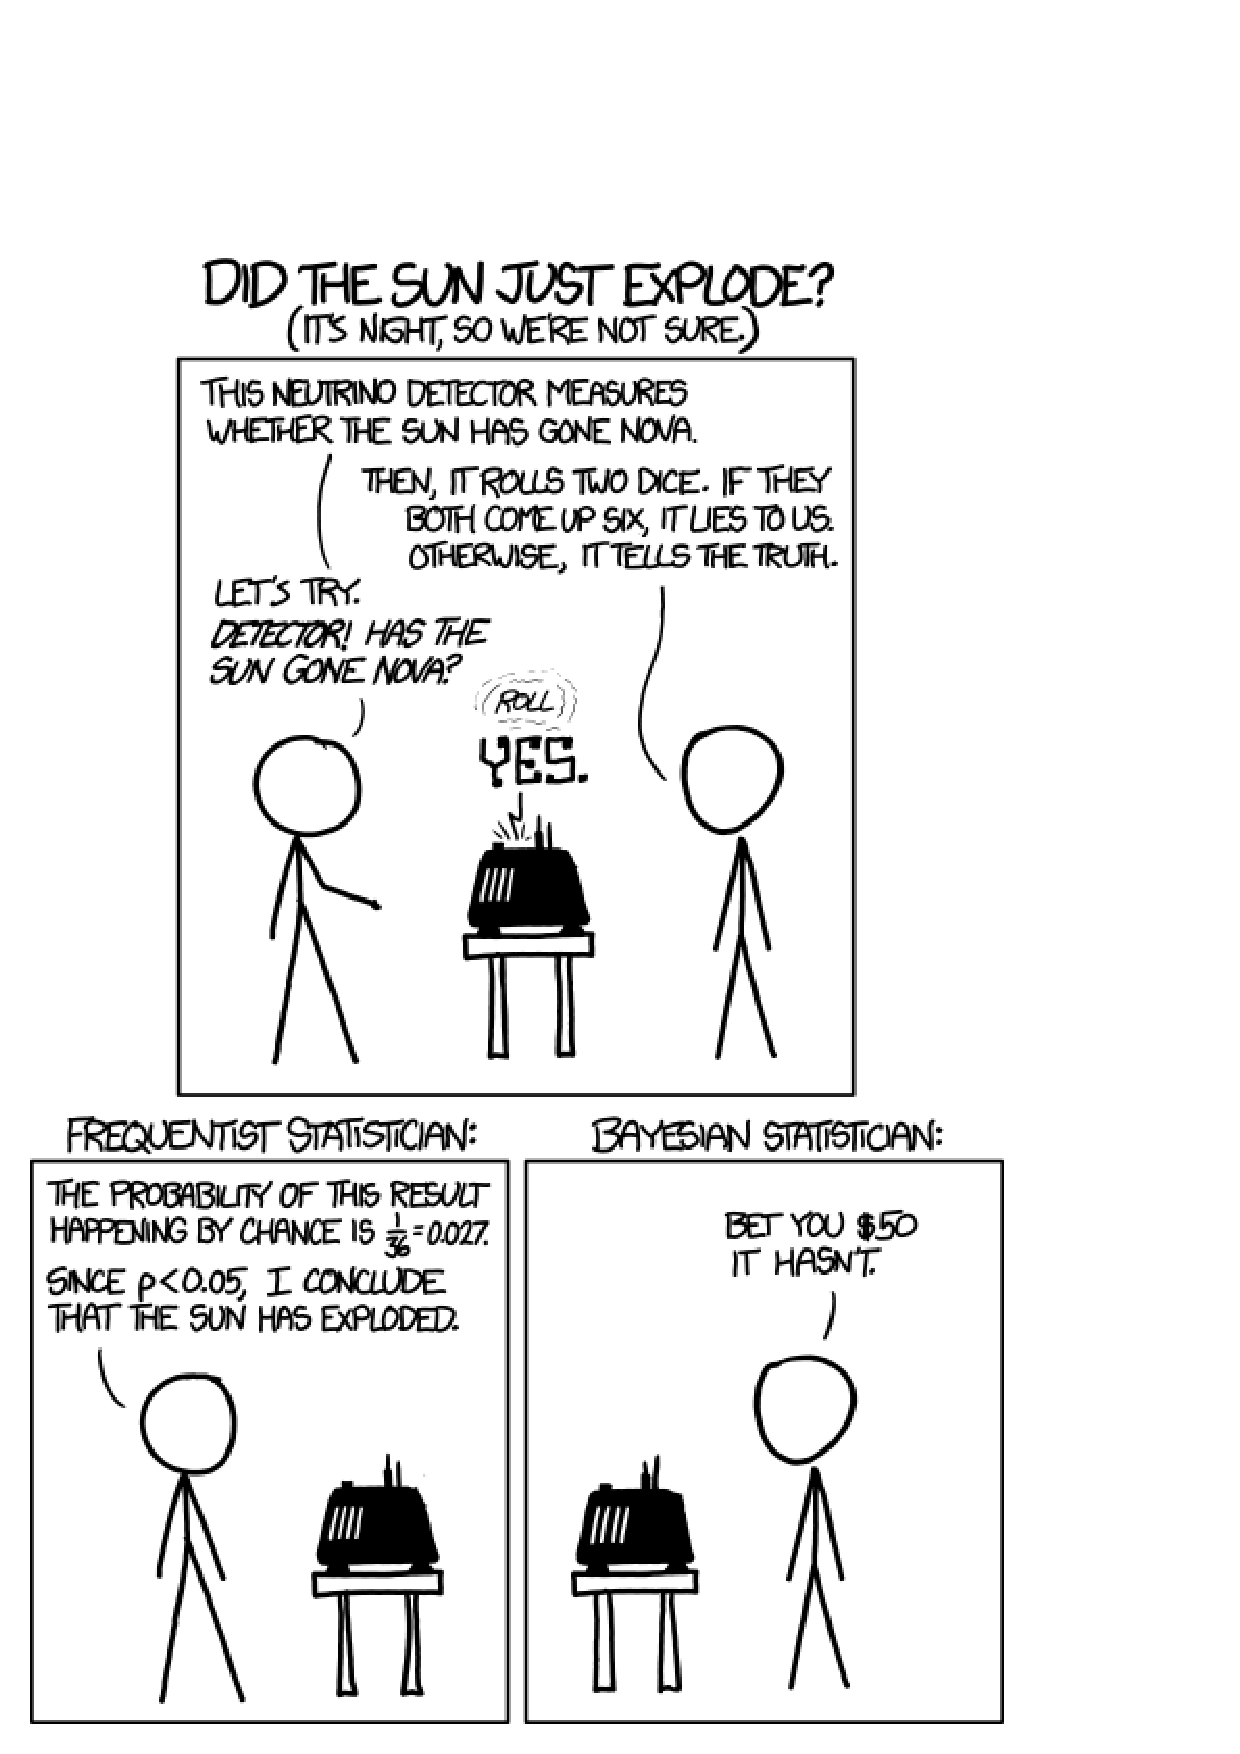
\includegraphics[width=8cm]{frequentists_vs_bayesians.png}
        \else
            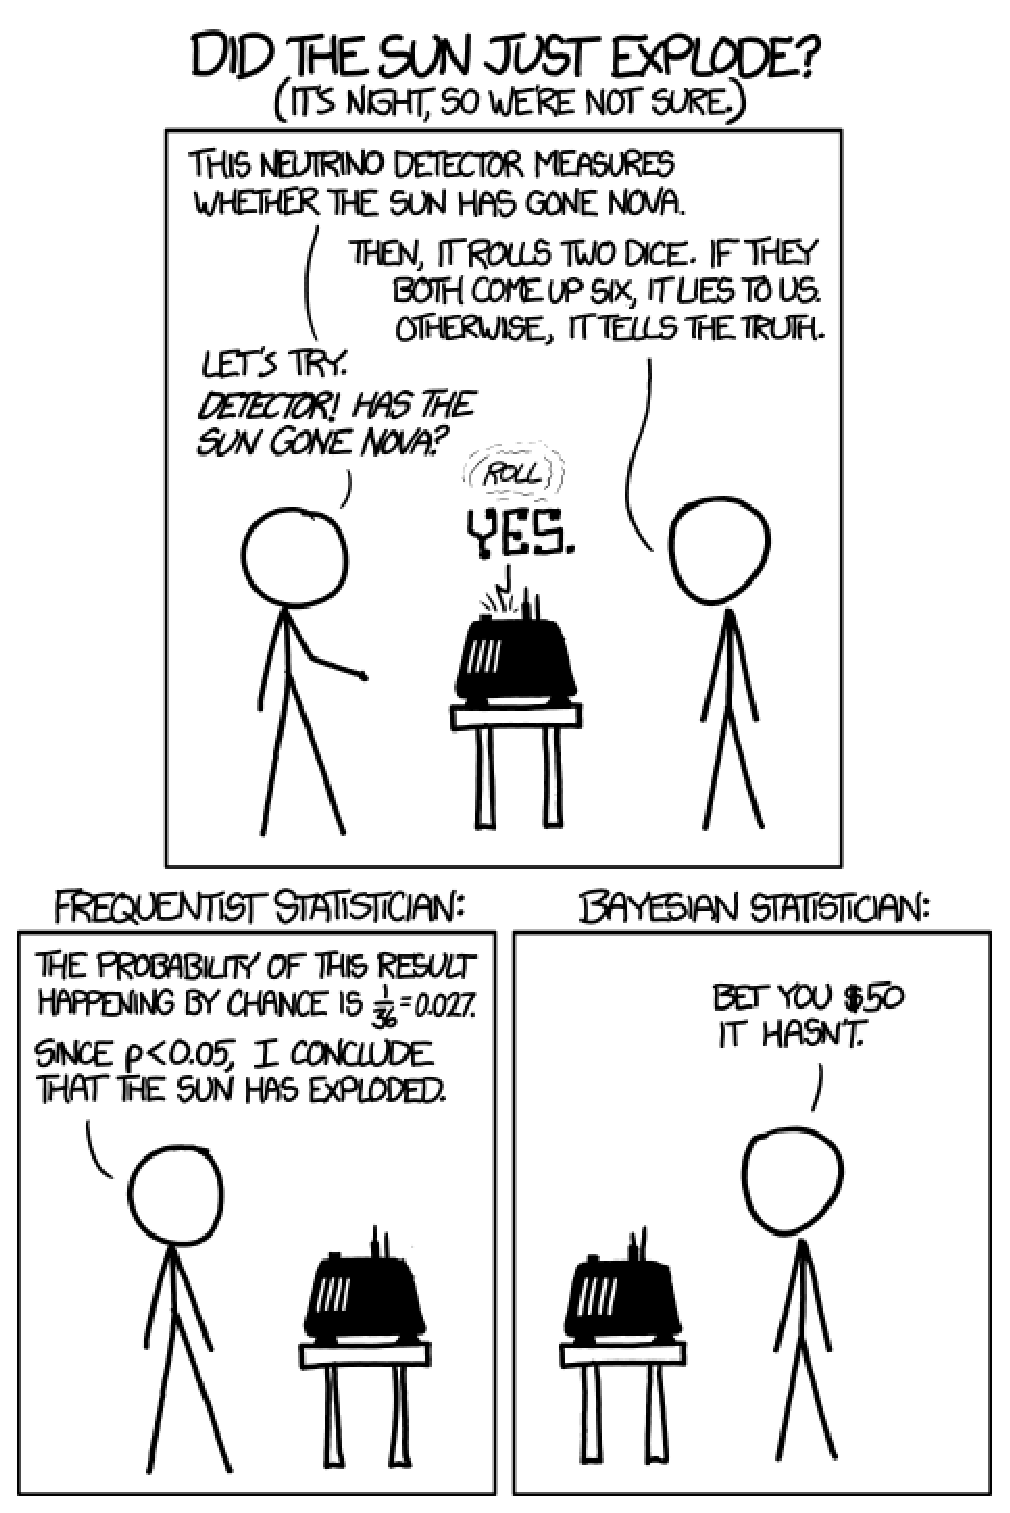
\includegraphics[width=8cm]{frequentists_vs_bayesians.eps}

            \fi

            \url{http://xkcd.com/1132/}, image publiée sous licence \href{http://xkcd.com/license.html}{CreativeCommons}.

\end{center}


%&=& &=& &=& &=& &=& &=& &=& &=& &=& &=& &=& &=& &=& &=& &=& &=& &=& &=& &=& &=& &=& &=& &=& 
\part{Trucs pour les AP}
%&=& &=& &=& &=& &=& &=& &=& &=& &=& &=& &=& &=& &=& &=& &=& &=& &=& &=& &=& &=& &=& &=& &=& 
% This is part of Un soupçon de mathématique sans être agressif pour autant
% Copyright (c) 2014
%   Laurent Claessens
% See the file fdl-1.3.txt for copying conditions.

%+++++++++++++++++++++++++++++++++++++++++++++++++++++++++++++++++++++++++++++++++++++++++++++++++++++++++++++++++++++++++++ 
\section{Origami}
%+++++++++++++++++++++++++++++++++++++++++++++++++++++++++++++++++++++++++++++++++++++++++++++++++++++++++++++++++++++++++++

La feuille distribuée pour la découverte du théorème d'Haga.

% THÉORÈME DE HAGA POUR L'AP
\begin{feuilleExo}{Théorème de Haga}

%\begin{wrapfigure}{r}{10.cm}
    \begin{center}
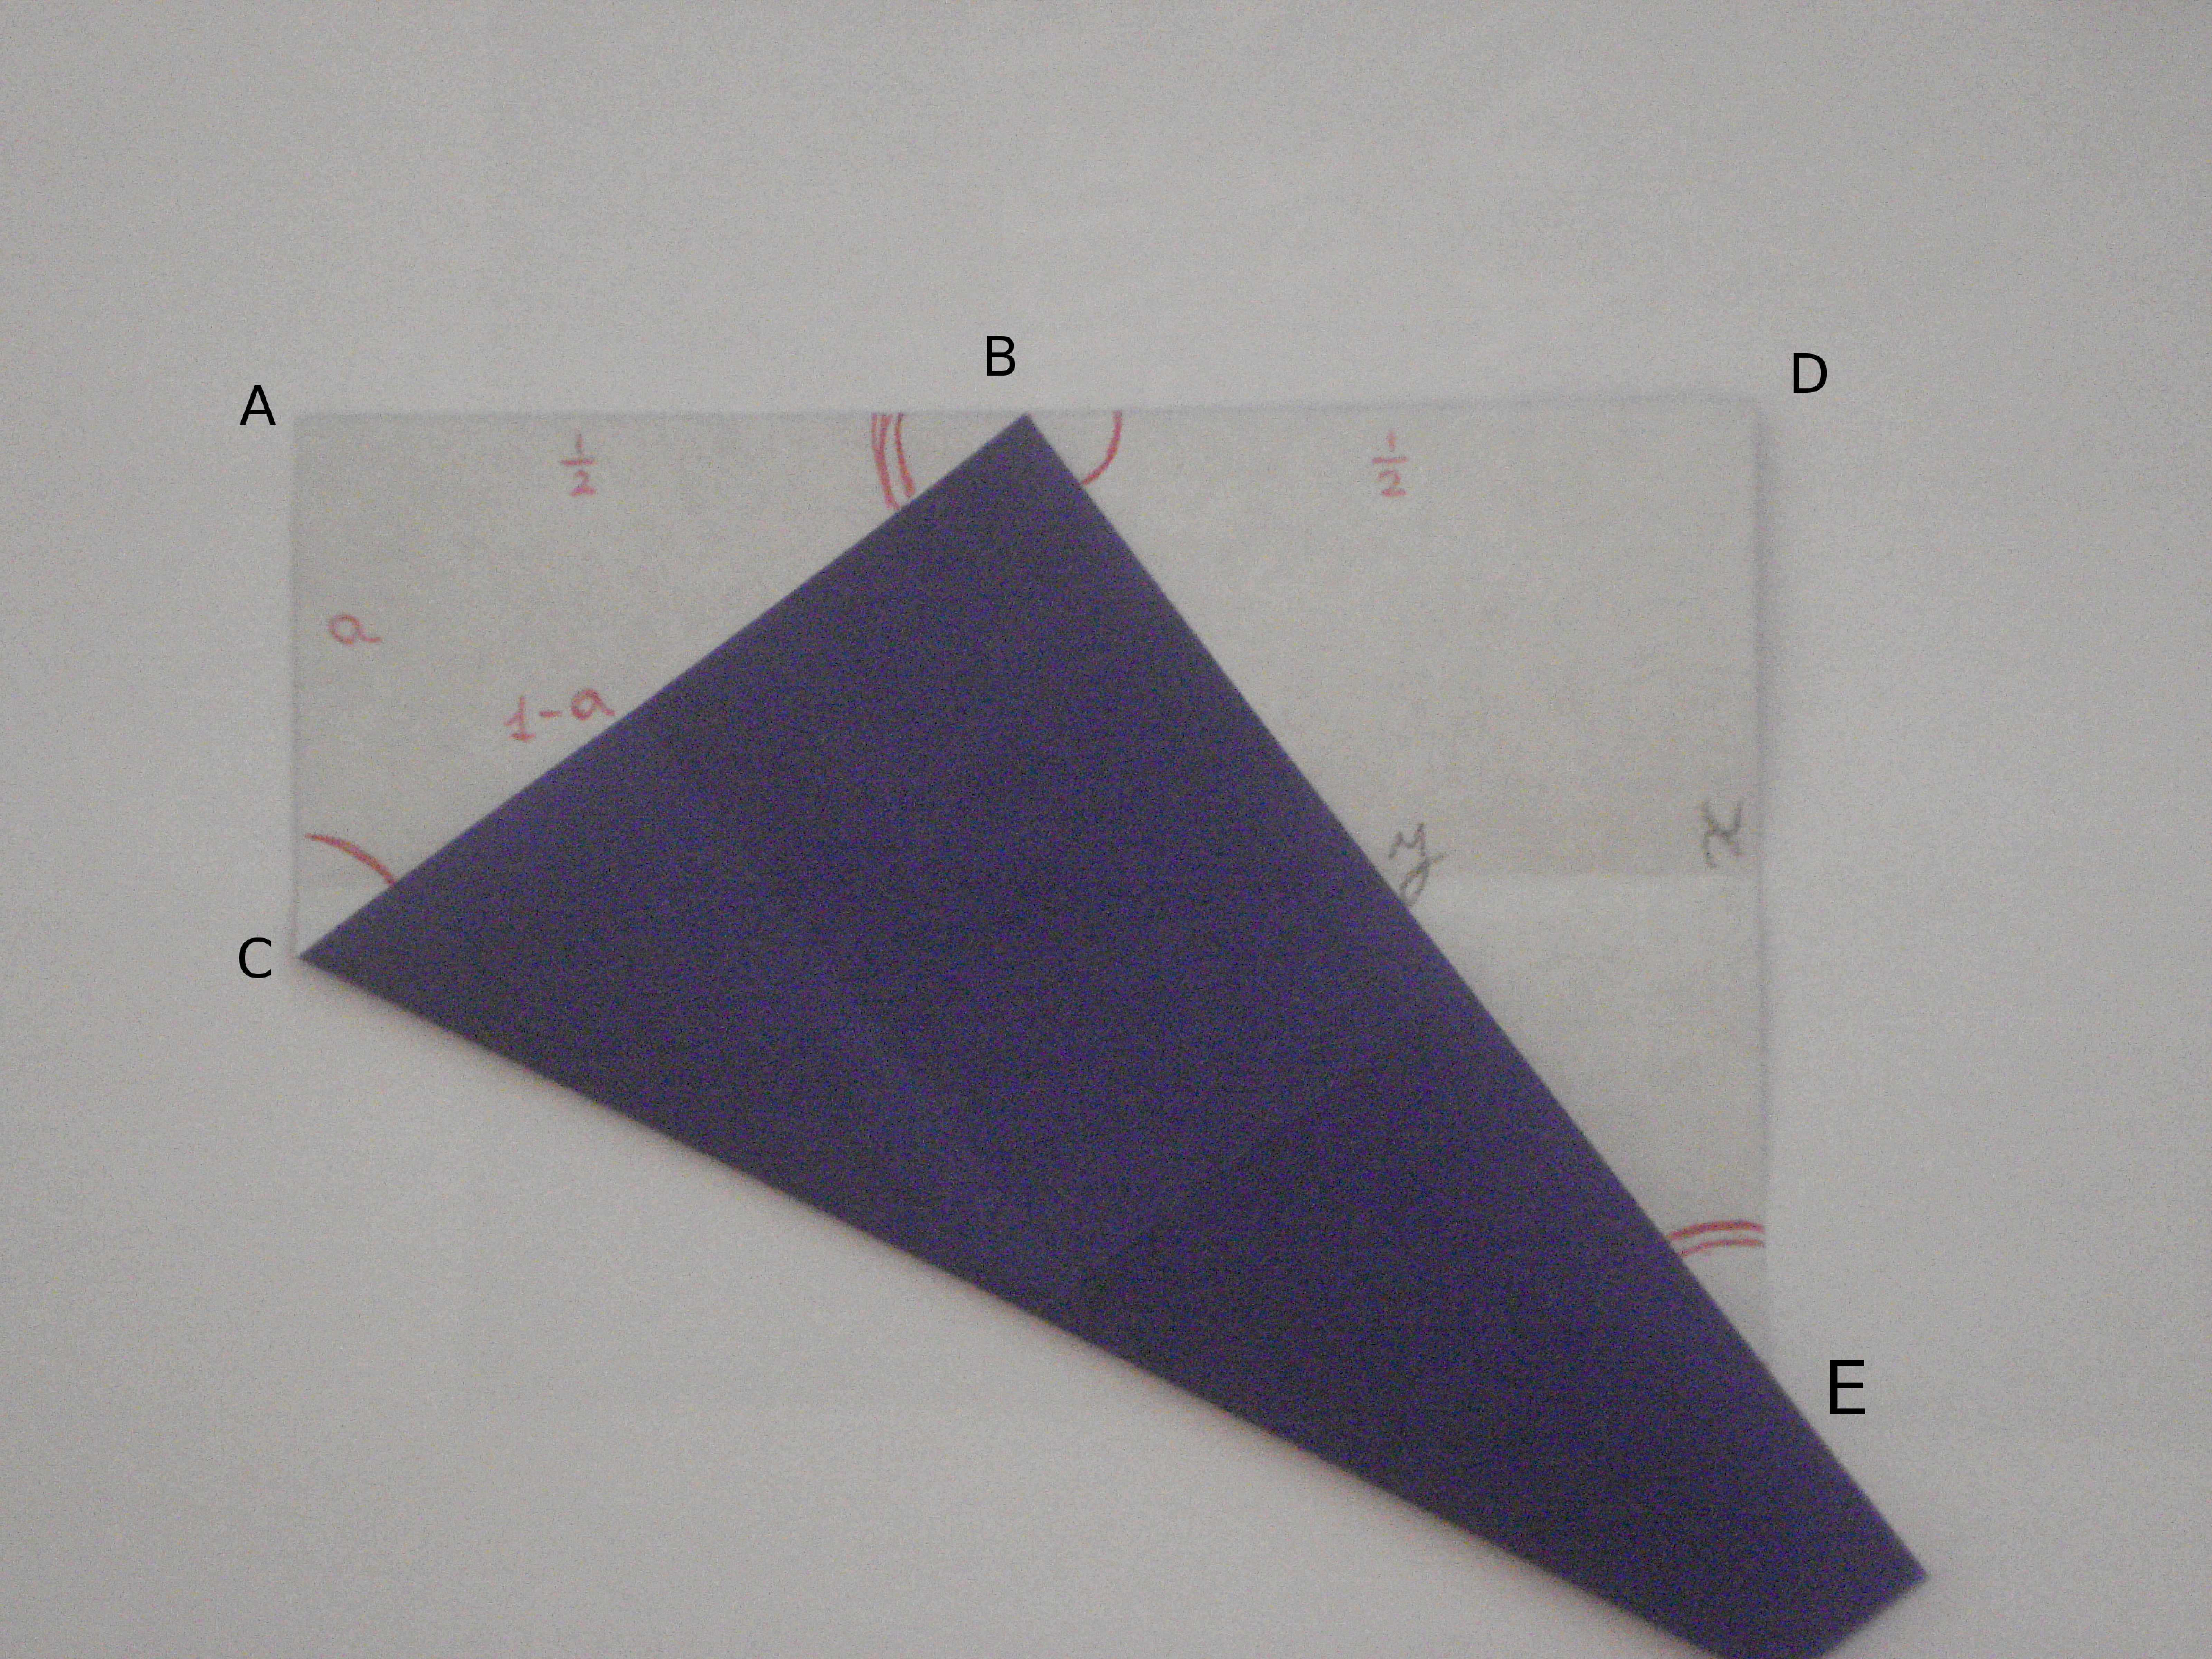
\includegraphics[width=10cm]{Haga.pdf}
    \end{center}
%\end{wrapfigure}

\paragraph{Un peu de Pythagore}


Nous avons appelé \( a\) la longueur du segment \( [AC]\). Pourquoi \( BC=1-a\) ? Quelle est la valeur de \( a\) ?

\paragraph{Question d'angle}

Notons \( \hat B_1\) et \( \hat B_2\) les deux angles situés au point \( B\) (\( \hat B_1\) est celui du triangle \( ABC\)).
\begin{enumerate}
    \item
        Combien vaut \( \hat B_1+\hat B_2\) ?
    \item
        Combien vaut \( \hat B_1+\hat C\) ?
    \item
        En déduire que \( \hat B_2=\hat C\).
\end{enumerate}
Pourquoi \( \hat B_1=\hat E\) ?

\paragraph{Triangles semblables}

Les triangles \( ABC\) et \( BDE\) sont donc deux triangles ayant les mêmes angles; ils sont donc semblables et donc «proportionnels». De la même façon que pour Thalès, nous pouvons écrire les égalités «grand divisé par petit» :
\begin{equation}
    \frac{ DE }{ BD }=\frac{ AB }{ AC }.
\end{equation}
Reporter les valeurs connues et déduire la valeur de \( x=DE\).

\paragraph{Conclusion}

Sachant la valeur de \( x\), conclure que nous avons bien obtenu un pliage coupant en trois le côté du carré.

\end{feuilleExo}


Les diapositives projetées pour la présentation. 

\newpage
\subsection{Théorème de Haga (Pythagore)}

    \begin{multicols}{2}

    \begin{center}        
        \includegraphics[width=5cm]{haga_coupe_anote}
    \end{center}


    Pythagore dans le triangle \( ABC\) : \( a^2+\left( \frac{ 1 }{2} \right)^2=(1-a)^2\).

    \( \Rightarrow \, a=\frac{ 3 }{ 8 }\).
    \end{multicols}

    
\newpage
\subsection{Théorème de Haga (angles)}
    \begin{multicols}{2}

    \begin{center}        
        \includegraphics[width=5cm]{haga_coupe_anote}
    \end{center}

    \begin{subequations}
        \begin{numcases}{}
            \hat B_1+\hat B_2=90\\
            \hat B_1+\hat C=90\\
            \hat B_2+\hat E=90
        \end{numcases}
    \end{subequations}

    \( \Rightarrow \,   \hat B_2=\hat C \) et \( \hat B_1=\hat E\).
    \end{multicols}


    \begin{center}
        Les triangles \( ABC\) et \( BDE\) sont semblables.
    \end{center}

\newpage
\subsection{Théorème de Haga (proportionnalité)}
    \begin{multicols}{2}

    \begin{center}        
        \includegraphics[width=5cm]{haga_coupe_anote}
    \end{center}

    \begin{equation}
        \frac{ DE }{ AB }=\frac{ BD }{ AC }
    \end{equation}
    \begin{equation}
        \frac{ DE }{ \frac{ 1 }{2} }=\frac{ \frac{ 1 }{2} }{ \frac{ 3 }{ 8 } }
    \end{equation}
    \begin{equation}
        2DE=\frac{ 4 }{ 3 }
    \end{equation}
    \begin{equation}
        DE=\frac{2}{ 3 }.
    \end{equation}
    \end{multicols}


%&=& &=& &=& &=& &=& &=& &=& &=& &=& &=& &=& &=& &=& &=& &=& &=& &=& &=& &=& &=& &=& &=& &=& 
\part{Python}
%&=& &=& &=& &=& &=& &=& &=& &=& &=& &=& &=& &=& &=& &=& &=& &=& &=& &=& &=& &=& &=& &=& &=& 
% This is part of Un soupçon de mathématique sans être agressif pour autant
% Copyright (c) 2012
%   Laurent Claessens
% See the file fdl-1.3.txt for copying conditions.

\chapter{Structures de base}

\begin{remark}
    Certains bouts de codes donnés ici commencent par la ligne
    \begin{quote}
        \info{\# -*- coding: utf8 -*-}
    \end{quote}
    Si vous savez ce que signifie «\wikipedia{fr}{Utf8}{utf8}», vous devriez deviner à quoi sert cette ligne. Sinon c'est pas grave : vous n'êtes pas \emph{obligés} de l'écrire dans vos programmes, mais c'est une bonne habitude à prendre. Nous en reparlerons peut-être plus tard.
\end{remark}

%---------------------------------------------------------------------------------------------------------------------------
\subsection{La fonction \info{print}}
%---------------------------------------------------------------------------------------------------------------------------

Python ne prend pas d'initiatives. Si vous ne lui demandez pas d'écrire quelque chose, il n'écrira rien. La commande la plus courante\footnote{Bien entendu, python permet de programmer des fenêtres, des boutons et autres boites de dialogue, auquel cas ce ne sera plus la commande \info{print} qui jouera.} pour afficher quelque chose à l'écran est la commande \info{print}. 
\begin{enumerate}
    \item
        Pour afficher la valeur d'une variable \info{a}, mettre \info{print(a)}.
    \item
        Pour afficher un texte (par exemple «bonjour» ), mettre des guillemets : \info{print(``bonjour'')}.
\end{enumerate}
Si vous voulez afficher plusieurs choses, vous les séparez par une virgule.

\lstinputlisting{ex_print.py}

donne

\lstinputlisting[title=Résultat]{res_ex_print.txt}

Notez que les lignes qui commencent par \# ne sont pas prises en compte. Cela permet au programmeur de mettre des notes pour lui-même. N'hésitez pas à en mettre pour rendre votre code plus lisible.

\Exo{Premiere-0037}

%+++++++++++++++++++++++++++++++++++++++++++++++++++++++++++++++++++++++++++++++++++++++++++++++++++++++++++++++++++++++++++
\section{Listes}
%+++++++++++++++++++++++++++++++++++++++++++++++++++++++++++++++++++++++++++++++++++++++++++++++++++++++++++++++++++++++++++

Une liste est une collection ordonnée d'éléments. Elle se définit avec des crochets.

\lstinputlisting{ex_listes.py}

donne

\lstinputlisting[title=Résultat]{res_ex_listes.txt}

Nous pouvons ajouter un élément à une liste en utilisant la \emph{méthode} \info{append}, et retrouver un élément d'une liste par son numéro (attention : python numérote à partie de zéro), en demandant par exemple \info{A[4]} pour l'élément numéro \( 4\) de la liste \info{A}. Cela sera donc le cinquième élément de la liste. Cas spécial : le dernier élément de la liste est le numéro \( -1\).

\lstinputlisting{ex_listes2.py}

donne

\lstinputlisting[title=Résultat]{res_ex_listes2.txt}


\Exo{Premiere-0033}


La multiplication d'une liste par un nombre donne la liste contenant plusieurs fois la liste originale. Nous ajoutons une liste à une autre en utilisant la méthode \info{extend}.


\lstinputlisting{ex_listes3.py}

donne

\lstinputlisting[title=Résultat]{res_ex_listes3.txt}


\Exo{Premiere-0034}

%+++++++++++++++++++++++++++++++++++++++++++++++++++++++++++++++++++++++++++++++++++++++++++++++++++++++++++++++++++++++++++
\section{Quelque mots à propos des fonctions}
%+++++++++++++++++++++++++++++++++++++++++++++++++++++++++++++++++++++++++++++++++++++++++++++++++++++++++++++++++++++++++++

%---------------------------------------------------------------------------------------------------------------------------
\subsection{Choses Basiques}
%---------------------------------------------------------------------------------------------------------------------------

Si un calcul doit être refait plusieurs fois dans un même programme, il est bon d'écrire une fonction qui sera appelée à chaque fois. En python, une fonction se déclare avec le mot-clef \info{def} comme ceci :
\begin{quote}
    \info{def\ nom\_de\_ma\_fonction(a,b):}
\end{quote}
où \info{a} et \info{b} seront les arguments de la fonction. Il peut y en avoir un seul, deux, ou plus (pas de limites), ou pas du tout. Une fonction peut afficher et calculer autant de résultats intermédiaires que l'on veut. 

\lstinputlisting{ex_fonction.py}

donne

\lstinputlisting[title=Résultat]{res_ex_fonction.txt}

Cette fonction ne fait qu'afficher du texte, mais ne retourne pas de valeurs. Voici une fonction qui retourne \( 1\) si le nombre donné est plus grand ou égal à zéro et retourne \( -1\) si il est négatif.


\lstinputlisting{ex_fonction2.py}

donne

\lstinputlisting[title=Résultat]{res_ex_fonction2.txt}

%---------------------------------------------------------------------------------------------------------------------------
\subsection{Pour aller plus loin}
%---------------------------------------------------------------------------------------------------------------------------

La fonction de l'exemple précédent peut être simplifiée en sachant que dès que une instruction \info{return} est rencontrée, l'exécution de la fonction est \emph{immédiatement} stoppée et la valeur est retournée. Nous pouvons donc écrire

\lstinputlisting{ex_fonction3.py}

Si le nombre donné est positif, un \info{return} est rencontré à l'intérieur du \info{if}, et l'autre \info{return} n'est jamais rencontré.

D'autre part, une fonction peut vraiment prendre \emph{n'importe quoi} comme argument, y compris des autres fonctions. Dans l'exemple suivant, la fonction \info{evaluation} prend un argument une fonction et un nombre, et retourne la fonction évaluée en ce nombre.

\lstinputlisting{ex_fonction4.py}

donne

\lstinputlisting[title=Résultat]{res_ex_fonction4.txt}


%+++++++++++++++++++++++++++++++++++++++++++++++++++++++++++++++++++++++++++++++++++++++++++++++++++++++++++++++++++++++++++
\section{Moyenne, médiane, quartiles}
%+++++++++++++++++++++++++++++++++++++++++++++++++++++++++++++++++++++++++++++++++++++++++++++++++++++++++++++++++++++++++++
\label{SecZYftar}

%---------------------------------------------------------------------------------------------------------------------------
\subsection{Moyenne}
%---------------------------------------------------------------------------------------------------------------------------

\begin{example}     \label{ExerfDMnv}
    % Note : la liste ci-dessous est codée en dur dans les scripts d'exemples. Si on la modifie, il faut modifier les scripts.
    Un magasin de chaussures a vendu des tailles entre \( 40\) et \( 45\) suivant la distribution suivante :
    \begin{center}
        \begin{tabular}{|l||c|c|c|c|c|c|}
            \hline
            taille \( x_i\)&40&41&42&43&44&45\\
            \hline
            effectifs \( n_i\)&3&5&10&8&2&4\\
            \hline
        \end{tabular}
    \end{center}
    Nous voudrions calculer la moyenne, la médiane et les quartiles de la distribution des tailles de chaussures. Nous allons nous occuper de cela dans les pages qui viennent.
\end{example}
    
    Pour calculer la moyenne d'une liste, nous devons savoir la longueur et la somme de ses éléments. Python fournit cela assez rapidement. Si \info{A} est une liste,
    \begin{enumerate}
        \item
            \info{len(A)} est la longueur de \info{A},
        \item
            \info{sum(A)} est la somme de ses éléments.
    \end{enumerate}
    
\Exo{Premiere-0035}
    
Le programme suivant écrit la moyenne de la liste des tailles de chaussures de l'exemple \ref{exnXIMeL}.

\lstinputlisting{chaussures.py}

%\lstinputlisting{res_chaussures.txt}

%---------------------------------------------------------------------------------------------------------------------------
\subsection{Premier et troisième quartiles}
%---------------------------------------------------------------------------------------------------------------------------

Pour les quartiles, nous nous rappelons que si \( n\) est le nombre de valeurs, alors le rang du premier quartile est le premier entier supérieur à \( n/4\); et le rang du troisième quartile est le premier entier supérieur à \( 3n/4\). Par exemple si il y a \( 15\) données, nous calculons \( 3\times 15/3= 11.25\), et le troisième quartile sera la douzième valeur.


Bien entendu python possède une commande qui retourne le premier entier supérieur à un nombre donné. C'est la commande \info{ceil} du module \info{math}. En pratique :

\lstinputlisting{exemple_ceil.py}

donne 

\lstinputlisting{res_exemple_ceil.txt}
De même la fonction \info{math.floor} retourne le premier entier inférieur à un nombre donné. Par exemple \info{math.floor(3.89)} vaut \( 3\).

La ligne \info{import math} s'appelle «importer le module math», et nous n'en dirons sans doute pas plus sur la notion d'import de module. Le module \info{math} contient encore de nombreuses fonctions mathématiques qui transforment python en une très puissante\footnote{Pour donner une idée, la mémoire disponible sur des calculatrices modernes est à peu près la même que celle qui était disponible sur Apple II au début des années 1980; avec python vous pouvez exploiter toute la mémoire de votre ordinateur, ou de votre téléphone ou de votre tablette ou de quoi que ce soit sur lequel vous avez python.} calculatrice scientifique.


\Exo{Premiere-0036}

\lstinputlisting{premier_quartile.py}

Et voici pour la médiane :

\lstinputlisting{mediane.py}


\Exo{Premiere-0038}

%+++++++++++++++++++++++++++++++++++++++++++++++++++++++++++++++++++++++++++++++++++++++++++++++++++++++++++++++++++++++++++
\section{Suite définie par récurrence} 
%+++++++++++++++++++++++++++++++++++++++++++++++++++++++++++++++++++++++++++++++++++++++++++++++++++++++++++++++++++++++++++

Soit une suite définie par récurrence

\begin{subequations}
    \begin{numcases}{}
    u_0=10\\
    u_{n+1}=2u_n.
    \end{numcases}
\end{subequations}

Nous voudrions pouvoir répondre à deux types de questions :
\begin{enumerate}
    \item
        construire une liste contenant les \( 100\) premiers termes de la suite;
    \item
        savoir quel est le premier terme à dépasser un million.
\end{enumerate}

Avant de se lancer, nous devons nous poser une question de vocabulaire : est-ce que le centième terme de la suite \( u\) est \( u_{100}\) ou \( u_{99}\) ? Le premier terme étant \( u_0\), le centième est bien \( u_{99}\).

\lstinputlisting{recurrence1.py}

donne

\lstinputlisting{res_recurrence1.txt}

Notons que la ligne \info{print(u[100])} plante avec l'erreur \info{list index out of range}, c'est à dire que la liste \info{u} n'a pas d'élément \info{u[100]}, ce qui est normal parce qu'elle contient \( 100\) éléments et que la numérotation commence à zéro.


\Exo{Premiere-0039}


En ce qui concerne la possibilité de trouver le premier élément qui dépasse le million, le programme suivant donne deux méthodes.

\lstinputlisting{recurrence2.py}

donne

\lstinputlisting{res_recurrence2.txt}

Notons que la première méthode donne \( 17\) et la seconde donne \( 18\). Qui a raison ? Le \( 18\) de la seconde méthode est la longueur de la liste construite, donc il indique que le premier terme à passer le million est \( u_{17}\) (vu que le premier terme est \( u_0\), la longueur est toujours un plus grande que le numéro du dernier élément).

La réponse est donc que \( u_{17}\) est le premier élément à être plus grand que un million, mais \( u_{17}\) est le dix-huitième élément de la liste.


%+++++++++++++++++++++++++++++++++++++++++++++++++++++++++++++++++++++++++++++++++++++++++++++++++++++++++++++++++++++++++++
\section{Exercices}
%+++++++++++++++++++++++++++++++++++++++++++++++++++++++++++++++++++++++++++++++++++++++++++++++++++++++++++++++++++++++++++


\Exo{Premiere-0027}




\part{Exercices}


\chapter{Autres exercices}
%---------------------------------------------------------------------------------------------------------------------------
\subsection{Égalité de fonctions}
%---------------------------------------------------------------------------------------------------------------------------

Les identités remarquables :
\begin{subequations}
    \begin{align}
        (a+b)^2=a^2+2ab+b^2\\
        (a-b)^2=a^2-2ab+b^2\\
        (a+b)(a-b)=a^2-b^2.
    \end{align}
\end{subequations}

\Exo{smath-0042}
\Exo{smath-0043}
\Exo{smath-0044}
\Exo{smath-0045}
\Exo{smath-0046}

%+++++++++++++++++++++++++++++++++++++++++++++++++++++++++++++++++++++++++++++++++++++++++++++++++++++++++++++++++++++++++++ 
\section{Proportions, pourcentage}
%+++++++++++++++++++++++++++++++++++++++++++++++++++++++++++++++++++++++++++++++++++++++++++++++++++++++++++++++++++++++++++

\Exo{Seconde-0023}
\Exo{smath-0296}
\Exo{Seconde-0031}
\Exo{Seconde-0025}


%+++++++++++++++++++++++++++++++++++++++++++++++++++++++++++++++++++++++++++++++++++++++++++++++++++++++++++++++++++++++++++ 
\section{À l'ordinateur}
%+++++++++++++++++++++++++++++++++++++++++++++++++++++++++++++++++++++++++++++++++++++++++++++++++++++++++++++++++++++++++++

\lstinputlisting{IF_TD_seconde.py}
\Exo{smath-0338}
\Exo{smath-0385}
\Exo{smath-0604}

%---------------------------------------------------------------------------------------------------------------------------
\subsection{Théorie}
%---------------------------------------------------------------------------------------------------------------------------

\Exo{smath-0056}
\Exo{smath-0057}
\Exo{smath-0058}




%\input{de_svt}

\part{Autres}
Cette partie contient des choses vues au lycée mais pas spécialement dans mes classes. Ce sont surtout des choses pompées de première année SVT à l'université de Franche-Comté.

\input{theorie}
\input{rappelsLog}


\section{Exponentielles et logarithmes}
% This is part of Exercices de mathématique pour SVT
% Copyright (c) 2010-2011
%   Laurent Claessens et Carlotta Donadello
% See the file fdl-1.3.txt for copying conditions.




\section{Fonctions et graphes}
\input{TD1.tex}


\section{Limites du côté de l'infini}
\Exo{SVT-0001}
\Exo{TD3-0003}

\section{Limite de suites}
\input{TD3.tex}

\section{Étude de fonctions, première partie}
\Exo{TD2-1}
\Exo{TD2A-2}
\Exo{TD2B_1}       
\Exo{TD2-2}

\section{Étude de fonctions, suite}
\Exo{TD4-0001}
\Exo{TD4-0002}
\Exo{TD4-0003}
\Exo{TD4-0004}
\Exo{TD4-0005}

\section{Intégration}
\input{TD5.tex}

\section{Équations différentielles}
\input{TD6A.tex}

\section{Révisions}
\input{TD_revisions.tex}



\Exo{interro-0002}
\Exo{interro-0003}
\Exo{interro-0004}
\Exo{interro-0005}
\Exo{interro-0007}
\Exo{interro-0008}


\Exo{DS2010-1-0001}
\Exo{DS2010-1-0002}
\Exo{DS2010-1-0003}
\Exo{DS2010-1-0004}
\Exo{DS2010-1-0005}

\Exo{DS2010bis-0001}
\Exo{DS2010bis-0002}
\Exo{DS2010bis-0003}
\Exo{DS2010bis-0004}
\Exo{DS2010bis-0005}


\Exo{ExamenDecembre2010-0001}
\Exo{ECdecembre2010-0001}
\Exo{ECdecembre2010-0002}
\Exo{ECdecembre2010-0003}
\Exo{ECdecembre2010-0004}
\Exo{ExamenDecembre2010-0002}
\Exo{ExamenDecembre2010-0003}
\Exo{ExamenDecembre2010-0004}
\Exo{ExamenDecembre2010-0005}
\Exo{Exosenvrac-0001} 
\Exo{Exosenvrac-0015}
\Exo{Exosenvrac-0015A}
\Exo{Exosenvrac-0006}
\Exo{Exosenvrac-0009}


\corrChapitre{Corrections de certains exercices}

\input{fdl-1.3.tex}

\bibliographystyle{unsrt}           % unsrt fait que la biblio arrive dans l'ordre de citation au lieu de l'ordre alphabétique.
\bibliography{mazhe}

\printindex

\end{document}

\Exo{smath-0711}
\Exo{smath-0712}
\Exo{smath-0713}
\Exo{smath-0714}
\Exo{smath-0715}
\Exo{smath-0716}
\Exo{smath-0717}
\Exo{smath-0718}
\Exo{smath-0719}
\Exo{smath-0720}
\Exo{smath-0721}
\Exo{smath-0722}
\Exo{smath-0723}
\Exo{smath-0724}
\Exo{smath-0725}
\Exo{smath-0726}
\Exo{smath-0727}
\Exo{smath-0728}
\Exo{smath-0729}
\Exo{smath-0730}
\Exo{smath-0731}
\Exo{smath-0732}
\Exo{smath-0733}
\Exo{smath-0734}
\Exo{smath-0735}
\Exo{smath-0736}
\Exo{smath-0737}
\Exo{smath-0738}
\Exo{smath-0739}
\Exo{smath-0740}
\Exo{smath-0741}
\Exo{smath-0742}
\Exo{smath-0743}
\Exo{smath-0744}
\Exo{smath-0745}
\Exo{smath-0746}
\Exo{smath-0747}
\Exo{smath-0748}
\Exo{smath-0749}
\Exo{smath-0750}
\Exo{smath-0751}
\Exo{smath-0752}
\Exo{smath-0753}
\Exo{smath-0754}
\Exo{smath-0755}
\Exo{smath-0756}
\Exo{smath-0757}
\Exo{smath-0758}
\Exo{smath-0759}
\Exo{smath-0760}
\Exo{smath-0761}
\Exo{smath-0762}
\Exo{smath-0763}
\Exo{smath-0764}
\Exo{smath-0765}
\Exo{smath-0766}
\Exo{smath-0767}
\Exo{smath-0768}
\Exo{smath-0769}
\Exo{smath-0770}
\Exo{smath-0771}
\Exo{smath-0772}
\Exo{smath-0773}
\Exo{smath-0774}
\Exo{smath-0775}
\Exo{smath-0776}
\Exo{smath-0777}
\Exo{smath-0778}
\Exo{smath-0779}
\Exo{smath-0780}
\Exo{smath-0781}
\Exo{smath-0782}
\Exo{smath-0783}
\Exo{smath-0784}
\Exo{smath-0785}
\Exo{smath-0786}
\Exo{smath-0787}
\Exo{smath-0788}
\Exo{smath-0789}
\Exo{smath-0790}
\Exo{smath-0791}
\Exo{smath-0792}
\Exo{smath-0793}
\Exo{smath-0794}
\Exo{smath-0795}
\Exo{smath-0796}
\Exo{smath-0797}
\Exo{smath-0798}
\Exo{smath-0799}
\Exo{smath-0800}

\lstinputlisting{ex_algo25.py}
\lstinputlisting{ex_algo26.py}
\lstinputlisting{ex_algo27.py}
\lstinputlisting{ex_algo28.py}
\lstinputlisting{ex_algo29.py}
\lstinputlisting{ex_algo30.py}
\lstinputlisting{ex_algo31.py}
\lstinputlisting{ex_algo32.py}
\lstinputlisting{ex_algo33.py}
\lstinputlisting{ex_algo34.py}
\lstinputlisting{ex_algo35.py}
\lstinputlisting{ex_algo36.py}
\lstinputlisting{ex_algo37.py}
\lstinputlisting{ex_algo38.py}
\lstinputlisting{ex_algo39.py}
\lstinputlisting{ex_algo40.py}
\lstinputlisting{ex_algo41.py}
\lstinputlisting{ex_algo42.py}
\lstinputlisting{ex_algo43.py}
\lstinputlisting{ex_algo44.py}
\lstinputlisting{ex_algo45.py}
\lstinputlisting{ex_algo46.py}
\lstinputlisting{ex_algo47.py}
\lstinputlisting{ex_algo48.py}
\lstinputlisting{ex_algo49.py}
\lstinputlisting{ex_algo50.py}
\lstinputlisting{ex_algo51.py}
\lstinputlisting{ex_algo52.py}
\lstinputlisting{ex_algo53.py}
\lstinputlisting{ex_algo54.py}
\lstinputlisting{ex_algo55.py}
\lstinputlisting{ex_algo56.py}
\lstinputlisting{ex_algo57.py}
\lstinputlisting{ex_algo58.py}
\lstinputlisting{ex_algo59.py}
\lstinputlisting{ex_algo60.py}
\lstinputlisting{ex_algo61.py}
\lstinputlisting{ex_algo62.py}
\lstinputlisting{ex_algo63.py}
\lstinputlisting{ex_algo64.py}
\lstinputlisting{ex_algo65.py}
\lstinputlisting{ex_algo66.py}
\lstinputlisting{ex_algo67.py}
\lstinputlisting{ex_algo68.py}
\lstinputlisting{ex_algo69.py}
\lstinputlisting{ex_algo70.py}
\lstinputlisting{ex_algo71.py}
\lstinputlisting{ex_algo72.py}
\lstinputlisting{ex_algo73.py}
\lstinputlisting{ex_algo74.py}
\lstinputlisting{ex_algo75.py}
\lstinputlisting{ex_algo76.py}
\lstinputlisting{ex_algo77.py}
\lstinputlisting{ex_algo78.py}
\lstinputlisting{ex_algo79.py}
\lstinputlisting{ex_algo80.py}
\lstinputlisting{ex_algo81.py}
\lstinputlisting{ex_algo82.py}
\lstinputlisting{ex_algo83.py}
\lstinputlisting{ex_algo84.py}
\lstinputlisting{ex_algo85.py}
\lstinputlisting{ex_algo86.py}
\lstinputlisting{ex_algo87.py}
\lstinputlisting{ex_algo88.py}
\lstinputlisting{ex_algo89.py}
\lstinputlisting{ex_algo90.py}
\lstinputlisting{ex_algo91.py}
\lstinputlisting{ex_algo92.py}
\lstinputlisting{ex_algo93.py}
\lstinputlisting{ex_algo94.py}
\lstinputlisting{ex_algo95.py}
\lstinputlisting{ex_algo96.py}
\lstinputlisting{ex_algo97.py}
\lstinputlisting{ex_algo98.py}

%TODO : en classe de seconde, il faudrait toujours parler de f(x)=mx+p au lieu de ax+b.
